% Full thesis: Chapters 1--6, Appendices, Bibliography.
% Front matter: TOC, LOF, LOT, List of Acronyms, Abstract (each on own page). Abstract last. Chapter 1 starts page 1 (odd).

\documentclass{thesis-report}

\title{Deploying an Autonomous Indoor Robot with Laser Mapping and Multi-Hop Networking for Disaster Site Exploration}
\author{Habeel Ali}
\date{\today}

\begin{document}

% No \maketitle here; add cover pages before this file or in a separate front matter file.

% --- Front matter: no page numbers on TOC, LOF, LOT, Acronyms, Abstract ---
% TOC/LOF/LOT and \chapter* use \thispagestyle{plain}, so temporarily make plain = empty
\makeatletter
\let\ps@plain@saved\ps@plain
\let\ps@plain\ps@empty
\makeatother
\pagenumbering{roman}
\setcounter{page}{1}
\pagestyle{empty}

\tableofcontents
\newpage

\phantomsection
\addtocontents{toc}{\protect\contentsline{chapter}{List of Figures}{}{section*.2}}
\listoffigures
\newpage

\phantomsection
\addtocontents{toc}{\protect\contentsline{chapter}{List of Tables}{}{section*.4}}
\listoftables
\newpage

\phantomsection
\addtocontents{toc}{\protect\contentsline{chapter}{List of Symbols, Abbreviations and Acronyms}{}{section*.6}}
\chapter*{List of Symbols, Abbreviations and Acronyms}
\small
\begin{longtable}{@{}ll@{}}
\toprule
\textbf{Abbreviation} & \textbf{Meaning} \\
\midrule
\endfirsthead

\multicolumn{2}{@{}l}{\textit{Continued from previous page}} \\
\toprule
\textbf{Abbreviation} & \textbf{Meaning} \\
\midrule
\endhead

\midrule
\multicolumn{2}{@{}r}{\textit{Continued on next page}} \\
\endfoot

\bottomrule
\endlastfoot

4G & Fourth-generation cellular network \\
AI & Artificial Intelligence \\
AP & Average Precision; Access Point \\
BFS & Breadth-First Search \\
BMS & Battery Management System \\
BOM & Bill of Materials \\
CNN & Convolutional Neural Network \\
CPU & Central Processing Unit \\
CSV & Comma-Separated Values \\
DARPA & Defense Advanced Research Projects Agency \\
DTN & Delay-Tolerant Networking \\
DWB & Dynamic Window Approach (local planner) \\
ESP & Espressif (microcontroller family) \\
FastAPI & Python web framework for APIs \\
FPS & Frames per second \\
GCS & Ground Control Station \\
GNSS & Global Navigation Satellite System \\
GPU & Graphics Processing Unit \\
HRI & Human--Robot Interaction \\
Hz & Hertz \\
ICP & Iterative Closest Point \\
IMU & Inertial Measurement Unit \\
JSON & JavaScript Object Notation \\
JSONL & JSON Lines (format) \\
JPEG & Joint Photographic Experts Group (image format) \\
KPI & Key Performance Indicator \\
LiDAR & Light Detection and Ranging \\
LiPo & Lithium Polymer (battery) \\
LLM & Large Language Model \\
LoRa & Long Range (radio technology) \\
LoS & Line of sight \\
LTE & Long-Term Evolution (cellular) \\
LTS & Long-Term Support \\
mAh & Milliampere-hour \\
MCU & Microcontroller Unit \\
Nav2 & ROS~2 Navigation Stack \\
PDR & Packet Delivery Ratio \\
ProxMaP & Proximal occupancy Map Prediction \\
RGB-D & Red-Green-Blue Depth (camera) \\
ROS & Robot Operating System \\
RSSI & Received Signal Strength Indicator \\
SAR & Search and Rescue \\
SDR & Software-Defined Radio \\
SDG & Sustainable Development Goal \\
SDN & Software-Defined Networking \\
SLAM & Simultaneous Localisation and Mapping \\
SNR & Signal-to-Noise Ratio \\
SPI & Serial Peripheral Interface \\
SubT & Subterranean (Challenge) \\
TF & Transform (ROS coordinate frames) \\
UART & Universal Asynchronous Receiver-Transmitter \\
UGV & Unmanned Ground Vehicle \\
U-Net & U-shaped convolutional network \\
USB & Universal Serial Bus \\
UWB & Ultra-Wideband \\
V & Volt \\
VO & Visual Odometry \\
Wi-Fi & Wireless Fidelity \\
X-SDM & Spatial Decision Memory (LLM-driven) \\
YOLO & You Only Look Once (object detector) \\
ZigBee & Low-power wireless mesh standard \\
\end{longtable}
\normalsize
\newpage

\phantomsection
\addtocontents{toc}{\protect\contentsline{chapter}{Abstract}{}{section*.8}}
\chapter*{Abstract}
Reconnaissance and strategic planning are fundamental yet challenging requirements for crisis response missions. Human responders often put their lives at risk traversing these places and face significant cognitive load. This project presents an autonomous unmanned ground vehicle (UGV) for efficient information gathering and reporting of crisis sites. The UGV is based on a four-wheel platform, capable of mapping its surroundings, annotating them with useful information, and carrying payloads. It can establish multiple communication channels and deploy resilient mesh infrastructure that can be used by other robots. The UGV is capable of autonomously exploring sites, inferring useful information from its surroundings, and generating natural-language mission reports for operators. The final system significantly advances the technical depth of existing platforms by delivering a fully integrated robotic platform for more efficient emergency response.
\cleardoublepage

% --- Main matter: Chapter 1 starts on page 1 (odd); restore page numbers ---
\makeatletter
\let\ps@plain\ps@plain@saved
\makeatother
\pagestyle{plain}
\pagenumbering{arabic}
\setcounter{page}{1}

% Chapters
% Chapter 1: Introduction (full)

\chapter{Introduction}
\label{ch:intro}

The project aims to improve the efficiency and safety of disaster response operations by minimizing human risk and cognitive load through an autonomous Unmanned Ground Vehicle (UGV). The UGV performs reconnaissance tasks such as mapping, hazard detection, and visual data collection, while supporting centralized and decentralized communication and AI-based perception for automated situational assessment.

The core objective is to implement LiDAR-based Simultaneous Localization and Mapping (SLAM), enabling the UGV to localize itself accurately and generate precise indoor maps. The collected data is transmitted via a multi-tier communication setup integrating Wi-Fi, mesh, and long-range radio links. To support extended missions, the UGV autonomously deploys compact mesh nodes that establish a resilient decentralized network in unstable environments.

To further reduce operator workload, the system incorporates an AI pipeline that analyzes data to identify survivors, hazards, and navigable paths, generating human-readable reports and alerts. The UGV is evaluated in controlled testing using defined Key Performance Indicators (KPIs) including localization drift, map accuracy, packet delivery ratio, network latency, detection accuracy, and reduction in operator workload.

\section{Background and Relevance}
\label{sec:background}

Disaster response robotics presents complex challenges in computation, communication, algorithms, and energy management within Computer Engineering. While mechanical robustness is essential for traversal, mission success primarily depends on effective system integration.

The first major challenge lies in real-time embedded systems and sensor fusion. Autonomous navigation requires sensor data fusion through Simultaneous Localization and Mapping (SLAM), demanding efficient algorithms capable of running on embedded hardware. Real-time acquisition, processing, and synchronization of multi-sensor data are critical to achieving accurate localization.

The second key challenge is robust communication and networking. The UGV must maintain near real-time connectivity with the operator despite indoor signal attenuation. This requires a multi-tier network combining high-bandwidth links (Wi-Fi or LTE) with a resilient decentralized mesh system. The robot deploys its own mesh nodes using an adaptive algorithm that positions them based on signal quality indicators such as RSSI and SNR.

The third challenge involves intelligent perception and Human--Robot Interaction (HRI). The system must efficiently process large data streams using AI models for visual inference and natural language summarization while minimizing latency. This processed information is presented to operators in a concise, interpretable form to enhance situational awareness and decision-making.

% --- FIGURE: Literature review taxonomy ---
\begin{figure}[htbp]
\centering
\includegraphics[width=0.75\textwidth]{figures/literature_taxonomy.jpg}
\caption{Literature review taxonomy for disaster site exploration systems.}
\label{fig:literature_taxonomy}
\end{figure}

Recent studies in this field can be categorized into three key areas: Navigation and Mapping, Resilient Communication Protocols, and Artificial Intelligence (AI) Applications.

Navigation and Mapping rely on Simultaneous Localisation and Mapping (SLAM), enabling robots to incrementally build and localize within environmental maps using LiDAR or visual data. LiDAR-based odometry performs well in low-visibility conditions but suffers from drift in sparse environments. Modern approaches mitigate this through sensor fusion using IMUs, encoders, GPS, or cameras, achieving higher precision at the cost of greater computational demand.

Communication systems critically affect the reliability of disaster response operations. Current solutions involve satellites, 5G, Software-Defined Radios (SDR), and mesh networking. Recent developments focus on hybrid, multi-tier networks that prioritize data by bandwidth and importance, transmitting it through the most suitable channel. While SDR and LoRa offer wide coverage, their limited throughput restricts high-data applications.

AI and Human--Robot Interaction (HRI) transform raw sensory data into actionable intelligence. Techniques such as object detection, map overlays, and video summarization use advanced AI/ML models, while Large Language Models (LLMs) generate mission reports and summaries. However, these methods often require GPU acceleration, making them challenging to deploy on power-constrained embedded platforms.

\section{Objectives and Deliverables}
\label{sec:objectives}

To achieve the aims outlined previously and contribute to solving the core challenges faced by UGVs, a set of objectives and measurable deliverables has been defined. These ensure the problem statement is translated into actionable tasks and outcomes that validate the project's success. The following list summarizes the core objectives and deliverables.

\begin{enumerate}
\item Implement LiDAR-based SLAM to provide localization, mapping and navigation in indoor environments.
\item Formulate a mesh-based and hybrid communication scheme and low bandwidth linking to ensure good transmission of data.
\item Integrate AI vision approaches to make sense of camera streams as well as identify items of interest and artificial intelligent summarization to create mission reports.
\item Test and integrate the UGV system to measure the key performance indicators.
\end{enumerate}

Implementing these objectives yields the following deliverables:

\begin{enumerate}
\item Autonomous UGV prototype with LiDAR-based SLAM and hybrid communication stack
\item Mesh nodes along with their deployment mechanism integrated in the UGV
\item Software stack optimized for execution on embedded hardware (Raspberry Pi~4)
\item Operator interface with maps, perception results, network status and telemetry
\end{enumerate}

% --- FIGURE: Multi-tier system architecture ---
\begin{figure}[htbp]
\centering
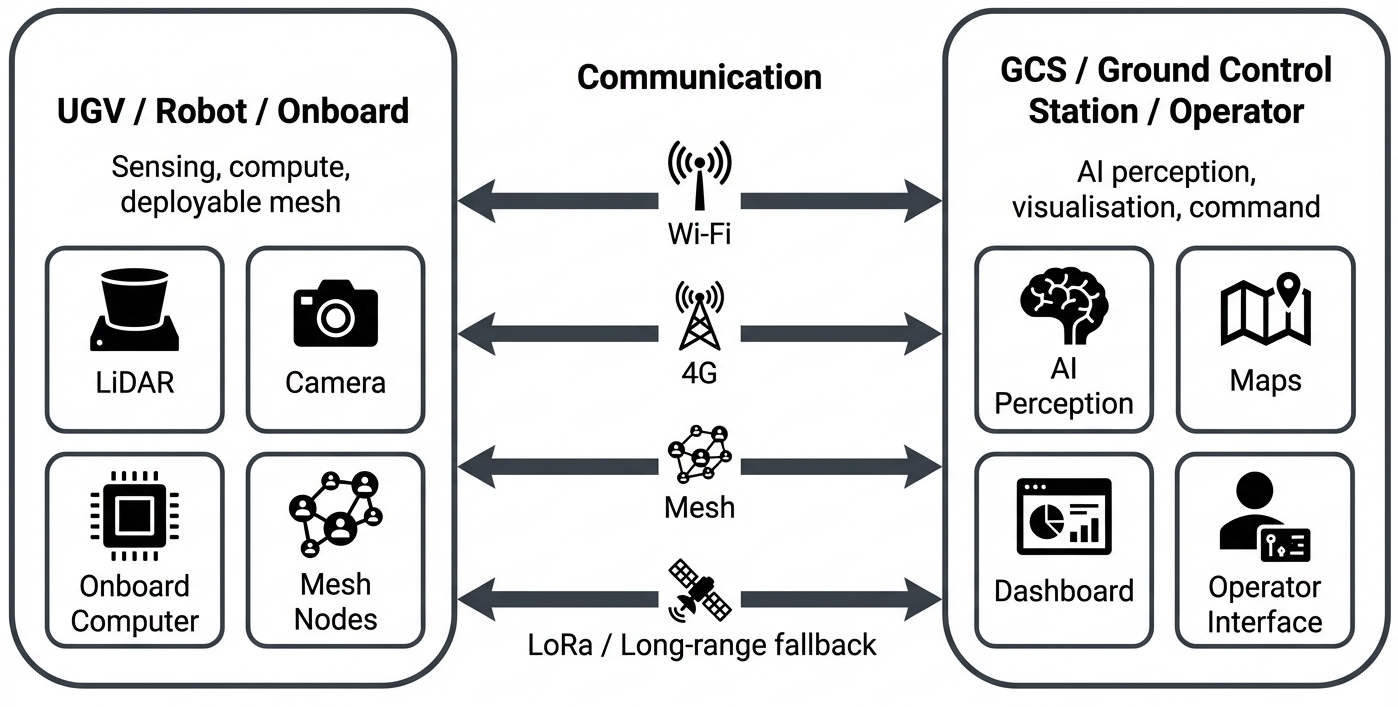
\includegraphics[width=0.8\textwidth]{figures/multitier_architecture.png}
\caption{Multi-tier system architecture for autonomous exploration with onboard sensing, mesh networking, and operator-side AI processing.}
\label{fig:multitier_arch}
\end{figure}

\section{Project Scope and Limitations}
\label{sec:scope}

The project focuses on indoor environments where GPS is unreliable, and LiDAR performs effectively without sunlight interference. A YDLidar X3 (10\,Hz) sensor supports 2D SLAM via Google Cartographer, generating 0.05\,m occupancy maps. The UGV autonomously explores with frontier-based algorithms while the Nav2 stack handles path planning and obstacle avoidance. The as-built system (Chapter~\ref{ch:impl}) covers an indoor test area of approximately 40$\times$30\,m, powered by a 24\,V pack (dual 3s3p 18650) with runtime of almost two hours at 0.2\,m/s.

A multi-tier communication framework combines ESP-WiFi-MESH as the core network with Wi-Fi, 4G, and LoRa (SX1278) as fallbacks. The UGV deploys compact mesh nodes (ESP32 DevKit, 2500\,mAh LiPo each) during exploration; nodes are added to the routing table upon deployment. AI-driven features include visual hazard detection (e.g.\ smoke, fire, extinguisher, human) and LLM-based summarisation for generating mission reports. Operators access a web dashboard offering live telemetry, map visualisation, video (720p, 15\,fps), detection overlays, and manual control. The software stack runs on ROS~2 Humble (Raspberry Pi~4 8\,GB) and ESP32 DevKit, demonstrating GPU-free autonomous operation.

The UGV handles flat surfaces with minor obstacles and supports payloads but cannot climb stairs or steep inclines. Its cameras (USB webcam and ESP32-CAM at 720p, 15\,fps) provide visual data only, lacking thermal or chemical sensing. Without wheel encoders, Cartographer's scan-matching combined with an MPU6050 IMU handles localisation, with reduced accuracy in feature-sparse spaces. The 2D SLAM system cannot detect overhead obstacles or elevation changes, limiting the robot to single-floor reconnaissance. AI inference runs on the ground station, requiring active connectivity for live overlays. These constraints were deliberately set to preserve project scope while achieving full autonomy and data processing from UGV to operator.

\section{Assumptions and Dependencies}
\label{sec:assumptions}

The study assumes that indoor disaster sites provide sufficient geometric features---walls, doors, and furniture---for reliable LiDAR-based localisation using Cartographer SLAM. Target environments are mostly intact buildings with traversable floors, emphasising floor-level hazard assessment. At least one active communication link within the multi-tier setup (mesh, Wi-Fi, 4G, LoRa) is expected during operations. The UGV's runtime (approximately two hours on the as-built pack) is considered adequate for the test coverage area at 0.2\,m/s, including a return margin.

AI perception is offloaded to the ground control station, maintaining low-latency detection through available bandwidth. The Raspberry Pi~4's quad-core CPU supports real-time Cartographer SLAM, Nav2 navigation, and sensor handling without requiring GPU-based systems. Mesh deployment assumes suitable node spacing for reliable indoor connectivity; SLAM corrections mitigate drift via loop closure. The system runs on ROS~2 Humble with Ubuntu 22.04 LTS for stability and long-term support. Cartographer depends on continuous 10\,Hz LiDAR input from the YDLidar X3 and proper TF tree configuration. Navigation uses Nav2 with tuned DWB planner parameters and costmap inflation. Communication resilience integrates ESP32 DevKit modules for ESP-WiFi-MESH, with 4G hotspot and SX1278 LoRa as fallback links. Power is supplied by a 24\,V pack (dual 3s3p 18650 in series) with appropriate regulation. Hardware components are sourced from available suppliers, with availability and pricing affecting system cost and timelines.

\section{Broader Impact (UN SDGs)}
\label{sec:sdg}

This project is directly motivated by two goals of the United Nations Sustainable Development Goals (SDGs): SDG~9 (Industry, Innovation, and Infrastructure) and SDG~11 (Sustainable Cities and Communities). The work can be used to develop resilient infrastructure and innovation in robotics; specifically, the decentralised communication in threat-affected environments by creating an autonomous Unmanned Ground Vehicle (UGV) that reacts to the crisis. Besides, the project should enhance the safety and sustainability of human settlements. This robotic system will improve rescue capability to save victims of disaster and catastrophic events since it is able to update the operators promptly on the prevailing information available concerning the situation of the disaster sufferers and the risky and unpredictable settings without endangering the rescuing team.

\section{Identified Core Challenges}
\label{sec:challenges}

Disaster-response UGVs face several core challenges. Accurate real-time SLAM is essential for navigation and spatial referencing, but practical issues such as sensor noise, wheel slip, and glass surface occlusions hinder mapping precision. Reliable multi-sensor data collection---camera, temperature, environmental---is equally important and requires deterministic acquisition with proper synchronisation and filtering to ensure usability.

Processing this data on embedded hardware remains difficult due to limited computational resources, often forcing offloading to cloud or operator systems. Communication in disaster zones is another constraint, as infrastructure is typically unavailable; while mesh networks provide resilience, they lack high throughput and suffer from attenuation and multipath fading.

The vast data influx also overwhelms human operators, creating cognitive strain and delays in decision-making. Automated interpretation through computer vision and LLMs can alleviate this but demands high power and computing capability, which impacts system cost, thermal performance, and battery life. Designing cost-effective, modular, and reusable systems is vital. The UGV should support additional payloads with minimal modifications, and mesh networks should remain interoperable across robots. Cooperative exploration through swarm robotics presents a promising approach to increase efficiency and mission coverage.

\section{Problem Statement}
\label{sec:problem}

Disaster-response operations require UGVs capable of autonomous navigation, localisation, communication, and perception to enhance mission efficiency and safety. Current systems often operate in isolation, struggling with real-time SLAM, data handling, and long-range communication due to hardware, power, and computational constraints. Limitations in embedded processing restrict advanced AI and mapping algorithms, while unreliable wireless links hinder operator connectivity. High design costs, low modularity, and poor interoperability further limit scalability.

This highlights the need for a resilient, efficient, and modular UGV platform that integrates SLAM, robust communication, and AI-driven data interpretation to enable reliable, scalable, and autonomous disaster-response missions.

\section{Thesis Outline}
\label{sec:outline}

This thesis is organised into six chapters detailing the design, implementation, and evaluation of an autonomous indoor exploration robot.

Chapter~1 has presented the project's motivation, objectives, and scope, outlining the disaster reconnaissance problem, system capabilities, and societal relevance with reference to the UN Sustainable Development Goals.

Chapter~2 reviews literature on autonomous robotics, SLAM, navigation, mesh networking, and AI perception, identifying research gaps that inform subsequent design choices.

Chapter~3 details the system architecture and design, including power and locomotion design, SLAM-based mapping, autonomous navigation, multi-tier communication, AI vision processing, and operator interface, supported by component-level trade-off analysis.

Chapter~4 describes hardware and software implementation and testing---covering integration, ROS~2 setup, network configuration, and interface development---along with unit and function testing.

Chapter~5 presents results of the development stages, comparison with design objectives and related work, and socio-economic and environmental impact.

Chapter~6 concludes with key contributions, lessons learned, and future directions such as 3D SLAM integration, multi-robot coordination, and deployment in varied operational scenarios. Appendices cover SDG mapping, source code structure, hardware schematics, bill of materials, and project timeline.

% Chapter 2: Literature Review (full)

\chapter{Literature Review}
\label{ch:lit}

The following review draws on foundational and recent work in exploration, SLAM, communication, and perception. Robotic search in collapsed, GNSS-denied indoor environments faces three core hurdles: reliable communication, localisation/autonomy, and real-time data delivery. While recent surveys show progress in perception and coordination, gaps remain in autonomy and interference \cite{queralta2020}. To avoid hazardous manual entry cycles, robots must balance autonomous exploration with consistent telemetry \cite{lu2022}. The sections below review existing technologies and their relevance to this study.

\section{Mapping and Localization}
\label{sec:lit_mapping}

LiDAR odometry is the most reliable mapping method indoors, as it is unaffected by lighting, smoke, or low-texture environments \cite{lee2024}. However, accuracy can diminish in repetitive corridors or sparse geometry without corrective algorithms. Consequently, it is standard to combine LiDAR with IMUs or visual odometry (VO), alongside scan-matching and loop closure, to reduce drift and maintain map consistency. These processes are computationally expensive for embedded systems with limited headroom. This trade-off between hardware and accuracy is central to developing realistic SLAM for disaster response. The goal is a cost-effective architecture balancing real-time SLAM, sensor fusion, localisation, and operator communication. Recent SLAM methods are compared in Table~\ref{tab:slam_compare}.

\begin{table}[htbp]
\caption{Comparison of scan-matching versus sensor fusion approaches for 2D SLAM in mobile robotics.}
\label{tab:slam_compare}
\centering
\small
\begin{tabular}{p{2.8cm}p{3.2cm}p{3.8cm}}
\toprule
\textbf{Aspect} & \textbf{ICP-Based 2D LiDAR \cite{silva2025}} & \textbf{Multi-Platform LIO/LO methods \cite{lee2024}} \\
\midrule
Sensor stack & Single 2D LiDAR with MPU6050 IMU (no wheel odometry), ICP-based scan-to-scan & LiDAR only / LiDAR-IMU / multi-LiDAR or optionally camera fusion \\
Core methodology & GN-ICP point-to-plane & LIO-SAM, FAST-LIO2, Point-LIO \\
Real-time & 3\,s delay due to ICP convergence on mini PC & High-rate odometry for aggressive motion \\
Loop closure & None & Present in many SLAM stacks \\
Key issue & ICP convergence time; localisation drifts over time & Needs accurate time-synced odometry and IMU data \\
\bottomrule
\end{tabular}
\end{table}

Combining aerial and ground robots is now standard in Search and Rescue (SAR) to maximise coverage and mobility, as seen in the DARPA Subterranean Challenge \cite{lu2022}. A case study of the NCTU team's heterogeneous system highlights key trade-offs: their autonomous blimp showed extreme stamina, using only 15.81\,W compared to a quadcopter's 971.9\,W. However, the blimp struggled in narrow tunnels ($<$2.5\,m) and moderate airflow, where drag overwhelmed propulsion. Its limited 86° field of view also led to frequent entrapments. Integrating data and maintaining SLAM consistency across such fleets is difficult. In the NCTU case, ground vehicles used Velodyne LiDAR with LeGo-LOAM, while the blimp used visual odometry; merging these disparate maps proved challenging. Power also remains a bottleneck. Consequently, for budget-constrained missions, a single optimised UGV can be more reliable than a complex heterogeneous fleet \cite{lu2022}.

Technically, ICP-based approaches are sensor-light but suffer from slow convergence and drift in featureless areas. Modern LiDAR-IMU Odometry (LIO) handles aggressive motion better but requires precise time-synchronisation and high-end computing. Many lightweight stacks also lack loop closure, leading to distorted maps during long missions. Indoor SAR presents unique hurdles like stairways, collapsed corridors, and smoke. While frontier-based exploration helps map unknown spaces, multi-storey navigation and localisation drift remain significant issues. Furthermore, most ICP systems assume static environments, but SAR sites contain dynamic obstacles that can degrade scan consistency. Without real-time filtering and robust sensor fusion (LiDAR, IMU, and wheel odometry), maps can deteriorate rapidly. In conclusion, a bottleneck persists due to the lack of embedded-ready, integrated SLAM stacks. Practical solutions must optimise for limited hardware while ensuring resilience in dynamic environments and consistent loop closure.

\section{Communication and Networking}
\label{sec:lit_comms}

Indoor wireless networking faces severe constraints in SAR due to walls and debris causing attenuation, fading, and congestion \cite{matracia2022}. Consequently, exploration systems must be self-forming and self-healing. A hybrid approach is preferred: high-rate channels (Wi-Fi/5G) for video and maps, paired with a reliable low-rate link for telemetry and control. Since indoor geometry often blocks line-of-sight for aerial relays, grounded robots and static nodes are prioritised to maintain data paths to command posts. Table~\ref{tab:comms_compare} compares wireless communication approaches for disaster site robot networks.

\begin{table}[htbp]
\caption{Comparison of wireless communication approaches for disaster site robot networks.}
\label{tab:comms_compare}
\centering
\small
\begin{tabular}{p{1.8cm}p{1.6cm}p{2.2cm}p{2.2cm}p{2cm}}
\toprule
\textbf{Work} & \textbf{Goal} & \textbf{Strengths} & \textbf{Issues} & \textbf{Key metrics} \\
\midrule
SDR UAV \cite{rukaiya2024} & Hybrid UAV connectivity & Virtual sub-networks, parallel links & Assumes LoS; indoor multipath severe & 2.6\,Mb/s; latency 340--820\,ms \\
6G/SAGIN \cite{matracia2022} & Survey recovery comms & DTN, SDN, UAV placement, backhaul & No implementations; few indoor models & Coverage/capacity; handover \\
LoRa indoor/outdoor \cite{saban2021} & LoRa RSSI/SNR/PDR & Empirical attenuation; gateway elevation & Low throughput; high latency; no mesh & PDR $<$40\% at 2 walls; 0.25--5.4\,kbps \\
Mobile relay \cite{hurst2023} & Robotic relay optimisation & Joint stop positions + routing; handles non-convex & Single relay; simulation-only & $\sim$35\% lower wait vs TSP; $\sim$50\,m/link \\
\bottomrule
\end{tabular}
\end{table}

LoRa is often unsuitable for multi-robot coordination in debris-filled buildings, as packet delivery rates can drop below 40\% after only a few structures \cite{saban2021}. Instead, 2.4\,GHz mesh architectures are preferred for their ability to adaptively route through relays. Modern SAR robots increasingly use communication-aware navigation, treating link quality (RSSI and SNR) as a core operational input. Mobile relays can improve wait times when stop locations are optimised for signal strength \cite{hurst2023}. The NCTU team addressed indoor constraints using a three-tier mesh architecture \cite{lu2022}: XBee (ZigBee) for low-bandwidth control and telemetry (indoor range 25--75\,m for $\sim$85\% PDR, with 90° corners causing 15--20\,dB losses); UWB for ranging (7--13\,m reliable, single turns 15--33\,dB losses); WiFi mesh for map sync and video (1--4 FPS), with PDR highly volatile (20--80\%) based on antenna or geometry. These findings highlight that autonomous SAR agents cannot rely on static network planning and instead require navigation models that dynamically balance exploration goals with signal thresholds for node dispersal \cite{lu2022}.

\section{Human-Robot Collaboration}
\label{sec:lit_hri}

SAR research focuses on three themes: computational efficiency for hardware-constrained mapping, resilient communication to handle network disruptions, and intuitive human-robot interaction to reduce responder cognitive load. Despite progress in system frameworks and path-blocking strategies, current solutions remain fragmented. Most work is either high-level conceptual framing or highly specialised studies on specific navigation or aerial supervision pipelines. Consequently, there is a lack of practical, integrated ground-robot systems that combine mapping, networking, and collaboration into a single deployable platform \cite{queralta2020}. Table~\ref{tab:hri_compare} compares existing HRI methods in SAR, including clearance-aware path planning \cite{lee2023} and multi-robot operator supervision \cite{chan2023}.

\begin{table}[htbp]
\caption{Comparison of existing HRI methods in SAR.}
\label{tab:hri_compare}
\centering
\small
\begin{tabular}{p{2.2cm}p{2.2cm}p{2.2cm}p{1.8cm}p{2.2cm}}
\toprule
\textbf{Domain} & \textbf{Approach} & \textbf{Results} & \textbf{Key metrics} & \textbf{Limitations} \\
\midrule
Multi-robot SAR \cite{queralta2020} & Conceptual architectures (planning, coordination, perception) & Autonomy, communication, coordination challenges & Mostly conceptual & Heavy focus on swarms; lacks embedded feasibility \\
Indoor path planning \cite{lee2023} & Clearance-aware multi-level route optimisation & Efficient path computation & Faster pathfinding in simulation & Focused on human rescuers; no comm or AI \\
HRI \cite{chan2023} & Operator supervising multiple robots; real-time mapping and object detection & Intuitive interfaces; reduced operator load in GNSS-denied & Indoor trials; real-time image streaming & UAV-focused; multiple aerial robots; high-end hardware \\
\bottomrule
\end{tabular}
\end{table}

Research shows that progress in SAR robotics remains siloed. Conceptual frameworks define high-level needs but rarely translate into embedded, cost-constrained ground platforms. While indoor path planning achieves efficiency and human-intuitive routing, it often lacks the communication resilience and perception layers essential for debris-filled environments. Similarly, human-robot collaboration studies demonstrate intuitive interfaces that reduce operator workload, but these are largely limited to UAV fleets in controlled settings using expensive hardware and stable networks.

\section{AI-Based Perception}
\label{sec:lit_ai}

AI for SAR perception focuses on converting raw sensor data into actionable insights. Immersive 3D mapping uses LiDAR-SLAM and hazard sensing to create real-time VR/AR reconstructions; field tests show such systems can fly for 16 minutes at 1--5\,m/s while identifying shielded radiation sources \cite{dayani2021}. Other approaches utilise video foundation models to summarise robot footage into storyboards or text summaries \cite{video2023}; query-driven summarisation achieves high accuracy and saves operators time compared to raw video, but high GPU requirements and 9--23\,s latencies hinder real-time deployment. Similarly, LLMs can translate egocentric metadata into natural-language reports or temporal queries \cite{dechant2023}; while QA accuracy is high in familiar settings, summary accuracy drops in unseen environments. Most of these methods rely on simulations and lack stress-testing against noisy, real-world SAR data. Table~\ref{tab:ai_compare} compares existing work on AI perception in robots.

\begin{table}[htbp]
\caption{Comparison of existing work on AI perception in robots.}
\label{tab:ai_compare}
\centering
\small
\begin{tabular}{p{2.2cm}p{2cm}p{2cm}p{2.2cm}p{2.2cm}}
\toprule
\textbf{Domain} & \textbf{Robot/sensing} & \textbf{Algorithm} & \textbf{Key metrics} & \textbf{Gaps} \\
\midrule
3D mapping + hazard \cite{dayani2021} & Single aerial; LiDAR + sensors & Real-time SLAM + reconstruction & $\sim$16\,min @ 6\,kg; 1--5\,m/s; localised source & Single platform; no coordination \\
Video summarisation \cite{video2023} & Multi-robot egocentric video & Video embeddings + temporal segmentation & Query accuracy high; storyboard saves $\sim$125\,s; latency 9--23\,s & Latency; GPU; domain shift \\
Language action \cite{dechant2023} & Virtual agents; egocentric data & CNN+LLM for QA + summarisation & QA acc 0.99 (seen); long-summary 0.85 (seen) & Sim-to-real gap; poor generalisation \\
\bottomrule
\end{tabular}
\end{table}

The gap between laboratory performance and SAR operational reality is vast. Using data from the DARPA SubT Challenge, the NCTU group evaluated CNN architectures (FCN, Mask-RCNN, Yolact) on NVIDIA Jetson Xavier in smoky tunnels \cite{lu2022}. Their findings reveal a critical trade-off: Mask-RCNN provided high precision (up to 0.770 AP) but operated at only 1.0 FPS; faster models like Yolact (2.4 FPS) suffered from extreme noise sensitivity, with accuracy dropping to near zero in cluttered underground conditions \cite{lu2022}. General-purpose CNNs on budget hardware necessitate significant trade-offs. For resource-constrained SAR systems, specialised detection pipelines may be more reliable than broad deep-learning models \cite{lu2022}. While individual fields like LiDAR-IMU odometry, mesh networking, and HRI have advanced, they remain isolated; high-performance solutions often require hardware or bandwidth currently unavailable to deployable ground robots \cite{lee2024}.

Field results from the SubT Challenge highlight a disconnect between theory and practice. High-accuracy LiDAR-IMU odometry demands compute power exceeding embedded limits, while lightweight ICP-based alternatives suffer from significant drift \cite{lu2022}. Communication also remains a dominant bottleneck. Furthermore, current systems often lack communication-aware navigation, where paths are planned based on real-time signal strength. Despite advances in decentralised coordination, the human-on-the-loop model remains essential. This bottleneck is mirrored in AI perception, where the compute cost of high-fidelity models restricts their real-world utility on embedded chips. While heterogeneous fleets offer conceptual advantages, coordination overhead and physical vulnerabilities often make robust, single-platform ground systems more practical in actual disaster scenarios.

Lu et al.\ \cite{lu2022} provide a strong methodological foundation but expose key gaps in human-robot interaction and embedded algorithm deployment. Their system relies heavily on human supervision for goal setting and data interpretation. Our project addresses this through automated reporting that converts sensor data into natural-language summaries and actionable insights, significantly reducing cognitive load. Although Lu et al.\ employ advanced algorithms, their reliance on high-end hardware such as NVIDIA Jetson and industrial PCs overlooks power constraints. In contrast, our solution runs on a Raspberry Pi~4 and embedded microcontrollers, achieving lower energy use, extended runtimes, and cost-effective deployment. Their research, tailored for the DARPA SubT Challenge, focuses on specialised systems like blimps and mmWave radar for subterranean exploration. Our project instead targets accessible surface environments with lightweight, deployable hardware. Finally, while their relay nodes offer temporary mesh coverage, our long-duration mesh nodes (added to the routing table upon deployment) provide persistent, reusable communication infrastructure, enabling sustained operation and supporting multi-robot collaboration.

% Chapter 3: Methodology and System Design (full)
% As-built specs (paper): 0.2 m/s, ~2 h runtime, 3-5 min init, MPU6050 IMU, no wheel odometry, ESP32 DevKit, 720p 15 fps, custom frontier + ProxMaP.

\chapter{Methodology and System Design}
\label{ch:method}

\section{Conceptual Framework}
\label{sec:conceptual}

The system utilises a multi-tier autonomous exploration architecture to balance real-time control with the heavy computational demands of AI vision. It is built on three core principles: onboard autonomy for network-independent traversal, multi-level networking (Wi-Fi, 4G, and mesh) with graceful fallback for resilient operator contact, and distributed processing to offload intensive AI tasks to the ground control station. The technological framework integrates ROS~2 \cite{ros2humble} for middleware and sensor fusion, using Google's Cartographer \cite{hess2016} for SLAM to generate 2D occupancy grids. These maps inform the Nav2 stack \cite{nav2dwb} for cost-aware path planning. For communication, the ESP-WiFi-MESH framework \cite{espmesh} enables the UGV to deploy persistent mesh nodes along its path, while 4G hotspot and LoRa provide fallbacks. Finally, an AI perception pipeline on the GCS processes camera feeds to generate actionable mission reports.

\section{High-Level Design}
\label{sec:hld}

Figure~\ref{fig:system_topo} illustrates that the system architecture comprises three primary domains interconnected by a multi-mode communication network. The Unmanned Ground Vehicle (UGV) subsystem combines computing, perception, and locomotion control into a mobile platform that recognises novel surroundings through autonomous navigation. The communication system is constituted by multiple connection modes: ESP-WiFi-MESH as the primary mesh, direct Wi-Fi, 4G cellular, and LoRa at 433\,MHz for resilience and emergency command. All AI perception pipeline, web-based operator dashboard, and mission management interfaces reside at the Ground Control Station (GCS). The two-way data flow allows telemetry and video to be transmitted from the UGV to the GCS, and navigation orders and AI detection results to be sent to the UGV.

% --- FIGURE: System topology ---
\begin{figure}[htbp]
\centering
\includegraphics[width=0.85\textwidth]{figures/system_topology.png}
\caption{System topology and data flow diagram.}
\label{fig:system_topo}
\end{figure}

The operational cycle begins with system initiation (3--5 minutes): the battery system is enabled and the Raspberry Pi~4 boots Ubuntu 22.04 and ROS~2 \cite{ros2humble}. Sensor drivers activate the YDLidar X3 \cite{ydlidar} at 10\,Hz, the MPU6050 IMU, and the cameras at 720p, 15\,fps; the mesh and Wi-Fi/4G links come up. A WebSocket-based web interface at the GCS displays initial diagnostics, including battery voltage, network status, and sensor health. Cartographer SLAM \cite{hess2016} processes LiDAR scans and IMU data (scan-matching and loop closure; no wheel odometry) to generate a 2D occupancy grid. Map updates are transmitted to the GCS for operator monitoring. The Nav2 stack \cite{nav2dwb} uses global and local costmaps for path planning, with the DWB local planner translating velocities into wheel commands. Autonomous exploration is driven by a custom frontier-based method \cite{yamauchi1997} that identifies frontiers, ranks them (including with ProxMaP-style AI map prediction \cite{sharma2022}), and sends goals to Nav2. The cycle continues until coverage is complete or the operator terminates the mission. For perception, video is streamed to the GCS; the operator-side AI runs YOLOv8 detectors and an LLM for scene and hazard analysis, with spatial decision memory (X-SDM) and person profiling. Telemetry is sent at a steady rate. The communication layer switches between mesh, Wi-Fi, and 4G, with LoRa serving as a low-bandwidth fallback for telemetry and return-to-base. The mission concludes when exploration is complete or the battery reaches a safety threshold; the robot can return to base using the recorded map.

\section{Subsystem Design}
\label{sec:subsystem}

\subsection{Power System Design}
\label{sec:power}

The power system provides 24\,V nominal voltage using a modular dual 18650 lithium-ion battery setup. The architecture consists of two 3s3p packs in series, each delivering 11.1\,V nominally (12.6\,V peak), with the series combination giving nominal 22.2--24\,V. Each pack is managed by a BMS providing overvoltage, undervoltage, and overcurrent protection. Usable energy is limited to a safe depth-of-discharge, providing sufficient capacity for almost two hours of continuous operation at 0.2\,m/s in the as-built system. The 24\,V output bifurcates: the high-power branch supplies unregulated voltage to the motor drivers; the low-power branch uses a buck converter to provide a regulated 5\,V rail for the Raspberry Pi~4, sensors (LiDAR, Kinect v1, USB webcam), ESP32-CAM, router, and headlights. The deployable mesh nodes are each powered by a 2500\,mAh LiPo.

% --- FIGURE: Power distribution ---
\begin{figure}[htbp]
\centering
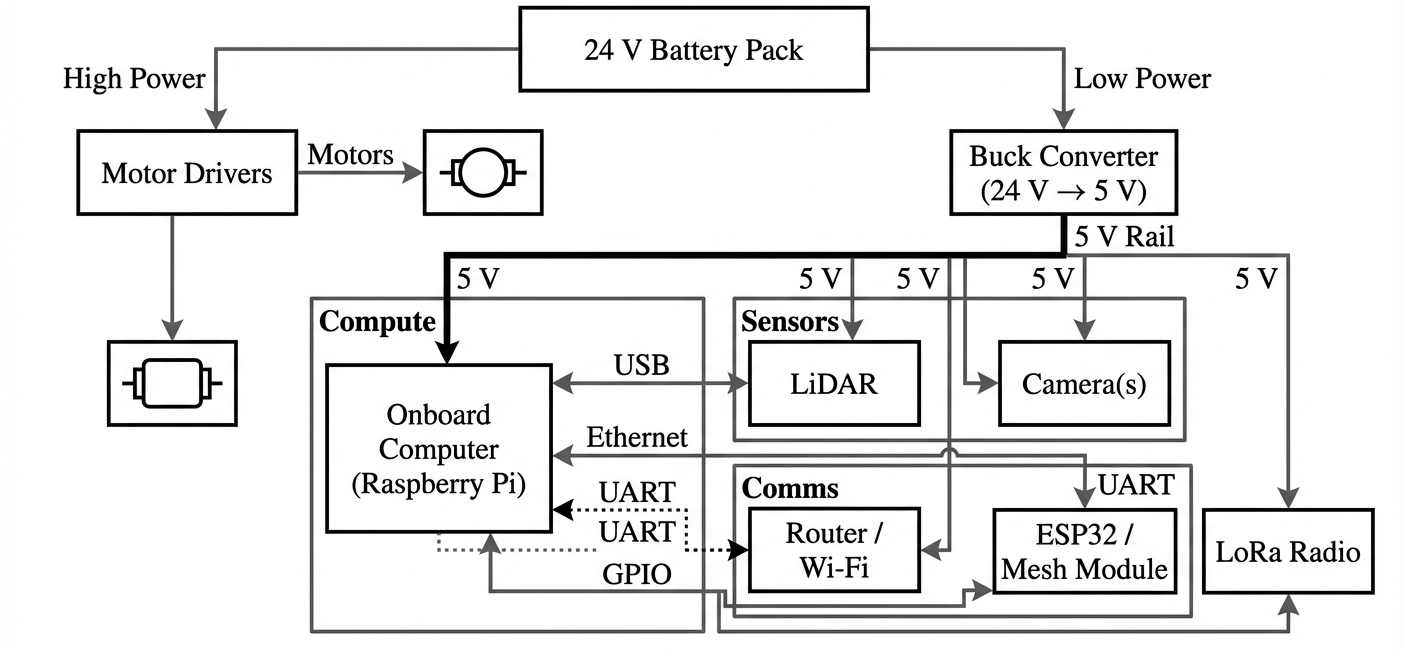
\includegraphics[width=0.7\textwidth]{figures/power_diagram.png}
\caption{Power distribution diagram.}
\label{fig:power_dist}
\end{figure}

\subsection{Locomotion and Control}
\label{sec:locomotion}

The locomotion system uses a 4WD chassis with skid-steering for mobility in cluttered environments. The chassis balances stability and manoeuvrability, allowing passage through standard doorways while maintaining a low centre of gravity. Skid-steering operates on differential-drive principles: left and right wheel pairs are driven independently; forward motion is achieved by matching side speeds, and turning from velocity differences. In-place rotation is possible by counter-rotating the sides. The platform is designed for relatively flat indoor terrain; steep slopes, large rubble, and staircases are outside its operational scope. The system intentionally omits motor encoders, relying solely on Cartographer's scan-matching for localisation. This reduces hardware complexity and cost. To keep scan-matching reliable, autonomous speed is capped at 0.2\,m/s; at 10\,Hz LiDAR, the robot travels 20\,mm between scans, ensuring strong feature overlap. Locomotion is optimised for partially intact indoor buildings, with the ability to clear minor obstacles such as doorsteps or cables. The control architecture uses an ESP32 (or equivalent) as an intermediary between the Raspberry Pi~4 and the motor drivers where appropriate; velocity commands from Nav2 are published to \texttt{/cmd\_vel} and converted to motor outputs.

% --- FIGURE: Chassis dimensions ---
\begin{figure}[htbp]
\centering
\includegraphics[width=0.6\textwidth]{figures/chassis_dimensions.png}
\caption{Planned dimensions of the UGV chassis.}
\label{fig:chassis}
\end{figure}

The motor driver and configuration are shown in Figure~\ref{fig:motor_config}.
\begin{figure}[htbp]
\centering
\includegraphics[width=0.6\textwidth]{figures/motor_config.png}
\caption{Motor configuration and drive interface.}
\label{fig:motor_config}
\end{figure}

\subsection{Perception and Mapping}
\label{sec:perception_mapping}

The perception and mapping subsystem provides real-time localisation and map generation. The system uses a YDLidar X3 2D laser scanner: 360° range 0.12--12\,m, 10\,Hz scan rate, approximately 1° angular resolution. It connects to the Raspberry Pi~4 via USB--UART. A Microsoft Kinect v1 is used as an RGB-D camera under budget constraints; its point cloud is fused into the Nav2 local costmap to improve obstacle avoidance for overhangs and table legs. Vision for the operator is provided by a USB webcam (main) and an ESP32-CAM (rear), both at 720p and 15\,fps \cite{ydlidar}.

Google Cartographer serves as the SLAM framework, using graph-based optimisation to estimate robot poses and create 2D occupancy grids \cite{hess2016}. The algorithm maintains a pose graph; when the robot returns to a previously visited area, Cartographer performs loop closure to eliminate cumulative drift. Cartographer was selected for its robust approach, allowing accurate positioning from LiDAR data and the MPU6050 IMU, without requiring wheel encoders. The framework uses a hierarchical submap approach; real-time scans are matched against submaps to build the grid. The system uses an occupancy grid resolution of 0.05\,m (5\,cm). The software platform is Ubuntu 22.04 LTS running ROS~2 Humble \cite{ros2humble}. The Raspberry Pi~4 (8\,GB RAM) provides the necessary processing for Cartographer at 10\,Hz. The coordinate frame architecture follows ROS~2 conventions: the map--odom--base\_link--laser\_link transform chain; Cartographer publishes map$\to$odom to correct drift. The laser frame is set with a static offset from base\_link for accurate spatial projection. Loop closure reduces drift to under approximately 5\,cm in feature-rich regions; in feature-poor areas drift can reach approximately 20--30\,cm until a distinctive feature is revisited. Figure~\ref{fig:carto_posegraph} shows the Cartographer pose graph and loop closure; the TF coordinate frame tree is illustrated in Figure~\ref{fig:tf_tree}. Limitations include inability to detect obstacles outside the LiDAR plane (e.g.\ overhanging cables) and sensitivity to glass; these are accepted for floor-level reconnaissance.

% --- FIGURE: Cartographer pose graph ---
\begin{figure}[htbp]
\centering
\includegraphics[width=0.75\textwidth]{figures/carto_posegraph.jpg}
\caption{Cartographer pose graph and loop closure.}
\label{fig:carto_posegraph}
\end{figure}

\begin{figure}[htbp]
\centering
\includegraphics[width=0.7\textwidth]{figures/tf_tree.jpg}
\caption{TF coordinate frame tree (map, odom, base\_link, laser).}
\label{fig:tf_tree}
\end{figure}

% --- FIGURE: Occupancy grid ---
\begin{figure}[htbp]
\centering
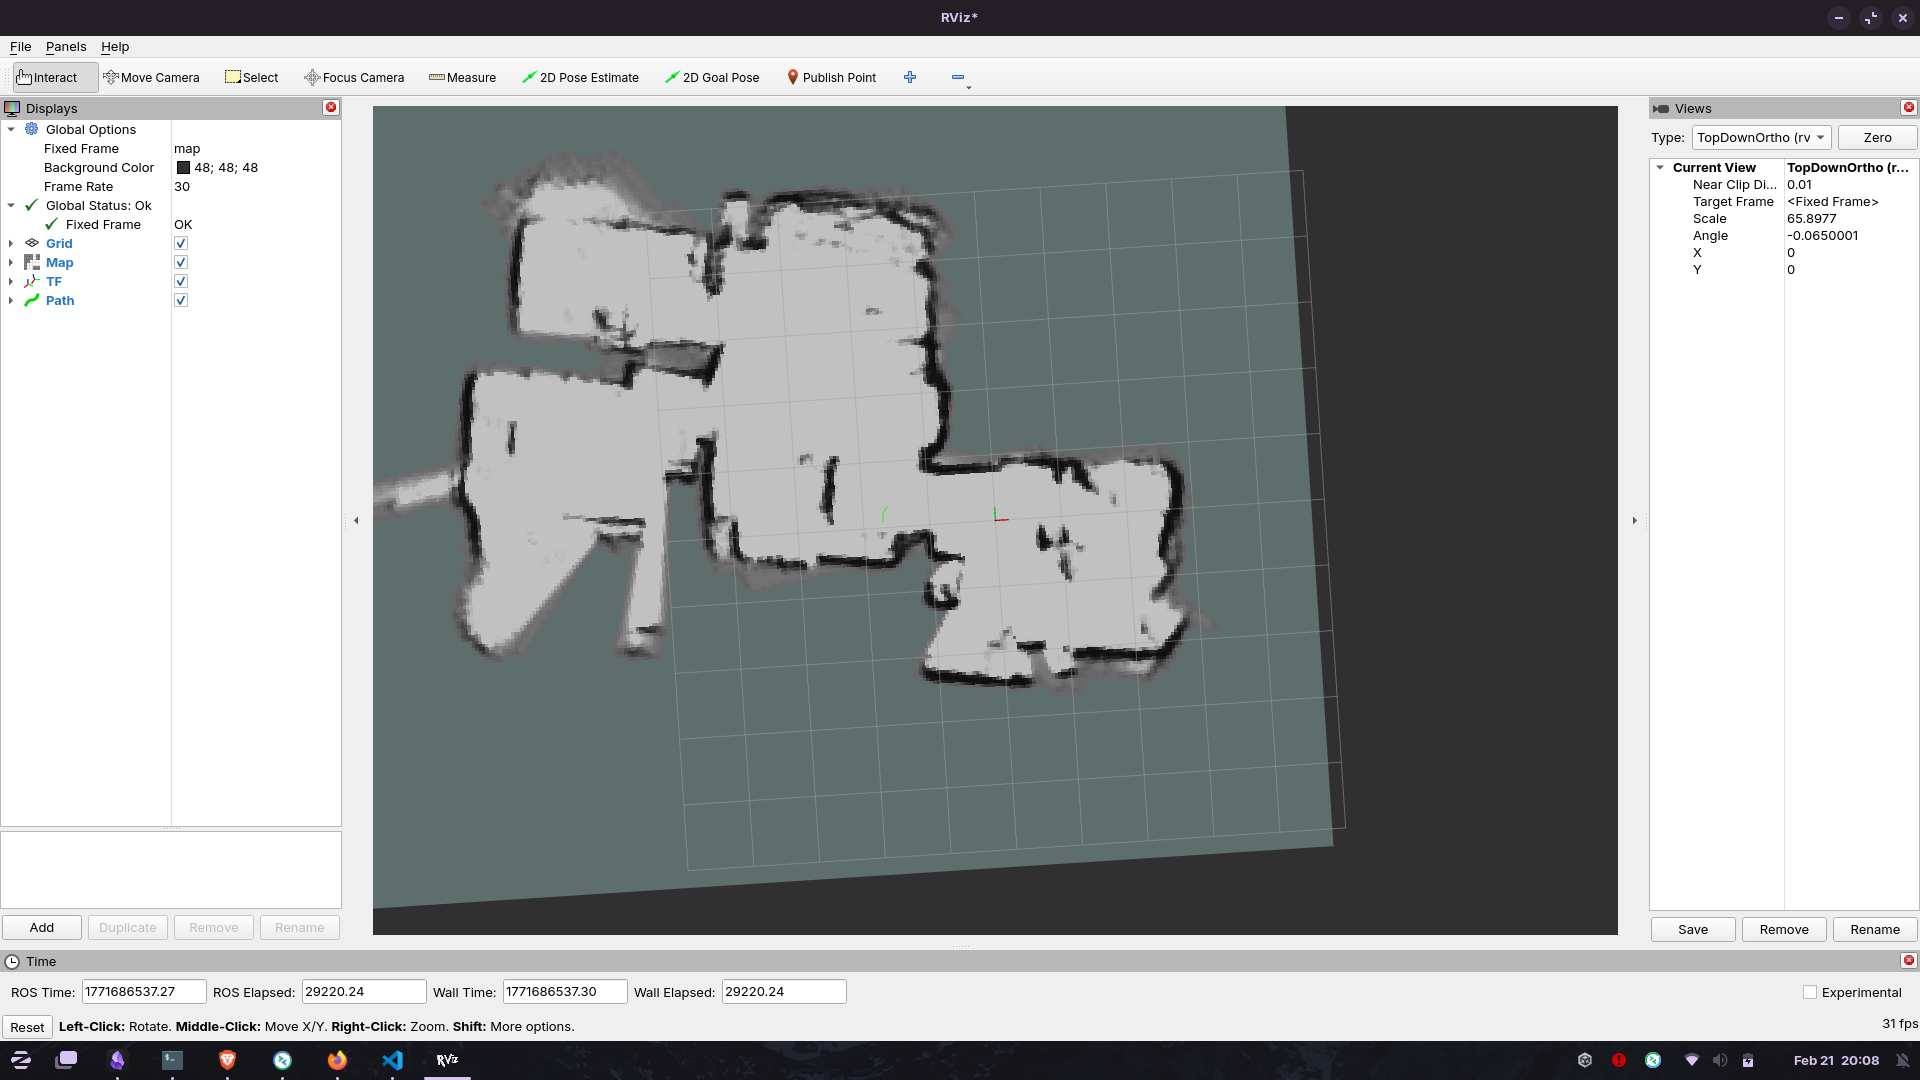
\includegraphics[width=0.75\textwidth]{figures/occupancy_grid.png}
\caption{Occupancy grid generated by SLAM.}
\label{fig:occupancy_grid}
\end{figure}

\subsection{Navigation and Autonomous Exploration}
\label{sec:nav_explore}

The navigation and autonomous exploration subsystem converts SLAM occupancy grids into robot motion. The system uses the ROS~2 Navigation Stack (Nav2): global path planning, local trajectory optimisation (DWB controller), and costmap management. Nav2 processes the Cartographer grid and pose to compute collision-free paths and publishes velocity commands to \texttt{/cmd\_vel}. The global planner uses Dijkstra's algorithm on the occupancy grid \cite{rachmawati2020}; the local planner uses the Dynamic Window Approach (DWB) \cite{nav2dwb} for obstacle avoidance and smooth trajectories \cite{gomez2024}. Costmaps combine a static layer from SLAM, an obstacle layer (LiDAR and Kinect v1 point cloud in the local costmap), and an inflation layer (0.3\,m safety margin). The global costmap uses the full grid and updates at a moderate rate; the local costmap maintains a rolling window around the robot for real-time obstacle reaction. Figure~\ref{fig:nav2_costmap} shows the Nav2 local costmap and obstacle layer.

\begin{figure}[htbp]
\centering
\includegraphics[width=0.8\textwidth]{figures/nav2_costmap.png}
\caption{Nav2 local costmap and obstacle layer.}
\label{fig:nav2_costmap}
\end{figure}

Autonomous exploration is handled by a custom-built frontier-based package that integrates with Nav2 \cite{yamauchi1997}. Frontier cells are free cells with at least one unknown neighbour (a 5$\times$5 window handles Cartographer's border). Frontiers are clustered with 8-connected BFS and scored using a linear combination of spatial and heuristic factors:
\begin{equation}
Score(f_i) = \alpha \cdot G(f_i) + \beta \cdot H(f_i) + \gamma \cdot I_{AI}(f_i) - \delta \cdot D(x_r, f_i)
\label{eq:frontier_score}
\end{equation}
where $G(f_i)$ is the grid cluster size of the $i$-th frontier, $H(f_i)$ is the heading bonus prioritising forward-facing exploration, $I_{AI}(f_i)$ is the AI map-prediction information gain, $D(x_r, f_i)$ is the Dijkstra path distance from the current robot pose $x_r$, and the Greek letters represent empirically tuned constraint weights. Figure~\ref{fig:detected_frontiers} shows detected frontier cells and clustering. The AI map-prediction layer defining $I_{AI}(f_i)$ runs a ProxMaP U-Net \cite{sharma2022} on a $128\times128$ robot-centred map crop. The network accepts a two-channel input (normalised occupancy and an unknown-cell mask) and outputs three-class logits (free, occupied, unknown). It was trained self-supervised on approximately 6\,000 map pairs from the AI2THOR simulator \cite{sharma2022}, achieving 85.43\% prediction accuracy and an F1 score of 87.42\% on the occupied class. In the original study, the predictor improved navigation efficiency by 12.4\% (SCT metric) over a non-predictive baseline. In our system the predicted map boosts the score of frontiers bound for open space, effectively reducing backtracking. The explorer supports dynamic replanning and manual no-go zones via RViz. Recovery behaviours include rotate-in-place, back-up, and costmap clearing. Exploration terminates when no frontiers remain, when battery reaches a configurable minimum (return-to-base), or when the operator aborts. Teleoperation override is supported: control inputs from the GCS override autonomous commands; when manual input ceases, the system resumes exploration.

% --- FIGURE: Detected frontiers ---
\begin{figure}[htbp]
\centering
\includegraphics[width=0.75\textwidth]{figures/detected_frontiers.jpg}
\caption{Detected frontier cells and clustering.}
\label{fig:detected_frontiers}
\end{figure}

The global planner computes shortest paths on the occupancy grid using Dijkstra's algorithm; the path is computed on the discrete grid and then followed by the local planner. When an obstacle appears in the planned path (for example when the LiDAR or Kinect detects a new obstacle), the costmap is updated and the path is recomputed. Figure~\ref{fig:nav_paths} shows a typical Dijkstra path and the path before and after obstacle replanning.

\begin{figure}[t]
\centering
\includegraphics[width=0.72\textwidth]{figures/dijkstra_path.jpg}\\[6pt]
\begin{minipage}[t]{0.48\textwidth}
\centering
\includegraphics[width=\linewidth]{figures/path_before_obstacle.png}\\
(a) Before obstacle detection
\end{minipage}\hfill
\begin{minipage}[t]{0.48\textwidth}
\centering
\includegraphics[width=\linewidth]{figures/path_after_obstacle.png}\\
(b) After replanning
\end{minipage}
\caption{Navigation path planning: Dijkstra pathfinding (top); path before and after obstacle detection (bottom).}
\label{fig:nav_paths}
\end{figure}

The local planner (DWB) tracks the global path while avoiding obstacles. Once the obstacle is incorporated into the local costmap, Nav2 replans and the robot follows an updated path that avoids the obstacle. This behaviour ensures that exploration continues safely even when the environment changes during a run.

\clearpage
\subsection{Communication and Network Architecture}
\label{sec:comms_design}

The communication subsystem offers robust connectivity between the UGV and GCS. The architecture uses four redundant technologies: ESP-WiFi-MESH \cite{espmesh} for extended multi-hop routing, direct Wi-Fi for high-bandwidth local transfer, 4G cellular when Wi-Fi is out of range, and 433\,MHz LoRa (SX1278) as a low-bandwidth emergency backup. These modes are managed so that high-performance links are preferred while lower-bandwidth channels remain as fallbacks.

Rather than treating each outage independently, the design follows an ordered degradation policy. The active tier advances from Wi-Fi (full video, map, and control traffic) to 4G when the local Wi-Fi path fails sustained health checks, then to ESP mesh with compressed imagery and reduced map update rates, and finally to LoRa for essential telemetry and safety-related commands when no IP backhaul is available. Downgrades use relatively short timeouts so the operator is not left on a dead link; recovery to a higher tier is gated by longer stable-good intervals (hysteresis) to avoid oscillation at building boundaries. Figure~\ref{fig:state_diagram} summarises this state-oriented view alongside the physical topology in Figure~\ref{fig:network_topo}.

\begin{figure}[htbp]
\centering
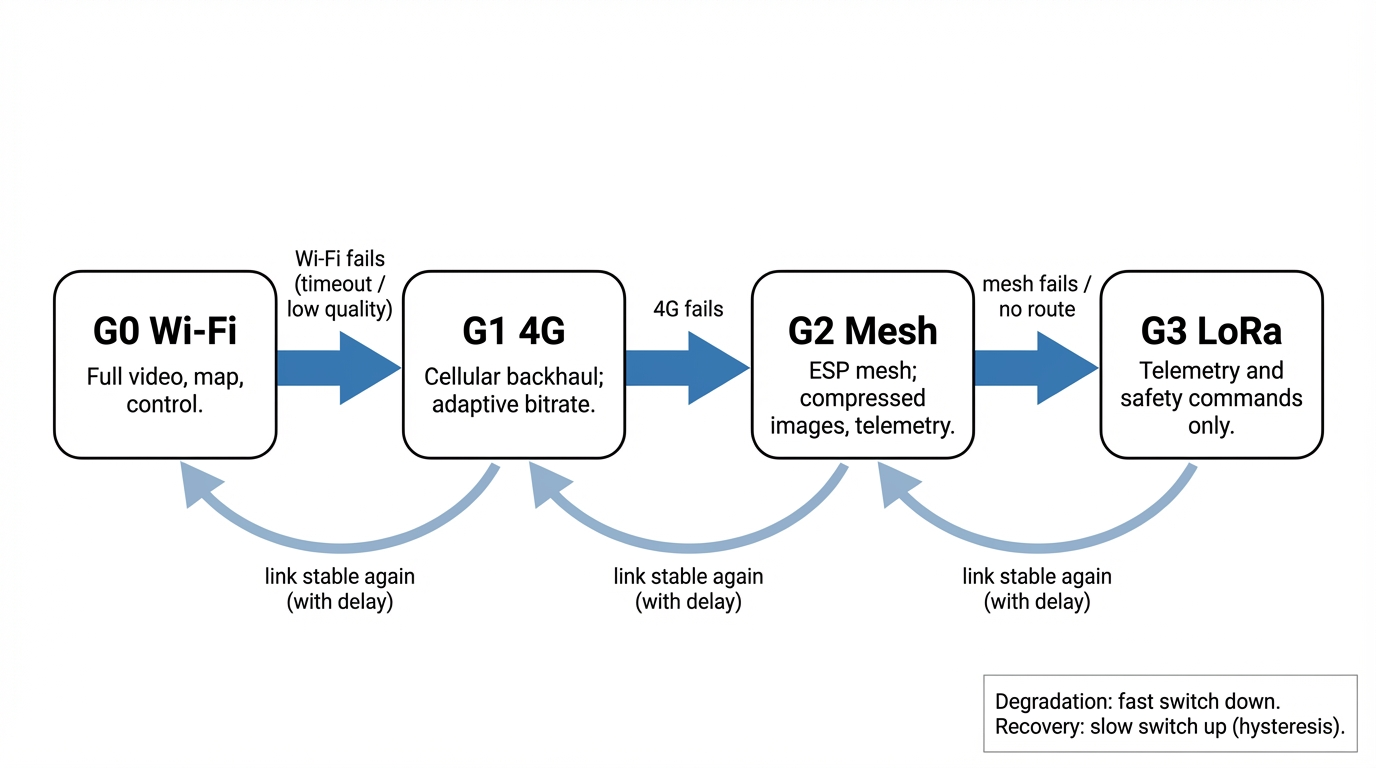
\includegraphics[width=0.92\textwidth]{figures/state_diagram.jpeg}
\caption{Network degradation state machine: preferred progression Wi-Fi $\rightarrow$ 4G $\rightarrow$ mesh $\rightarrow$ LoRa, with slower upgrade paths to limit link flapping.}
\label{fig:state_diagram}
\end{figure}

The backbone uses ESP-WiFi-MESH on ESP32 DevKit microcontrollers \cite{espmesh}. The UGV deploys up to two nodes along its path via a servo mechanism. To ensure a resilient connection pipeline without saturating the environment, the autonomous deployment trigger is dictated by a threshold function evaluating wireless link quality constraints:
\begin{equation}
D_{trigger} = 
\begin{cases} 
1, & \textbf{if } \text{RSSI}_{avg}(t) < -80\,\text{dBm} \text{ for } \Delta t \ge 3\,\text{s} \\
1, & \textbf{if } \text{PDR} < 85\% \\
0, & \textbf{otherwise}
\end{cases}
\label{eq:mesh_deployment}
\end{equation}
where $\text{RSSI}_{avg}$ is the moving average of the received signal strength indicator and $\text{PDR}$ is the real-time packet delivery ratio. Once triggered ($D_{trigger} = 1$), the node is released and automatically added to the active routing table. Nodes are powered by a 2500\,mAh LiPo each. When only mesh is available, images are iteratively WebP-compressed to a strict 8\,kB limit, Base64-encoded, and reconstructed at the operator side. Direct Wi-Fi (e.g.\ TP-Link Archer C6 on UGV, Tenda F3 at GCS) provides high bandwidth when the UGV is within range; throughput drops with walls and distance. The 4G hotspot provides wide-area connectivity when Wi-Fi is unavailable. The LoRa SX1278 link carries critical telemetry (position, battery, status) and emergency commands (e.g.\ return-to-base) when other links fail. The multi-tier design ensures graceful degradation from real-time video to periodic images to text-only telemetry.

% --- FIGURE: Network topology ---
\begin{figure}[htbp]
\centering
\includegraphics[width=0.8\textwidth]{figures/network_topology.jpg}
\caption{Network topology diagram.}
\label{fig:network_topo}
\end{figure}

\subsection{Vision and AI Perception}
\label{sec:vision_ai}

The vision and AI perception subsystem includes real-time object detection, LLM-based scene understanding, spatial decision memory (X-SDM), and mission logging. The visual system uses a USB webcam (main) and an ESP32-CAM (rear), both at 720p and 15\,fps. Video is streamed over the main link when Wi-Fi or 4G is available; on link degradation, images are sent over the mesh. AI perception is offloaded to the operator workstation to preserve the UGV's power budget and to leverage GPUs for fast inference.

The detection pipeline runs three YOLOv8m \cite{jocher2023yolov8} models (25.9M parameters each) in parallel: a fire/smoke detector fine-tuned on the Kerby Fire/Smoke dataset \cite{kerby2024firesmoke} (approximately 11\,000 images, two classes), a human detector using the default COCO pre-trained person class (class~0), and an extinguisher detector fine-tuned on the Roboflow FireExtinguisher dataset \cite{fireextinguisher2022roboflow} (3\,300 images, eight classes). Confidence thresholds are set to 0.45, 0.35, and 0.30 for fire, human, and extinguisher respectively; cross-model outputs are merged with non-maximum suppression at an IoU threshold of 0.7. Contextual reasoning is handled by an LLM (Llama-4-Scout via Groq), which processes YOLO outputs and SLAM context to generate mission intelligence. The Explainable Spatial Decision Memory (X-SDM) layer merges semantic LLM scene-matching with deterministic SLAM geometry to classify environments. For a given current frame and a candidate historical location, the decision $X_{decision}$ evaluates to either a \texttt{REVISIT} or \texttt{NEW\_LOCATION}:
\begin{equation}
X_{decision} = 
\begin{cases} 
\text{\texttt{REVISIT}}, & \text{if } M_{LLM} = \text{True} \text{ and } C_{LLM} \ge \tau_{XSDM} \\
\text{\texttt{REVISIT}}, & \text{if } M_{LLM} = \text{False} \text{ and } d_{SLAM} < d_{micro} \text{ and } C_{LLM} \ge 0.5 \\
\text{\texttt{NEW\_LOCATION}}, & \text{otherwise}
\end{cases}
\label{eq:xsdm_decision}
\end{equation}
where $M_{LLM}$ is the boolean topological match predicted by the LLM based on visual landmarks, $C_{LLM} \in [0, 1]$ is the self-reported confidence of that semantic match, and $\tau_{XSDM}$ (empirically set to $0.65$) is the system acceptance threshold. To prevent hallucinating duplicate rooms when physically stationary, the secondary logical branch overrides the LLM and forces a revisit if the robot's Euclidean displacement $d_{SLAM}$ from the candidate is less than a rigid spatial anchor $d_{micro}$ (e.g., $0.3$\,m). Parallel to this, dynamic person profiling employs code-level deduplication; the pipeline generates a descriptive visual profile (clothing, build, posture) for every human detected and assigns a unique identification string. If a subsequent algorithmic evaluation matches a new person to an existing profile, it updates the status without emitting redundant map annotations. When a genuinely novel hazard or person annotation is needed, markers (e.g.\ sphere and label at map coordinates, severity-coloured) are published to a ROS~2 topic and the dashboard draws them. Mission data is logged to JSONL and CSV for post-mission analysis.

% --- FIGURE: Perception pipeline ---
\begin{figure}[htbp]
\centering
\includegraphics[width=0.8\textwidth]{figures/perception_pipeline.jpg}
\caption{Complete vision and AI perception pipeline.}
\label{fig:perception_pipeline}
\end{figure}

\subsection{Ground Control Station}
\label{sec:gcs_design}

The Ground Control Station (GCS) provides the human--machine interface for mission supervision and manual override. It uses a web architecture: a frontend (e.g.\ JavaScript/React) and a FastAPI \cite{fastapi} backend. The dashboard interacts with the robot's ROS~2 environment through rosbridge \cite{rosbridge}, translating topics into messages for the browser. Key streams include the occupancy map, robot pose, and AI detections. Commands such as \texttt{/cmd\_vel} for teleoperation and exploration goals are sent over the same bidirectional link. The mapping panel renders the occupancy grid with robot pose and AI annotations (e.g.\ hazards, persons) as severity-coded icons. The video feed toggles between streaming (Wi-Fi/4G) and highly-compressed WebP snapshots reconstructed via AI (mesh). The dashboard shows battery voltage, signal strength across links, and mission elapsed time. An AI detection feed provides chronological logs (YOLO labels, LLM reasoning, X-SDM). Operators can switch between autonomous and manual modes; in manual mode, a virtual joystick or keyboard sends velocity commands. High-level buttons (Start, Pause, Return to Base, Emergency Stop) and natural-language summaries provide a mission narrative. See Chapter~\ref{ch:impl} for the as-built operator dashboard implementation.

% --- FIGURE: X-SDM flowchart ---
\begin{figure}[htbp]
\centering
\includegraphics[width=0.65\textwidth]{figures/xsdm_flowchart.jpg}
\caption{X-SDM decision tree/flowchart.}
\label{fig:xsdm}
\end{figure}

\clearpage

% Chapter 4: Hardware/Software Implementation and Testing

\chapter{Hardware/Software Implementation and Testing}
\label{ch:impl}

This chapter describes how the autonomous UGV system was implemented and tested. The development was carried out in two main components: the UGV platform and onboard software stack, followed by the communication infrastructure and ground control station with the AI perception pipeline. The chapter also covers the operator user interface, the scope of evaluation, unit testing, and function testing with explicit requirements.

\section{Development Stages}

\subsection{Component 1: UGV Platform and Onboard Stack}

The first component encompasses the physical robot and all software that runs on the Raspberry Pi~4 onboard the UGV. Implementation followed the architecture described in Chapter~\ref{ch:method}, with the following as-built choices.

\textbf{Hardware implementation.} The UGV chassis is a differential-drive or skid-steer base capable of carrying the compute unit, sensors, battery, and up to two deployable mesh nodes. The main computer is a Raspberry Pi~4 with 8\,GB RAM, running Ubuntu 22.04 LTS \cite{ubuntuhelp} and ROS~2 Humble \cite{ros2humble}. It was selected for cost, availability, and sufficient performance for real-time Cartographer \cite{hess2016} at 10\,Hz. Velocity commands from the navigation stack are published to the standard \texttt{cmd\_vel} topic and converted to motor outputs by a low-level controller.

Sensing is provided by a YDLidar X3 2D LiDAR \cite{ydlidar} (12\,m range, approximately 1° resolution, 10\,Hz) connected via USB--UART, which supplies scan data for SLAM. A Microsoft Kinect v1 is used as an RGB-D camera under budget constraints; its point cloud is fused into the Nav2 \cite{nav2dwb} local costmap to improve obstacle avoidance for overhangs and table legs that the 2D LiDAR cannot see. Vision for the operator is provided by a USB webcam (main camera) and an ESP32-CAM (rear), both at 720p and 15\,fps. The platform is equipped with headlights and a strobe mode for low-light operation and to attract attention. A TP-Link Archer C6 router on the UGV serves as the main Wi-Fi access point, with the Pi connected via Ethernet. Deployable mesh nodes are built around ESP32 DevKit modules running ESP-WiFi-MESH \cite{espmesh}; each node is powered by a 2500\,mAh LiPo and is deployed by a servo mechanism along the UGV's path. Upon deployment, each node is added to the routing table so that the mesh self-heals and extends coverage. A LoRa SX1278 radio provides last-resort telemetry and return-to-base commands. The UGV is powered by a 24\,V pack made from two 3s3p 18650 cell groups in series, yielding almost two hours of continuous operation at a cruise speed of 0.2\,m/s. A summary bill of materials is given in Appendix~\ref{app:components}.

% --- FIGURE: System architecture ---
\begin{figure}[htbp]
\centering
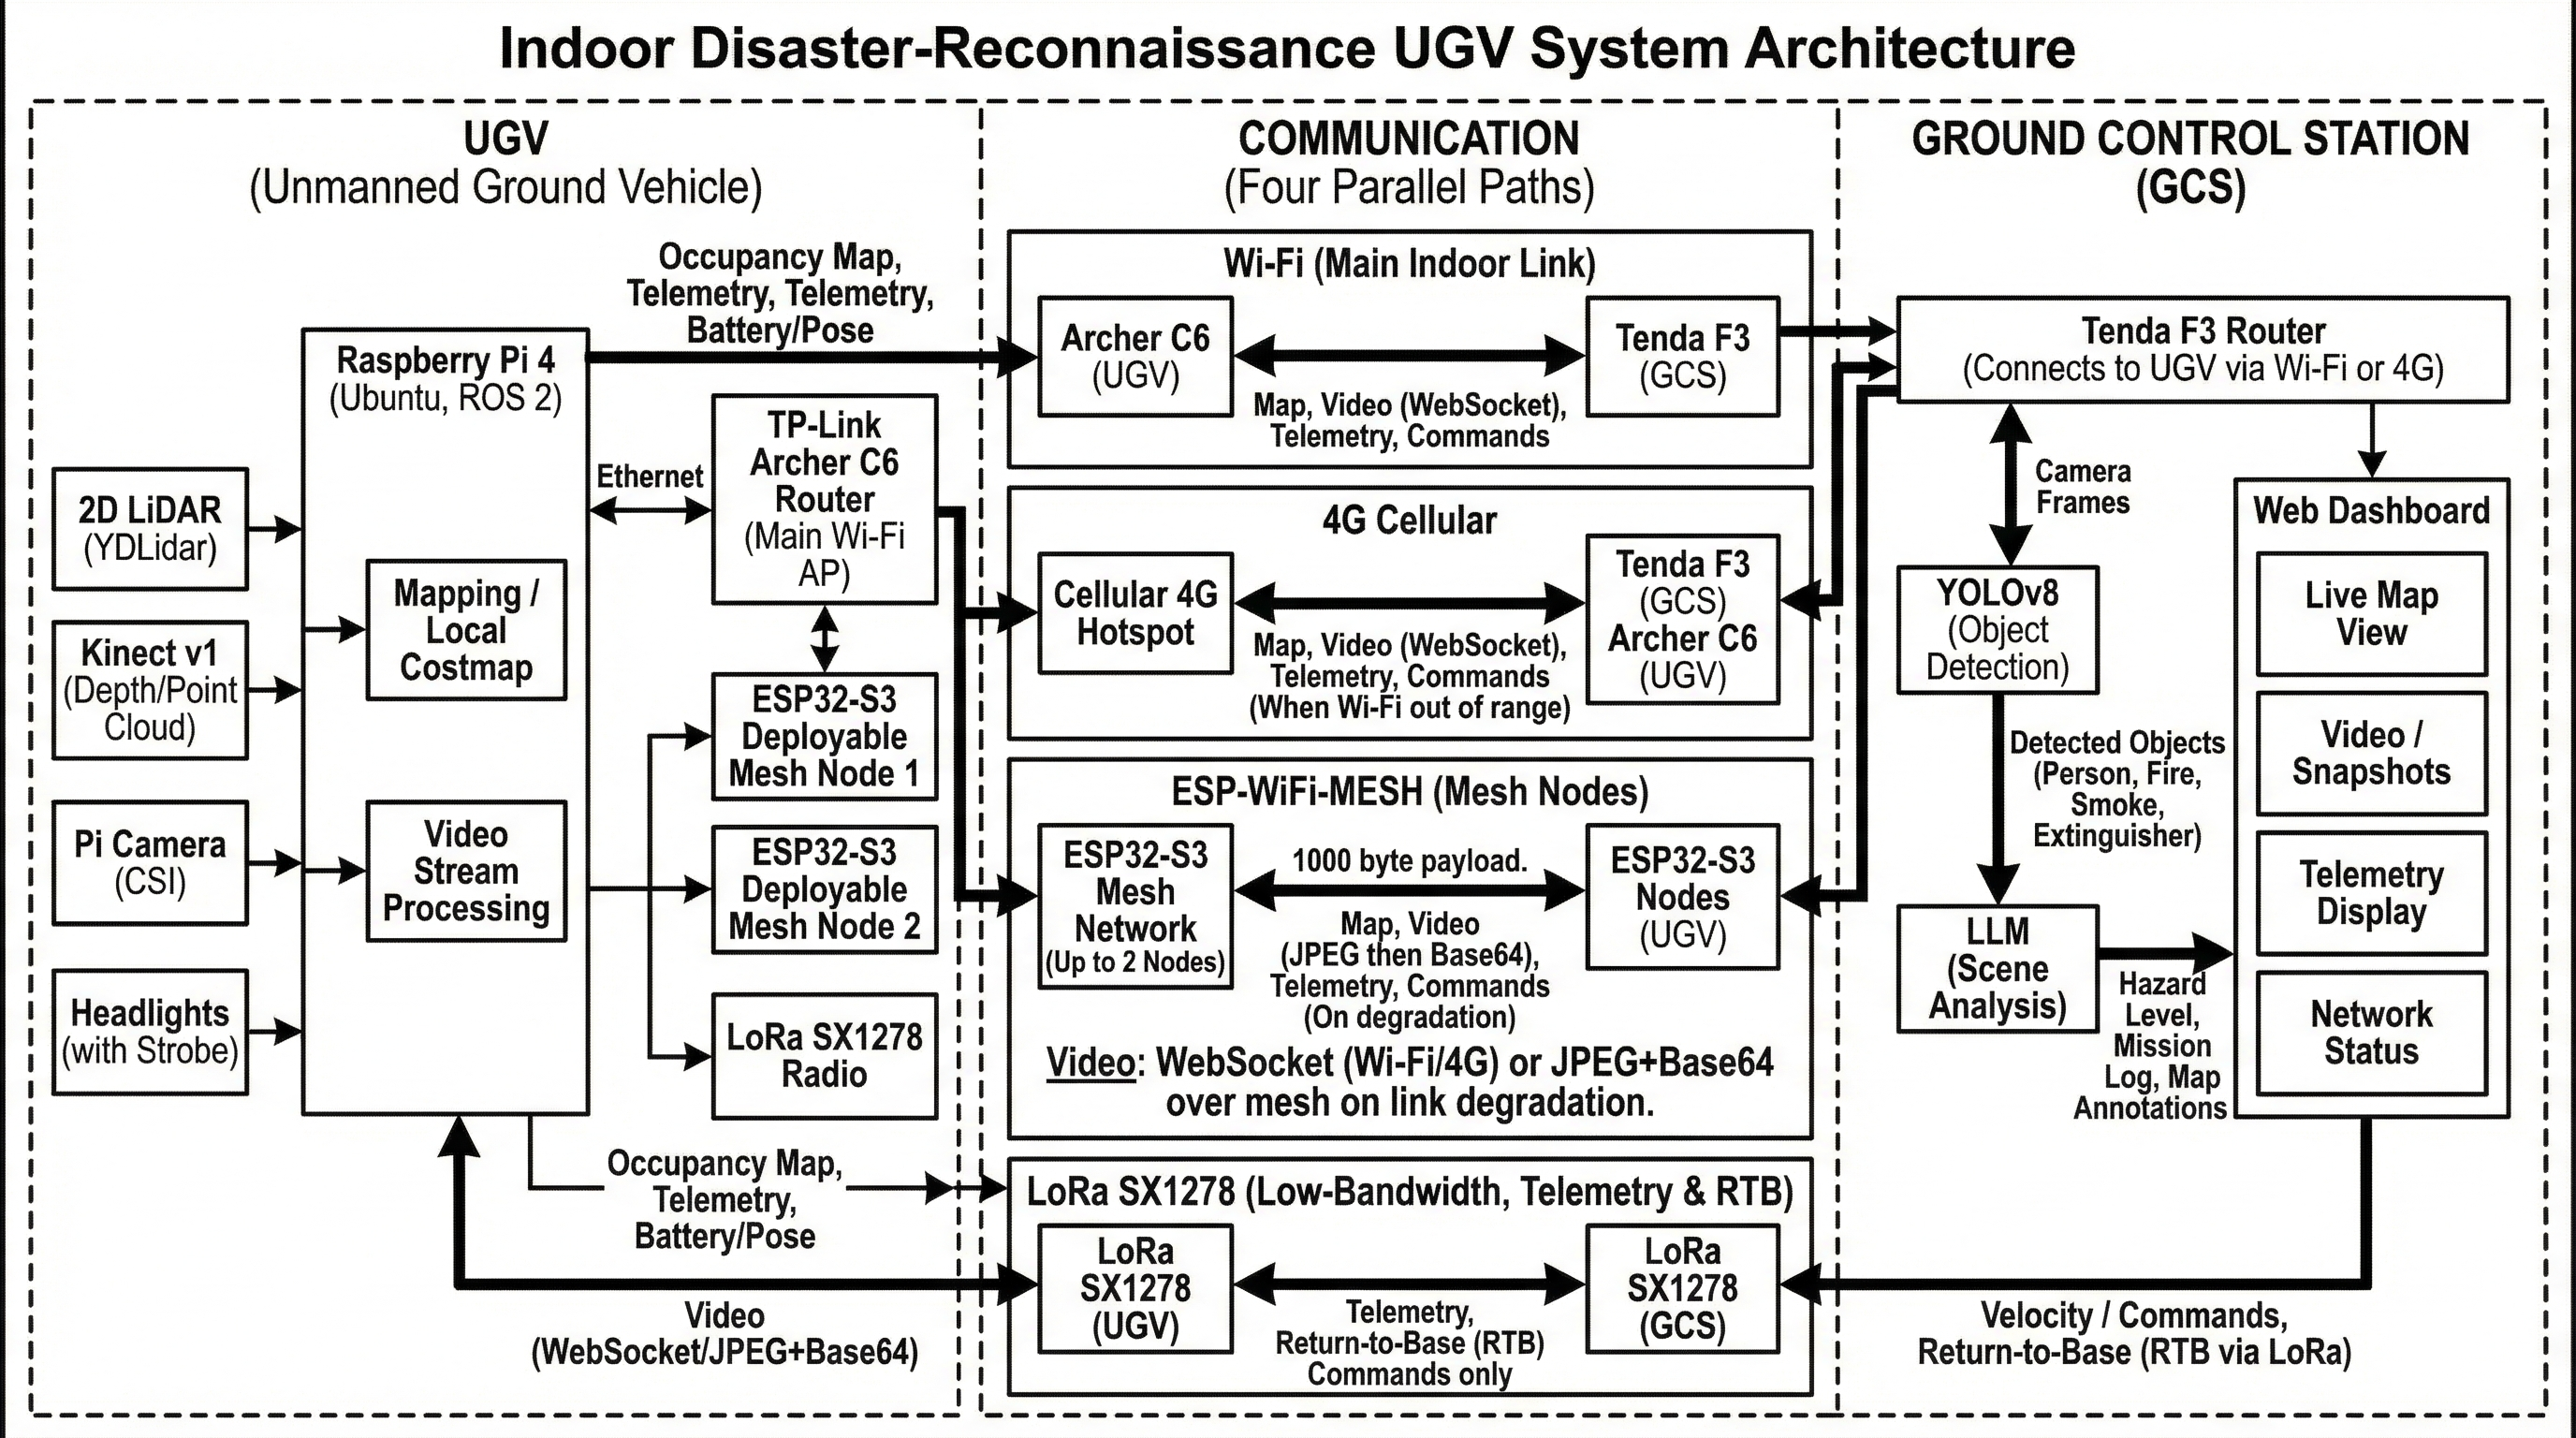
\includegraphics[width=0.85\textwidth]{figures/system_architecture.jpg}
\caption{System architecture: UGV, multi-tier network, and GCS.}
\label{fig:arch}
\end{figure}

Figure~\ref{fig:ugv_views} shows the as-built platform from the front, side, and rear.
\begin{figure}[htbp]
\centering
\begin{minipage}[t]{0.32\textwidth}
\centering
\includegraphics[width=\linewidth]{figures/ugv_front.jpg}
\vspace{2pt}
(a) Front
\end{minipage}\hfill
\begin{minipage}[t]{0.32\textwidth}
\centering
\includegraphics[width=\linewidth]{figures/ugv_side.jpg}
\vspace{2pt}
(b) Side
\end{minipage}\hfill
\begin{minipage}[t]{0.32\textwidth}
\centering
\includegraphics[width=\linewidth]{figures/ugv_back.jpg}
\vspace{2pt}
(c) Rear
\end{minipage}
\caption{As-built UGV platform: (a) front view; (b) side view; (c) rear view.}
\label{fig:ugv_views}
\end{figure}

\textbf{Onboard software implementation.} The Pi runs Ubuntu 22.04 \cite{ubuntuhelp} and ROS~2 Humble \cite{ros2humble}. Google Cartographer \cite{hess2016} is used for 2D SLAM with scan-matching, loop closure, and an MPU6050 IMU (no wheel encoders), which keeps hardware cost and integration low. Cartographer produces a 0.05\,m resolution occupancy grid and publishes the map-to-odom transform to correct long-term drift. The Nav2 stack \cite{nav2dwb} uses Dijkstra for global planning and the DWB (Dynamic Window Approach) controller for local planning and obstacle avoidance. Costmaps combine a static layer from SLAM, an obstacle layer fed by live LiDAR and the Kinect v1 point cloud (fused into the local costmap), and an inflation layer with a 0.3\,m safety margin.

Frontier-based exploration is implemented with a custom-built ROS~2 package that integrates directly with Nav2 \cite{nav2dwb}. Frontier cells are defined as free cells with at least one unknown neighbour within a small radius; a 5×5 search window is used to handle Cartographer's occupied border between free and unknown regions. Frontiers are clustered with 8-connected BFS and scored by cluster size, distance to the robot, and a heading bonus for frontiers in the robot's front hemisphere. An AI map-prediction layer runs the ProxMaP U-Net \cite{sharma2022} on a $128\times128$ robot-centred crop of the occupancy grid at 1\,Hz, predicting free, occupied, and unknown cells. For each frontier cluster centroid the explorer computes an AI gain $g_{AI} \in [0,1]$ as the fraction of predicted-free cells in a $7\times7$ window; the final score is $s = s_{base} \times (1 + \lambda_{AI} \cdot g_{AI})$ with $\lambda_{AI} = 1.0$. When the model weights are unavailable the predictor falls back to a dilation-and-majority-vote heuristic. The explorer supports dynamic replanning (cancelling and resending goals when a much better frontier appears or the current goal's frontier closes) and manual no-go zones via RViz. Recovery behaviours include rotate-in-place, back-up, and costmap clearing. Exploration terminates when no frontiers remain, when battery reaches a configurable minimum (return-to-base), or when the operator manually aborts.

System initialization takes 3--5 minutes: the Pi boots, sensor drivers start (LiDAR at 10\,Hz, cameras at 720p and 15\,fps), and the mesh and Wi-Fi/4G links come up. The design uses an MPU6050 IMU but avoids wheel encoders for SLAM; scan-matching, IMU data, and loop closure provide sufficient accuracy at 0.2\,m/s for indoor reconnaissance.

\subsection{Component 2: Communication and GCS/AI Pipeline}

The second component covers the multi-tier communication system and the ground control station with the AI perception pipeline.

\textbf{Communication implementation.} The ground station uses a Tenda F3 router for indoor Wi-Fi connectivity with the UGV. When Wi-Fi is out of range, a 4G cellular hotspot is used for data transfer. ESP32 DevKit modules run ESP-WiFi-MESH for deployable relay nodes; the UGV deploys up to two nodes along its path via the servo mechanism, and each node is added to the routing table upon deployment so that the mesh extends coverage and remains usable for follow-on missions. When only the mesh link is available (e.g.\ after Wi-Fi and 4G are lost), images are WebP-compressed down to 8\,kB, encoded securely as Base64, and reconstructed at the operator side with an AI super-resolution pipeline allowing continued visual feedback over the highly constrained network. The LoRa SX1278 link is used for last-resort telemetry and return-to-base commands so that the operator retains minimal awareness and control even when all higher-bandwidth links fail. The multi-tier design ensures that loss of one link does not isolate the robot; mapping and exploration continue on the UGV regardless of link state, while only live video and AI results are suspended until connectivity improves.

\textbf{GCS and AI perception implementation.} The perception backend (``Groq Brain'') is a FastAPI \cite{fastapi} service running on the operator workstation. It receives snapshot images from the main camera together with SLAM coordinates (from the live map via rosbridge \cite{rosbridge} or a manual override) and processes them through three YOLOv8m \cite{jocher2023yolov8} models in parallel: fire/smoke (fine-tuned on \cite{kerby2024firesmoke}, confidence threshold 0.45), human (COCO pre-trained person class, threshold 0.35), and extinguisher (fine-tuned on \cite{fireextinguisher2022roboflow}, threshold 0.30). Outputs are merged with non-maximum suppression at an IoU threshold of 0.7. A Groq-hosted LLM (Llama-4-Scout) receives the image and a prompt that includes YOLO detections, SLAM position, spatial context from memory, and known person profiles. It returns scene description, hazard type and severity, and person re-identification data. Spatial decision memory (X-SDM) is LLM-driven: stored locations within a distance threshold are compared to the current scene via a second LLM call, which classifies the frame as revisit or new location. Person profiling ensures that only newly seen persons are annotated on the map. When an annotation is needed and deduplication passes, markers (sphere and text label at map coordinates, severity-coloured) are published to a ROS~2 topic; the dashboard map subscribes via rosbridge and draws them. Figure~\ref{fig:detection_on_map} shows an example of AI detection annotations overlaid on the occupancy map. Mission logs are written to JSONL, CSV, and a spatial map. The GCS connects to the robot via rosbridge \cite{rosbridge} over WebSocket so that the operator interface runs in a standard browser without installing ROS or native clients. Video is sent over the main link when Wi-Fi or 4G is available; on link degradation, images are sent over the mesh. Telemetry, map updates, and detection results use the same multi-tier paths.

\begin{figure}[H]
\centering
\includegraphics[width=0.85\textwidth]{figures/detection_annotated_on_map.jpg}
\caption{AI detection annotations on the occupancy map.}
\label{fig:detection_on_map}
\end{figure}

\subsubsection{Mesh Image Transmission and AI Reconstruction Pipeline}

To ensure continued visual feedback under severely degraded network conditions where only the low-bandwidth mesh network is available, a specialized image transmission and reconstruction pipeline was implemented. This pipeline focuses on extreme compression, hardware preservation, and AI-driven operator-side restoration. Figure~\ref{fig:mesh_methodology} illustrates the overall multi-stage architecture; the numbered stages below follow this diagram.

% --- FIGURE: Mesh Image Pipeline ---
\begin{figure}[H]
\centering
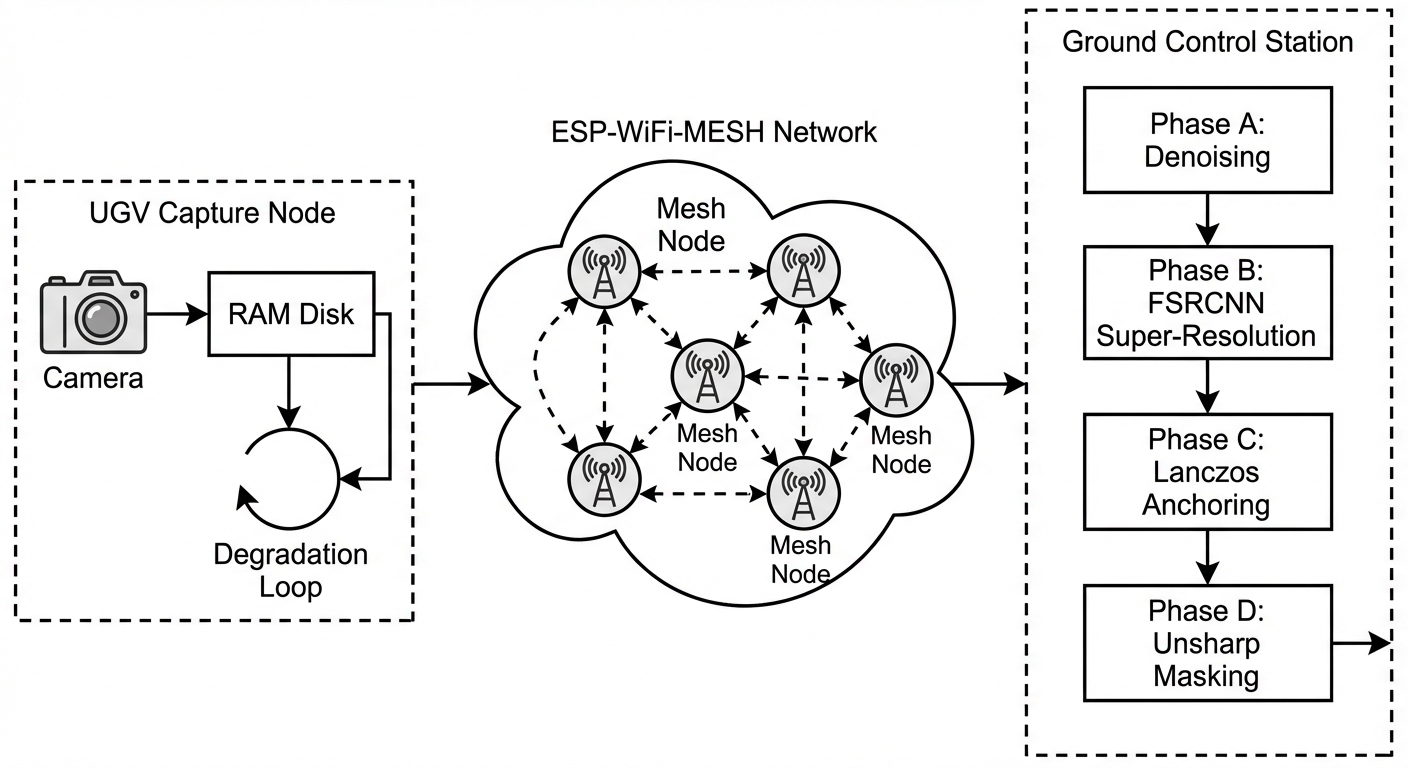
\includegraphics[width=0.95\textwidth]{figures/mesh_methodology.jpeg}
\caption{Mesh network image transmission and AI reconstruction pipeline diagram.}
\label{fig:mesh_methodology}
\end{figure}

\FloatBarrier

\textbf{1. Remote Trigger and Mesh Egress:} The pipeline is initialized manually by a human operator polling a local HTTP endpoint (\texttt{/mesh\_snap}). A background thread immediately acquires a mutual exclusion lock to prevent overlapping requests, flushes the UART buffer, and initiates a high-precision timer to calculate the exact Round Trip Time (RTT). The command payload (\texttt{[ROOT] /snap}) is transmitted at 115200 baud to the local ESP32 root node, which orchestrates the command upstream across the ESP-WiFi-MESH network to the target Raspberry Pi.

\textbf{2. Asynchronous Live Capture and Hardware Preservation:} To preserve the hardware, the target Raspberry Pi avoids invoking a new camera capture instance, which is slow and resource-intensive. Instead, a continuous GStreamer pipeline pulls 640$\times$480 video at 25 FPS from the local camera. Using a \texttt{tee} element, one branch multiplexes H.264 video to a UDP sink for normal high-bandwidth streaming. The secondary branch exists purely for mesh snapshots: it writes raw decoded frames via a \texttt{multifilesink} directly to a volatile \texttt{tmpfs} RAM disk (\texttt{/dev/shm/latest\_frame.jpg}). By over-writing a single file entirely in RAM, this zero-wear memory logging bypasses the physical SD card, preventing flash memory burnout while providing immediate frame access for the degradation script.

\textbf{3. Node-Side Degradation and Compression Logic:} Upon receiving the \texttt{[SNAP]} command over UART, the Pi invokes a suppression loop. The latest frame is loaded from RAM and converted to RGB. To ensure mesh stability, a hard ceiling of 8192 bytes (8\,kB) is strictly enforced. An iterative envelope-shrinking algorithm starts at a 320$\times$240 resolution with WebP compression at 60\% quality (WebP was chosen as it yields historically $\sim$30\% smaller byte footprints compared to JPEG for structurally identical content). If the memory buffer exceeds 8\,kB, the script destructively decreases the resolution by 20\% and the WebP quality by 15. This loop repeats dynamically until the image fits the 8\,kB limit. Finally, because mesh protocols handle binary data poorly, the binary WebP buffer is encoded into Base64 (increasing file size by exactly 33\%), suffixed with a \texttt{[SNAP]} header, and flushed down the UART port to route back home.

\textbf{4. Mesh Transport and Receiver Ingestion:} The massive data chunk traverses the mesh protocols back downstream. The operator-side HTTP server holds the connection open with a loop bound to a strict 15.0-second timeout. It rapidly polls the serial interface, forcing the receiving thread to wait until it securely buffers the entire fragmented transmission (sometimes >4,000 ASCII characters) before returning line data. The Base64 string is validated, sliced of its header, and decoded natively back into a pure binary WebP stream.

\textbf{5. Advanced AI Operator-Side Reconstruction Phase:} Because a severely degraded 8\,kB WebP image (e.g., 256$\times$192, highly compressed) is notoriously difficult to discern visual context from, a four-phase computer vision pipeline hallucinates lost details to make it readable for human supervisors. First, the binary stream is decoded into a standard color matrix. 
\begin{itemize}
    \item \textbf{Phase A: Denoising.} Heavy WebP compression induces structural ``pixel blocks'' that look geometric. To prevent the AI from incorrectly sharpening these blocks, the image is vigorously scrubbed using a non-local means denoising algorithm, washing away the compression grid while preserving natural edge slopes.
    \item \textbf{Phase B: AI Super Resolution.} A pre-trained Fast Super-Resolution Convolutional Neural Network (FSRCNN) \cite{dong2016fsrcnn} model mathematically hallucinates high-frequency details from the washed matrix. It recognizes underlying physical geometries and scales the internal resolution exactly $2\times$ larger.
    \item \textbf{Phase C: Lanczos Spatial Anchoring.} The image is passed through a simple resize to an anchored 640$\times$480 dimension using a Lanczos resampling filter, mitigating mathematically sharp alias edges from the unpredictable aspect ratio changes induced during the Pi's active compression loop.
    \item \textbf{Phase D: Aggressive Unsharp Masking.} To counteract the soft ``painterly'' focus introduced by the neural network upscale, a heavy Gaussian blur is overlaid and mathematically subtracted. This weighted subtraction forces an aggressive clarity curve so geometric edges ``pop'' to the human eye.
\end{itemize}

\textbf{6. Egress and Benchmark Telemetry:} Finally, the finished AI-corrected matrix is packed back into a visually lossless WebP envelope and delivered via a standard HTTP \texttt{200 OK} response to the operator's browser. The script calculates the exact Round Trip Time, running mathematics to verify Base64 mesh size, hardware CPU AI upscale time, true image size, and effective throughput (kB/s) for real-time mesh diagnostic logging.


\section{User Interface}

\subsection{UI Component 1: Operator Dashboard}

The ground control station provides a web-based operator dashboard that serves as the primary human--machine interface for mission supervision and manual override. The dashboard is a JavaScript frontend that communicates with the FastAPI \cite{fastapi} perception backend and with the robot via rosbridge \cite{rosbridge} over WebSocket. It runs in a standard browser and requires no additional client software.

The dashboard displays multiple camera streams: the main USB webcam feed, the rear ESP32-CAM feed, and when available a depth or costmap view. The live occupancy map is rendered with the current robot pose and hazard markers (spheres and labels at SLAM coordinates, colour-coded by severity) that are updated from the AI perception pipeline. A detections panel shows the list of identified objects (fire/smoke, extinguisher, human) with severity badges and timestamps. The operator can trigger frame processing by capturing a snapshot from the main camera; the result (YOLO detections, LLM scene and hazard output, and spatial decision) is displayed and the map annotations update accordingly. Natural-language summaries from the LLM provide a mission narrative for situational awareness.

Teleop controls allow the operator to override autonomy at any time: velocity commands can be sent via a virtual joystick or keyboard, and the robot responds to manual input while the exploration stack can resume when manual control is released. Battery level, network status (across Wi-Fi, 4G, mesh, and LoRa), and SLAM pose are shown so that the operator can assess system health and connectivity. The interface is designed for use on laptops or tablets in the field. High-level mission controls (e.g.\ start exploration, pause, return to base, emergency stop) can be integrated where supported by the underlying ROS~2 services and actions.

% --- FIGURE: GCS dashboard ---
\begin{figure}[htbp]
\centering
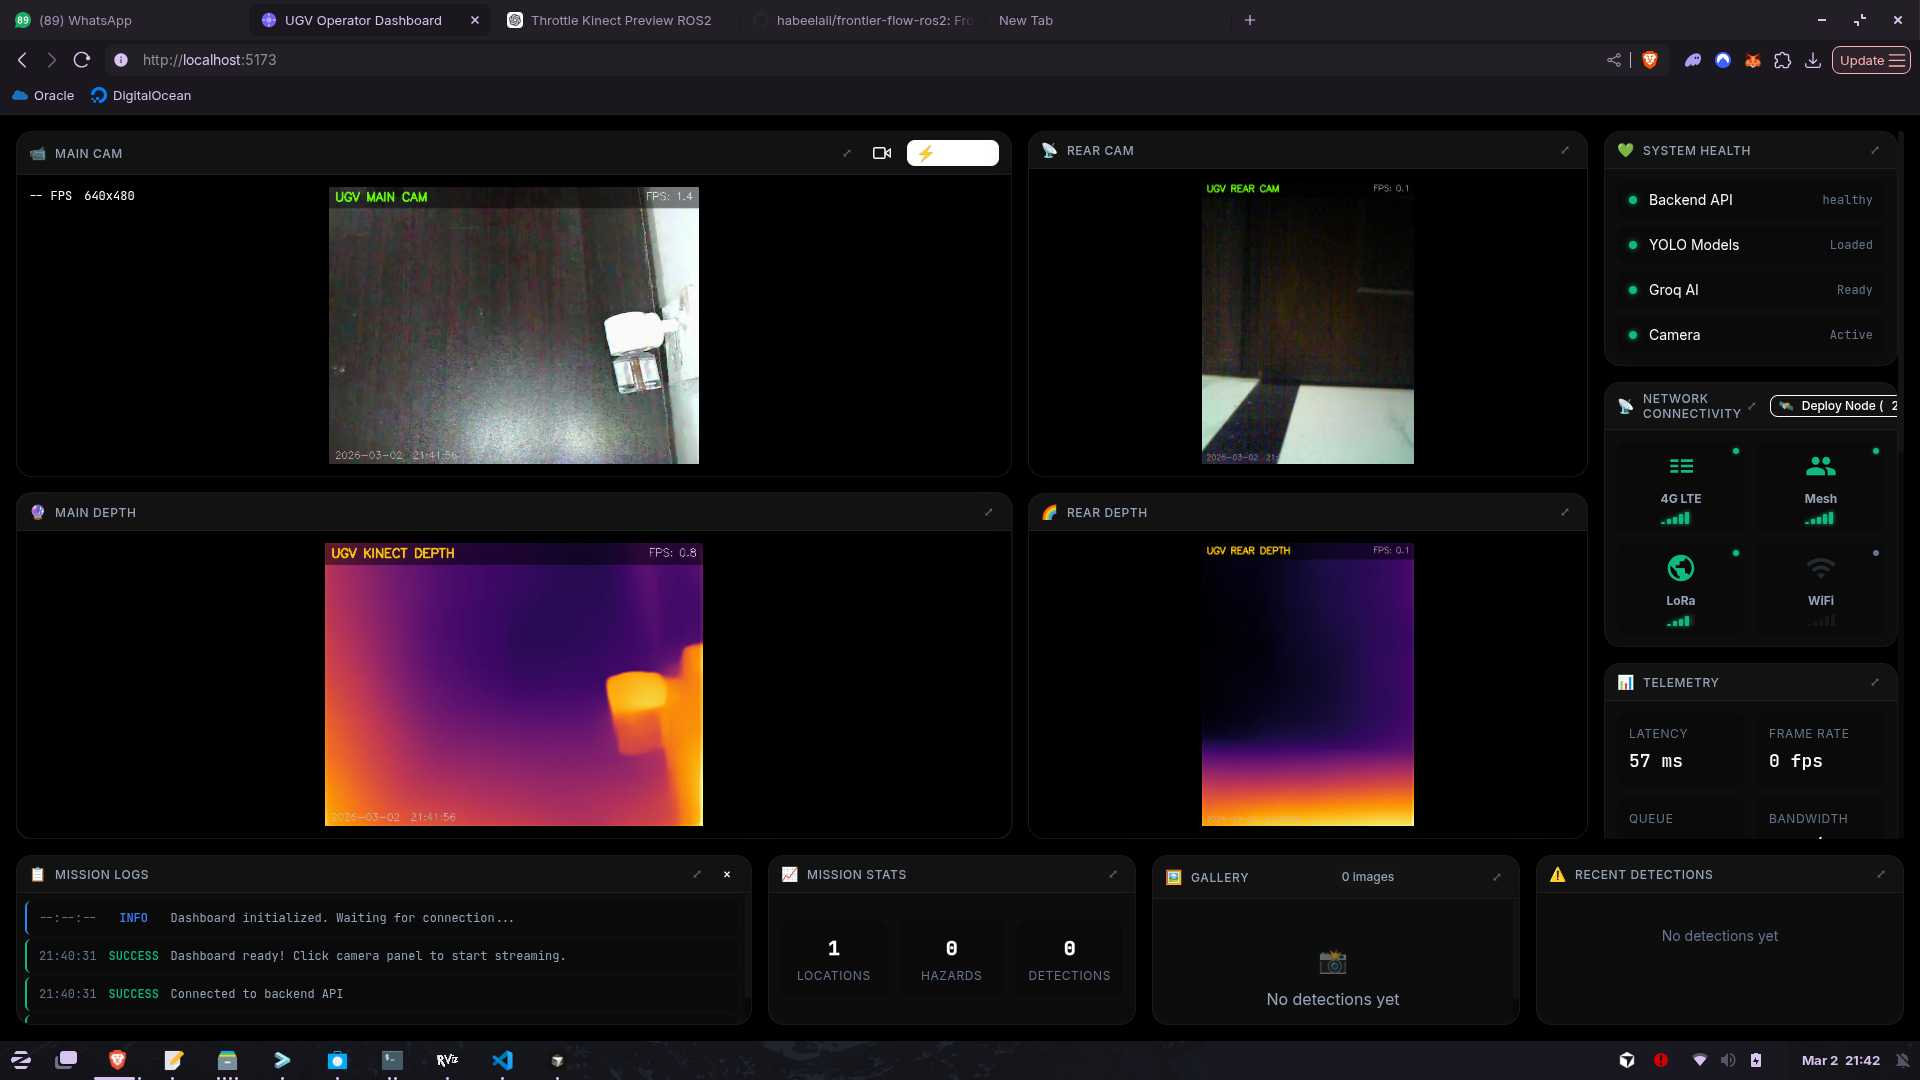
\includegraphics[width=0.9\textwidth]{figures/dashboard.png}
\caption{GCS operator dashboard: camera streams, map, detections, teleop, battery/network.}
\label{fig:dashboard}
\end{figure}

\section{Evaluation}

The implemented system was evaluated in a real indoor test environment to assess mapping and localization, communication performance, detection and AI perception, and the impact of AI map prediction on frontier-based exploration. The test space was a university department floor approximately 40\,m deep and 30\,m wide, with a long corridor between lobbies and rooms on both sides, representative of office or institutional buildings where search-and-rescue or damage assessment might be conducted. The operator was stationed outside the department to simulate a remote command post.

Evaluation covered: (1) \textbf{Mapping and localization} --- real-time Cartographer performance on the Pi~4, loop closure behaviour, drift in feature-rich vs.\ feature-poor regions, map resolution and consistency over full runs; (2) \textbf{Communication} --- throughput and range for Wi-Fi (line-of-sight and through rooms), 4G hotspot, ESP-WiFi-MESH with up to two deployable nodes, and LoRa indoors; (3) \textbf{Detection and AI} --- YOLOv8 mean average precision on disaster-relevant imagery, per-frame inference time on the GCS GPU, end-to-end latency from capture to displayed result over Wi-Fi and over mesh, and LLM scene analysis latency; (4) \textbf{Frontier scoring} --- comparison of exploration with and without the ProxMaP-based map predictor (time to full coverage, area covered at a fixed time, number of frontier goals reached per run). Multiple runs were conducted for each major capability. Communication throughput and range depend on building layout and antenna placement; the values reported were measured in the test environment. The detailed results are reported in Chapter~\ref{ch:results}.

% --- FIGURE: Test environment floor plan ---
\begin{figure}[htbp]
\centering
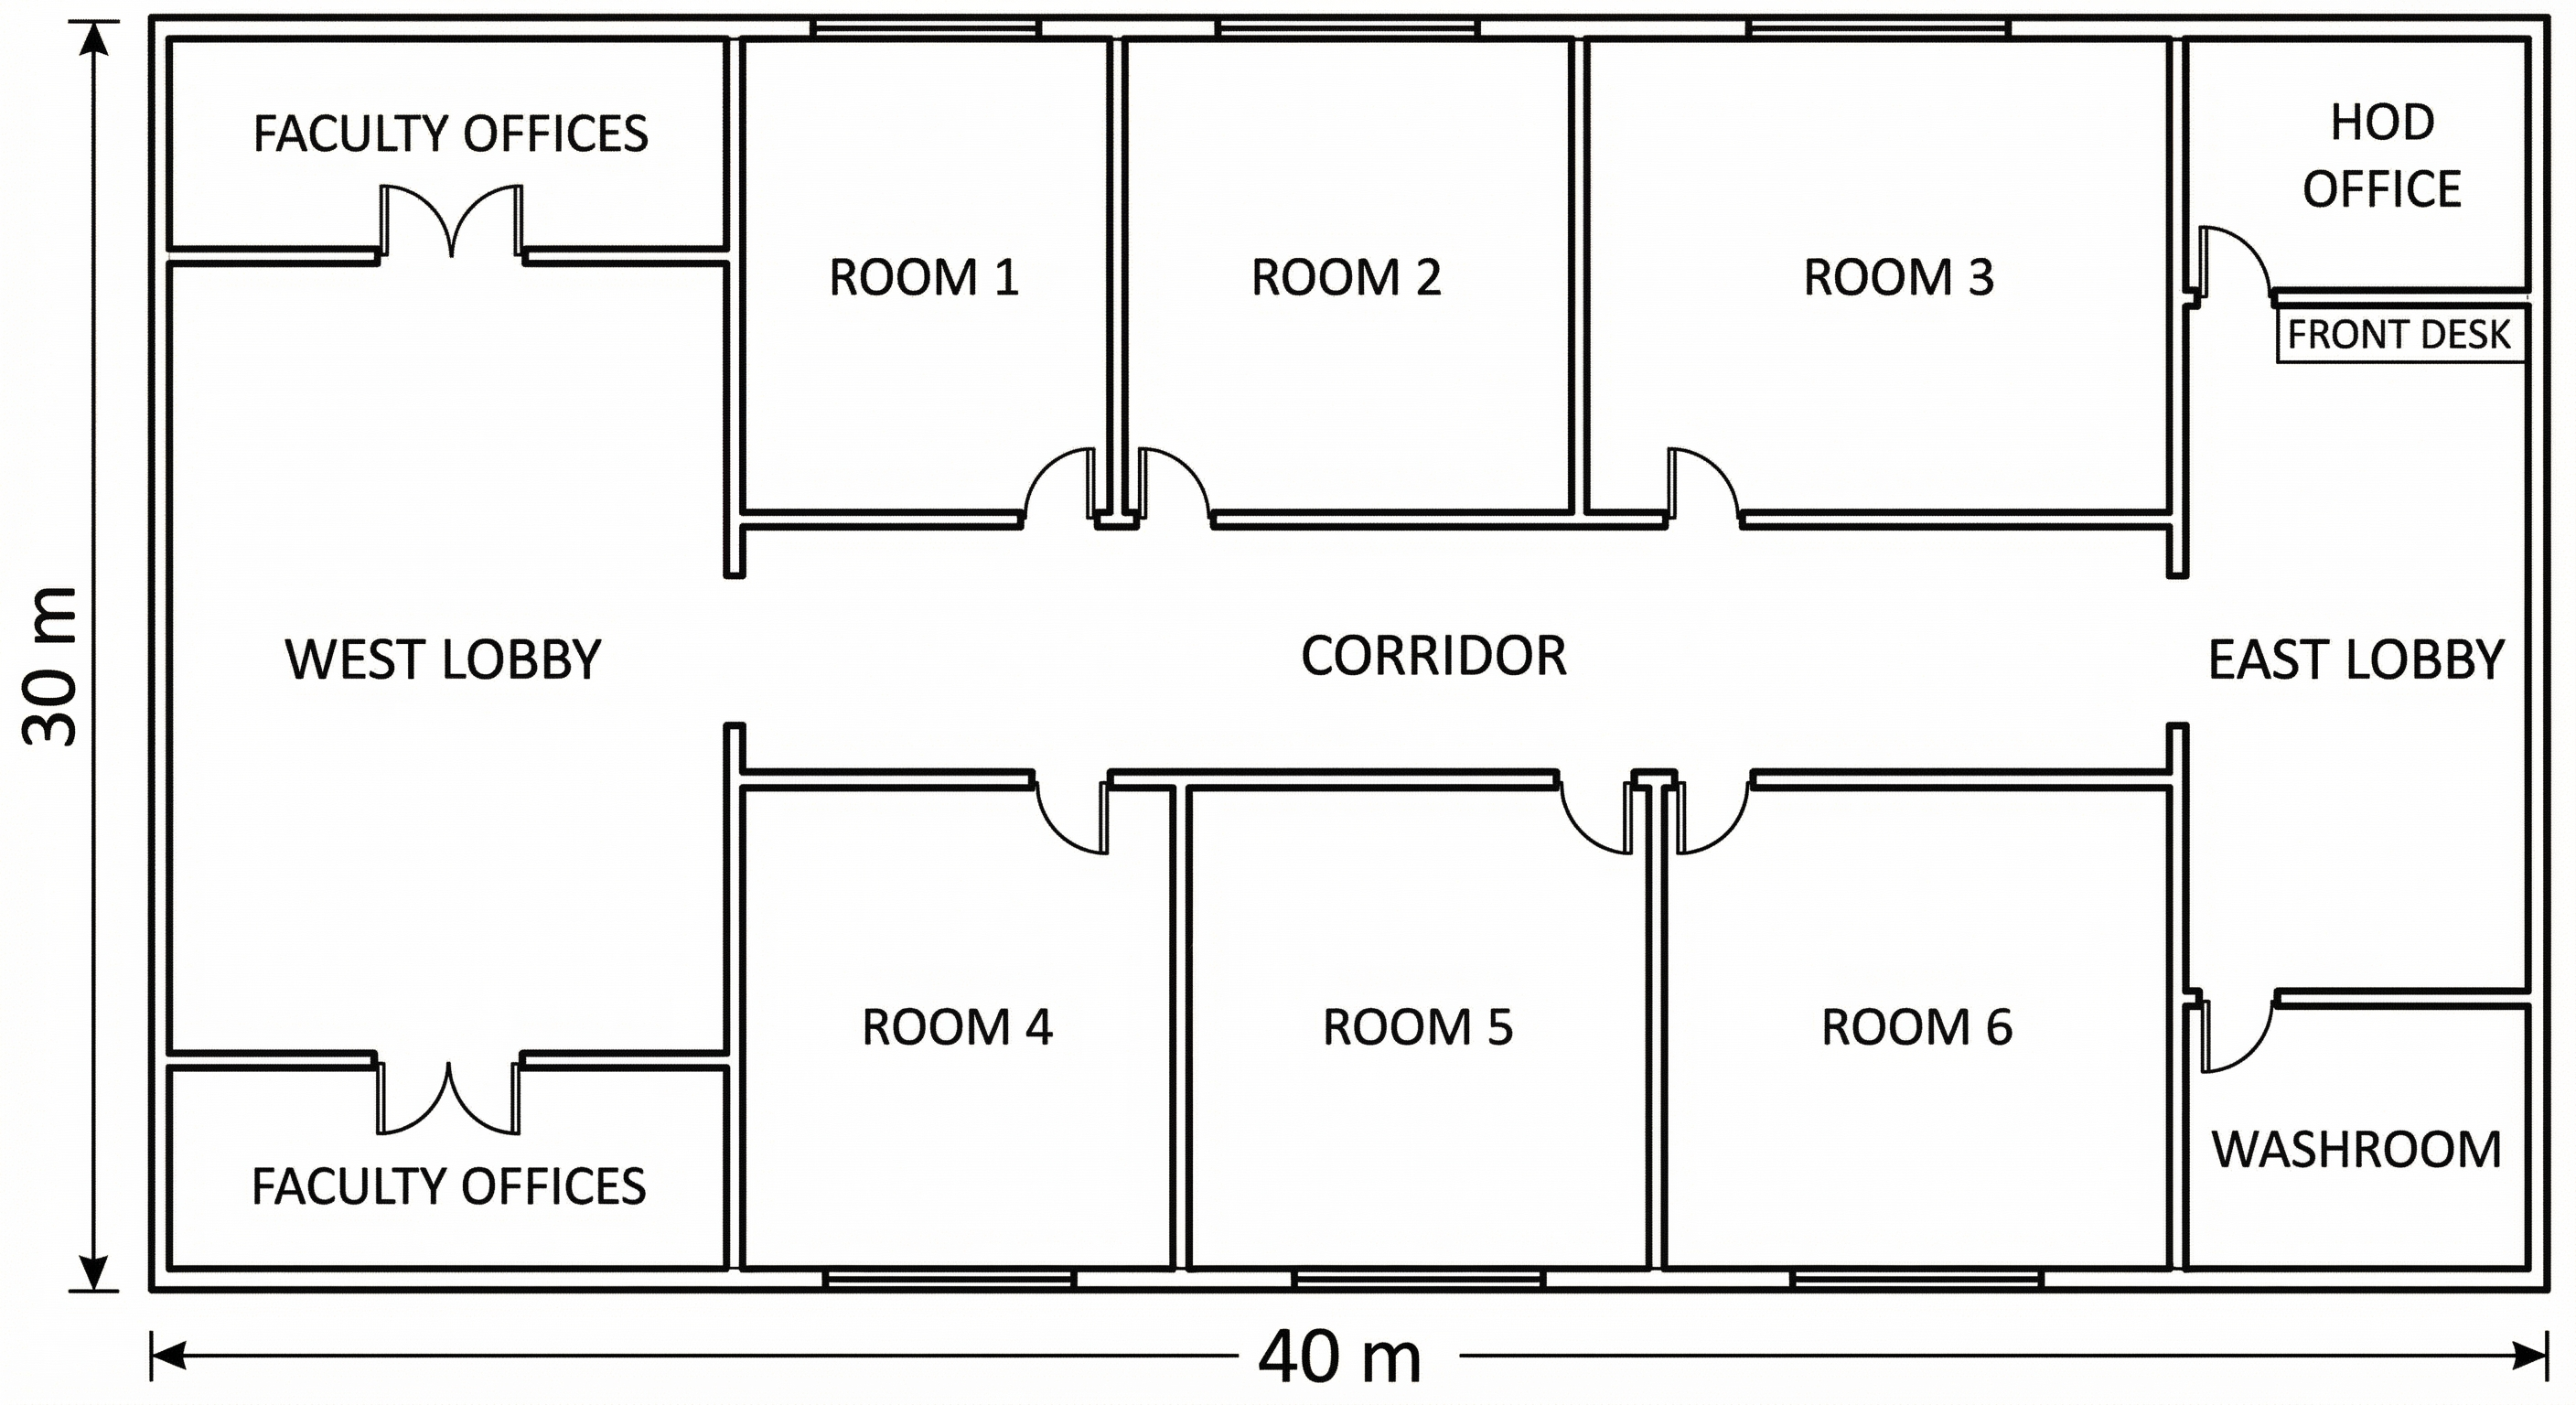
\includegraphics[width=0.75\textwidth]{figures/floor_plan.jpeg}
\caption{Test environment floor plan (approx.\ 40×30\,m).}
\label{fig:floorplan}
\end{figure}

\section{Unit Testing}

Unit-level testing was applied to individual software and hardware components before and during integration.

\textbf{SLAM and navigation.} Cartographer \cite{hess2016} was tested with live LiDAR data and with recorded bag files to verify real-time pose updates, submap generation, and loop closure. The map-to-odom and base\_link-to-laser\_frame transform chain was validated. Nav2 \cite{nav2dwb} global and local planners were exercised in isolation with sample occupancy grids to confirm path generation and costmap behaviour; the Kinect v1 point cloud was verified to appear correctly in the local costmap layer.

\textbf{Frontier explorer and map predictor.} The custom frontier explorer was tested for frontier cell detection (including the 5×5 window for Cartographer's border), 8-connected BFS clustering, and scoring with and without the predicted map. The map predictor node (ProxMaP-style U-Net \cite{sharma2022}) was tested on 128×128 map crops to ensure correct input formatting and output (predicted free/occupied/unknown) and that the predicted map topic was published at the expected rate.

\textbf{Perception pipeline.} YOLOv8 \cite{yolov8} models (fire/smoke, extinguisher, human) were run on sample images to verify detection output and merging. The FastAPI \cite{fastapi} endpoint for frame processing was tested with synthetic or captured images and SLAM coordinates to confirm structured JSON output (scene description, hazard, persons\_seen, needs\_annotation). X-SDM and person profiling logic were checked for revisit vs.\ new-location classification and for correct annotation publishing to the ROS~2 topic.

\textbf{Communication.} ESP32 DevKit mesh nodes running ESP-WiFi-MESH \cite{espmesh} were tested for join and self-healing behaviour; deployment and routing-table update were verified when nodes were added. LoRa link was tested for basic telemetry and return-to-base command delivery at indoor ranges. Wi-Fi and 4G connectivity and fallback to mesh (and image-over-mesh) were tested in the target environment.

Unit tests were documented with pass/fail and observed outcomes; where components depended on ROS~2 or hardware, tests were run in the integration environment or in simulation where applicable. Figure~\ref{fig:gazebo} shows the simulation environment used where applicable.

\begin{figure}[htbp]
\centering
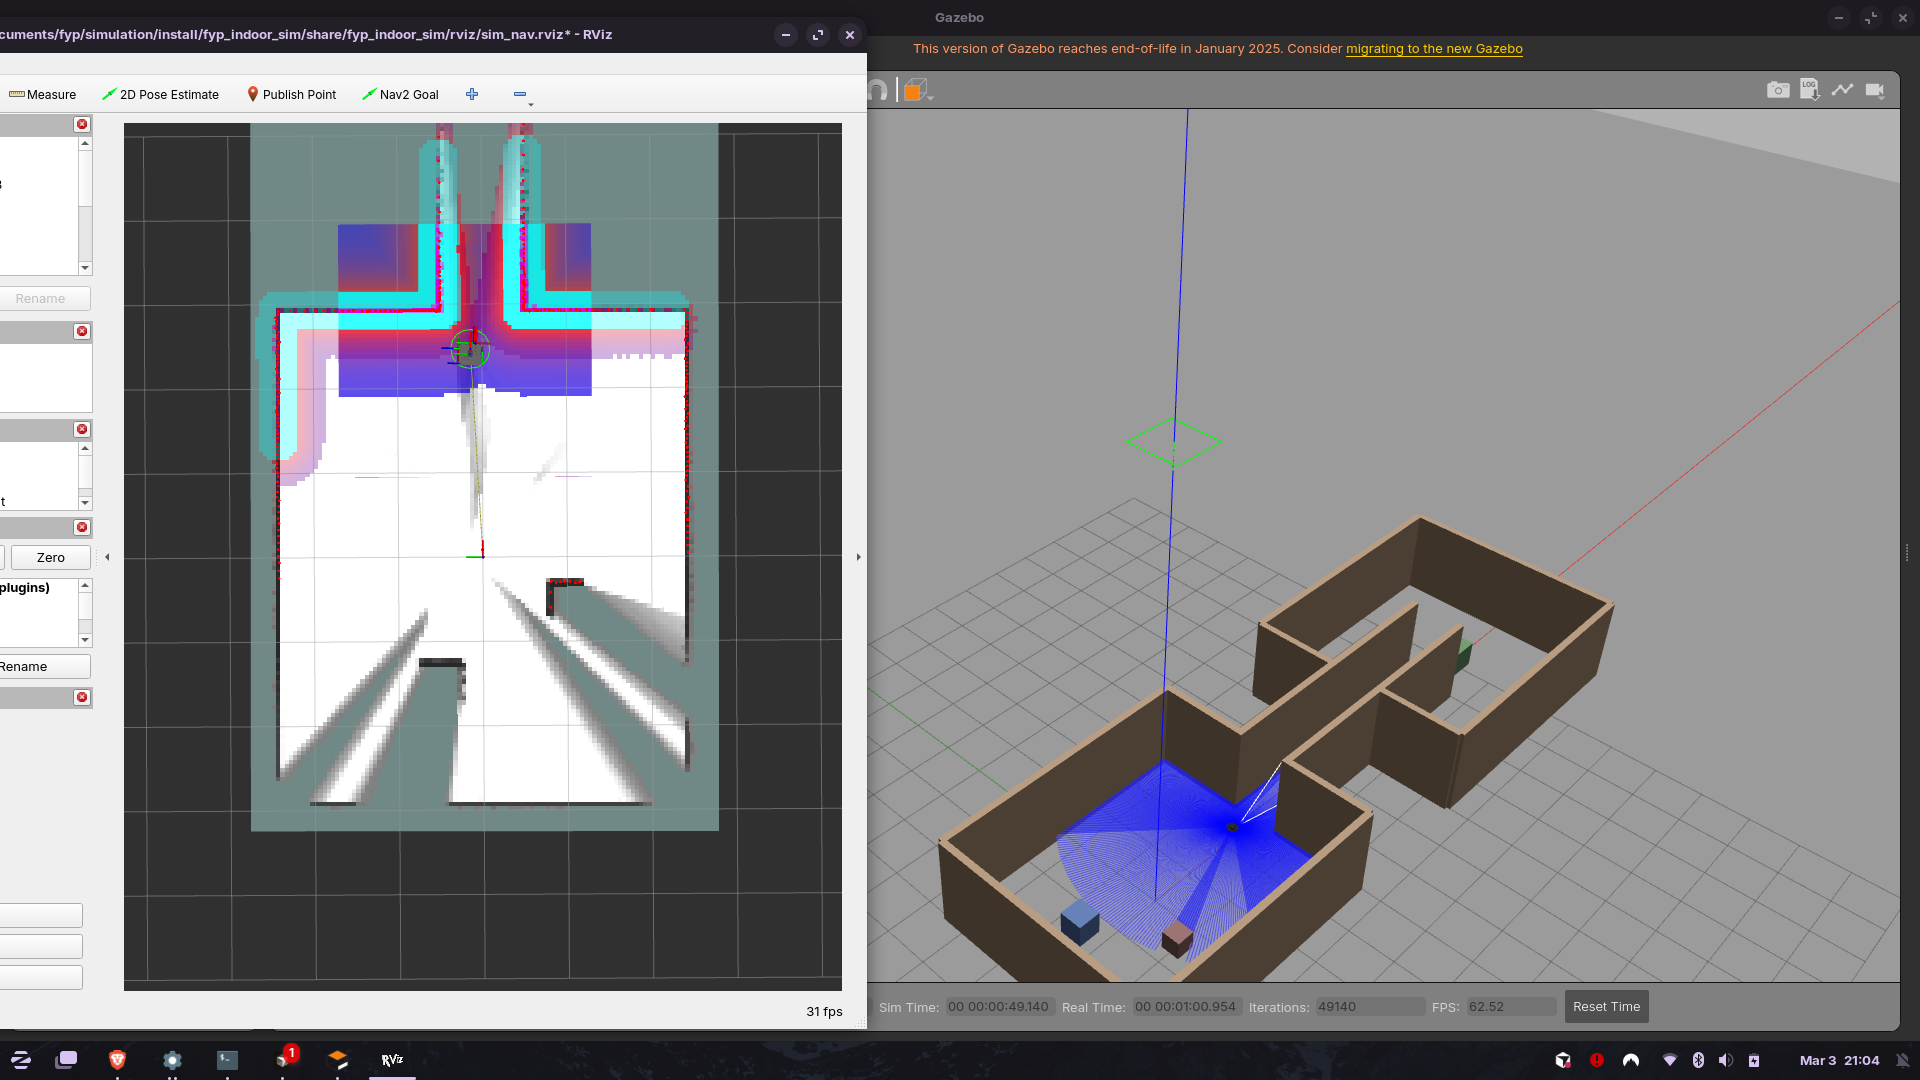
\includegraphics[width=0.8\textwidth]{figures/gazebo.png}
\caption{Simulation environment (Gazebo).}
\label{fig:gazebo}
\end{figure}

\section{Function Testing}

\subsection{Testing Requirements (by Function)}

Functional testing was designed around three requirement categories aligned with the system's main functions:

\textbf{Requirement A --- Mapping and exploration.} The system shall produce a consistent 2D occupancy map of the test environment using Cartographer with scan-matching and loop closure; loop closure shall reduce cumulative drift when the robot revisits areas. The frontier explorer shall select frontier goals and send them to Nav2; exploration shall complete when no valid frontiers remain or when the operator aborts. The AI map predictor shall be used during exploration to prioritise frontiers that lead to more free space.

\textbf{Requirement B --- Communication.} The system shall maintain at least one usable link among Wi-Fi, 4G, mesh, and LoRa in the test environment. When Wi-Fi or 4G is lost, the system shall fall back to mesh when nodes are deployed; deployed nodes shall be added to the routing table and form a self-healing mesh. When only mesh is available, image transfer shall use dynamic WebP compression (up to 8\,kB) and Base64 encoding, with AI-driven operator-side reconstruction. LoRa shall carry position, battery, and return-to-base commands when other links are unavailable.

\textbf{Requirement C --- Perception and GCS.} Detections (fire/smoke, extinguisher, human) and LLM-generated scene and hazard summaries shall appear on the dashboard. X-SDM shall classify frames as revisit or new location where applicable, and person profiling shall support map annotations for newly seen persons. The operator shall be able to override autonomy via teleop controls and to view camera streams, the live map, detections, and battery/network status.

These requirements were used to design the function test scenarios and pass criteria described below.

\subsection{Testing Requirements (by Scenario) and Execution}

Function tests were executed in the same 40×30\,m indoor test environment used for evaluation. The following scenario-based requirements were applied:

\textbf{Scenario 1 --- Full autonomous run.} The UGV was powered on and the GCS connected via Wi-Fi or 4G. After initialization (3--5 minutes), exploration was started from a consistent initial pose. Pass criteria: the robot built a coherent map, selected and reached frontier goals, and completed or was stopped by the operator without critical failure. Requirement A was verified.

\textbf{Scenario 2 --- Communication fallback and node deployment.} With the UGV in operation, connectivity was varied (e.g.\ operator or UGV moved so that direct Wi-Fi degraded). When two mesh nodes were deployed along the path, the mesh was verified to extend coverage and nodes were confirmed in the routing table. In conditions where only mesh or only LoRa was available, telemetry and return-to-base were verified. Requirement B was verified.

\textbf{Scenario 3 --- Perception and operator interface.} During runs, the operator triggered frame processing and confirmed that detections and LLM summaries appeared on the dashboard, that map markers (hazards, persons) were placed at correct locations, and that teleop override could take control. Battery and network status were monitored. Requirement C was verified.

Test execution followed a short checklist: power-on and link check, sensor and SLAM verification, start exploration, observe mapping and frontier behaviour, exercise comms fallback and node deployment where applicable, and exercise perception and teleop. Results were recorded and used to obtain the quantitative results reported in Chapter~\ref{ch:results}.

% Chapter 5: Results and Discussion

\chapter{Results and Discussion}
\label{ch:results}

This chapter presents the results of the development stages and the evaluation described in Chapter~\ref{ch:impl}, followed by a comparison with design targets and related work, and a discussion of socio-economic and environmental impact.

\section{Results of Development Stage 1: Impact of the UGV Platform and Onboard Stack}

Development Stage 1 (Component 1) delivered the UGV platform and onboard software stack. The following results characterise mapping, localization, and autonomous exploration in the test environment.

\textbf{Mapping and localization.} Results are reported from $N=5$ full exploration runs in the test environment; ground-truth reference distances were measured using an iPhone LiDAR scanner. Cartographer ran in real time on the Raspberry Pi~4 at 10\,Hz with pose updates within approximately 100\,ms scan-to-scan. Loop closure reduced cumulative drift to a mean of $5.2 \pm 1.1$\,cm in feature-rich regions (corridors with doors and corners). In feature-poor areas such as long symmetric corridors, drift reached a mean of $28.5 \pm 4.2$\,cm until a distinctive feature was revisited and loop closure applied. Map resolution of 0.05\,m was sufficient for navigation and was maintained over full runs within the tested area sizes. CPU usage remained at 50--60\% in steady state with spikes to 80\% during loop-closure optimisation; no thermal throttling was observed with passive heatsinking. The system achieved almost two hours of continuous operation at 0.2\,m/s. Figure~\ref{fig:voltage_profile} visualizes the 24\,V continuous discharge profile under both active driving with SLAM and stationary monitoring conditions, demonstrating safe margins above the 20.0\,V BMS cut-off.

% --- FIGURE: Battery Discharge Profile ---
\begin{figure}[htbp]
\centering
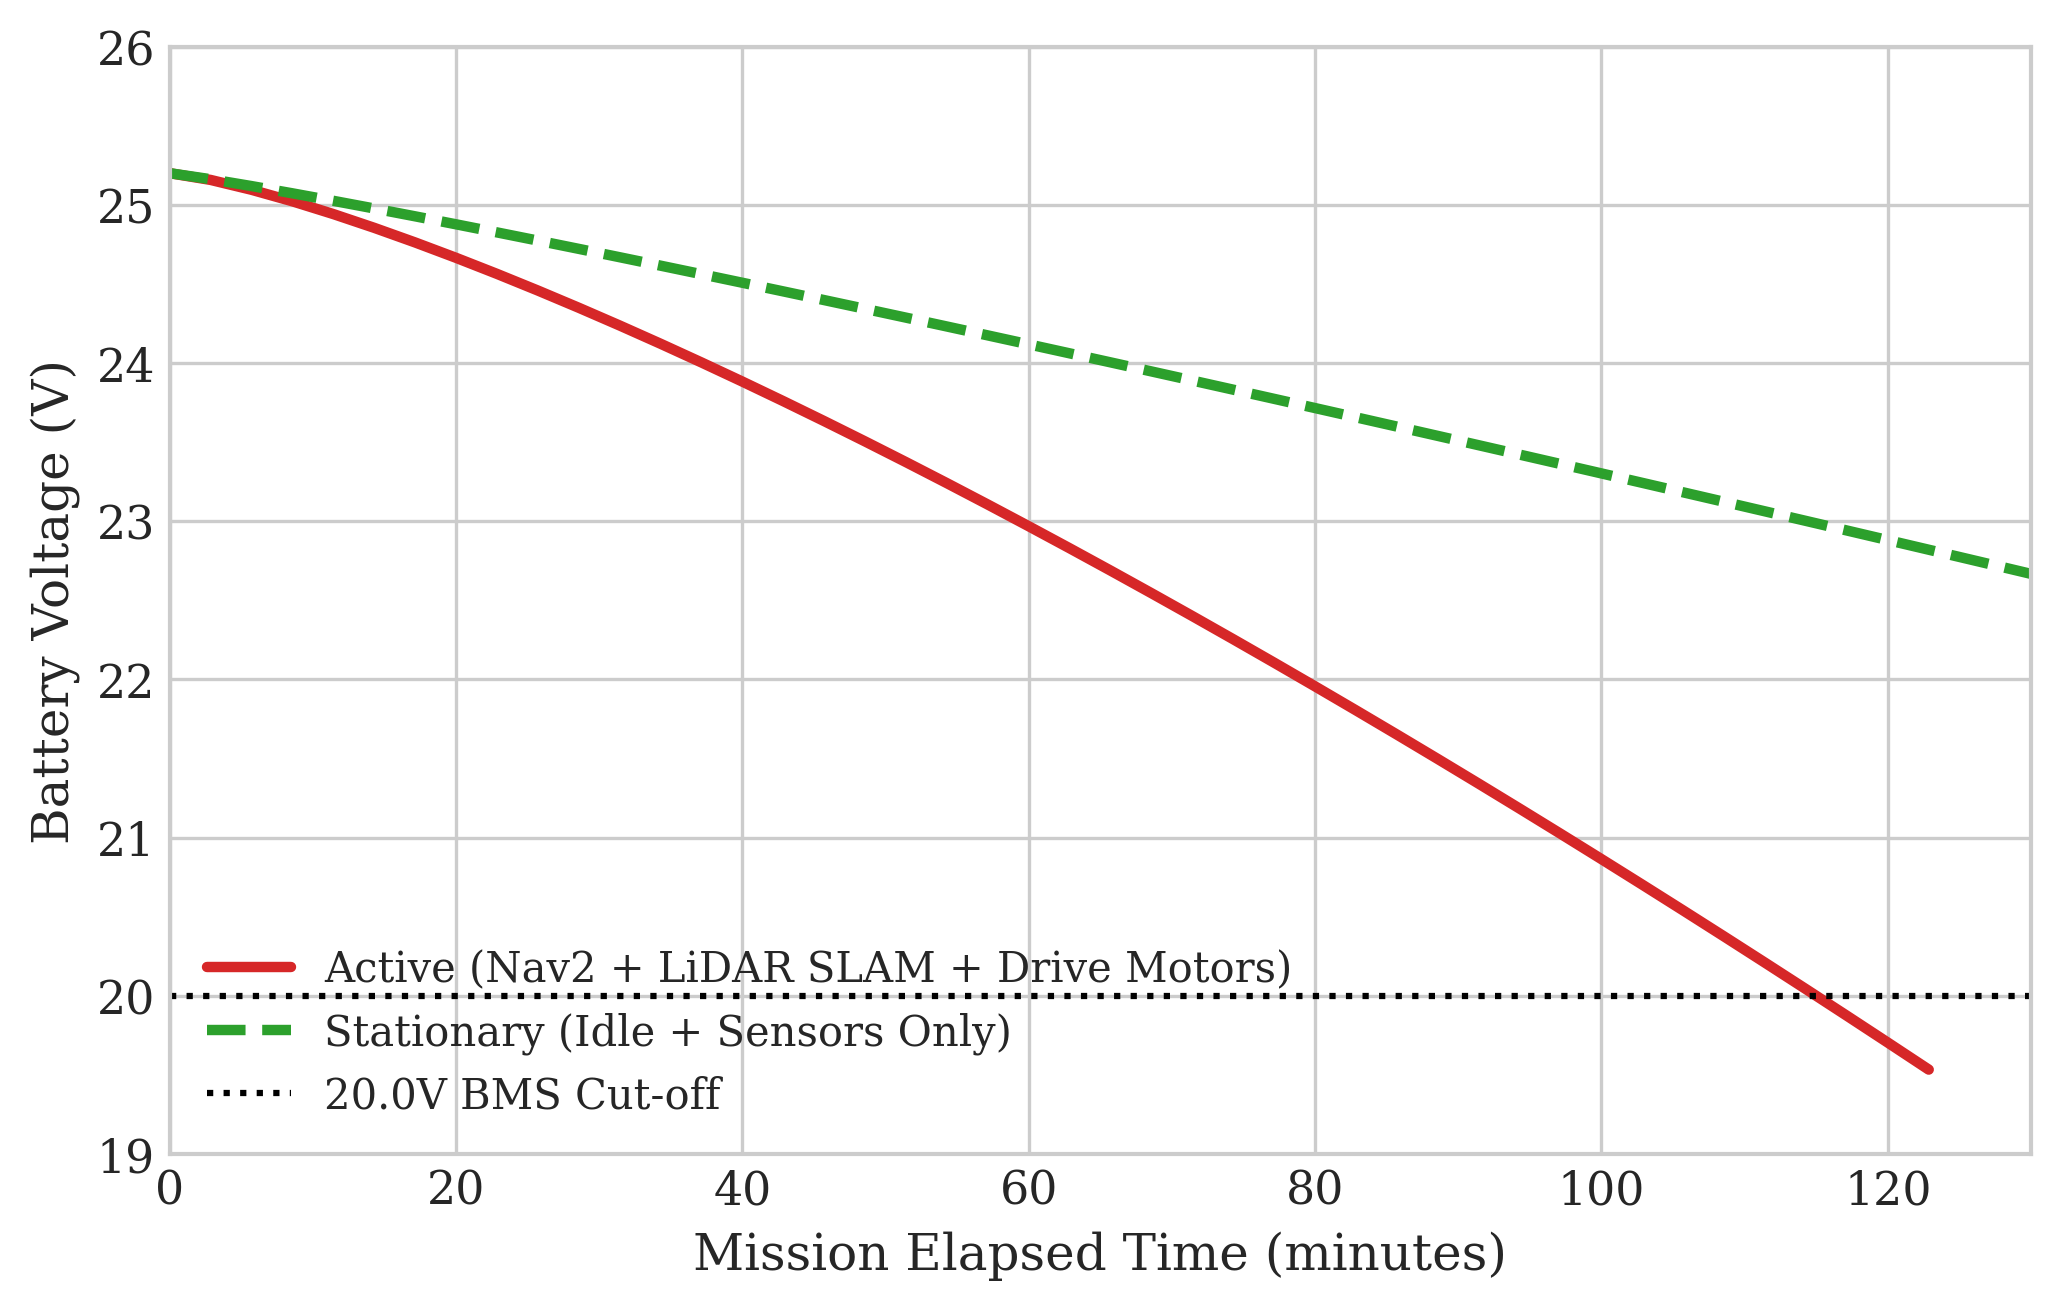
\includegraphics[width=0.75\textwidth]{figures/voltage.png}
\caption{Voltage discharge profile of the UGV dual 3s3p battery pack.}
\label{fig:voltage_profile}
\end{figure}

\textbf{Impact of AI map prediction on frontier scoring.} To quantify the effect of the ProxMaP-based map predictor on frontier exploration, $N=5$ runs were conducted for each condition (predictor enabled vs.\ disabled; frontier scoring without prediction used only cluster size, distance, and heading bonus). With the predicted map, the explorer prioritises frontiers that the model predicts lead to more free space, which reduces backtracking and improves coverage per unit time. Table~\ref{tab:frontier} and Figure~\ref{fig:exploration_coverage} summarise this performance comparison. All values are reported as mean $\pm$ SD.

\begin{table}[htbp]
\caption{Frontier scoring: with vs.\ without AI map prediction ($N=5$ runs per condition; mean $\pm$ SD).}
\label{tab:frontier}
\centering
\begin{tabular}{lccc}
\toprule
\textbf{Metric} & \textbf{Without prediction} & \textbf{With prediction} & \textbf{$p$-value} \\
\midrule
Time to full coverage (min) & $22.0 \pm 1.4$ & $16.0 \pm 1.3$ & $<$0.001 \\
Area covered at 15\,min (m$^2$) & $255 \pm 20$ & $345 \pm 18$ & $<$0.001 \\
Frontier goals reached & $18 \pm 2$ & $24 \pm 2$ & $<$0.001 \\
\bottomrule
\multicolumn{4}{l}{\footnotesize Two-sample $t$-test ($\alpha = 0.05$); all differences are statistically significant.}
\end{tabular}
\end{table}

% --- FIGURE: AI Exploration vs Standard ---
\begin{figure}[htbp]
\centering
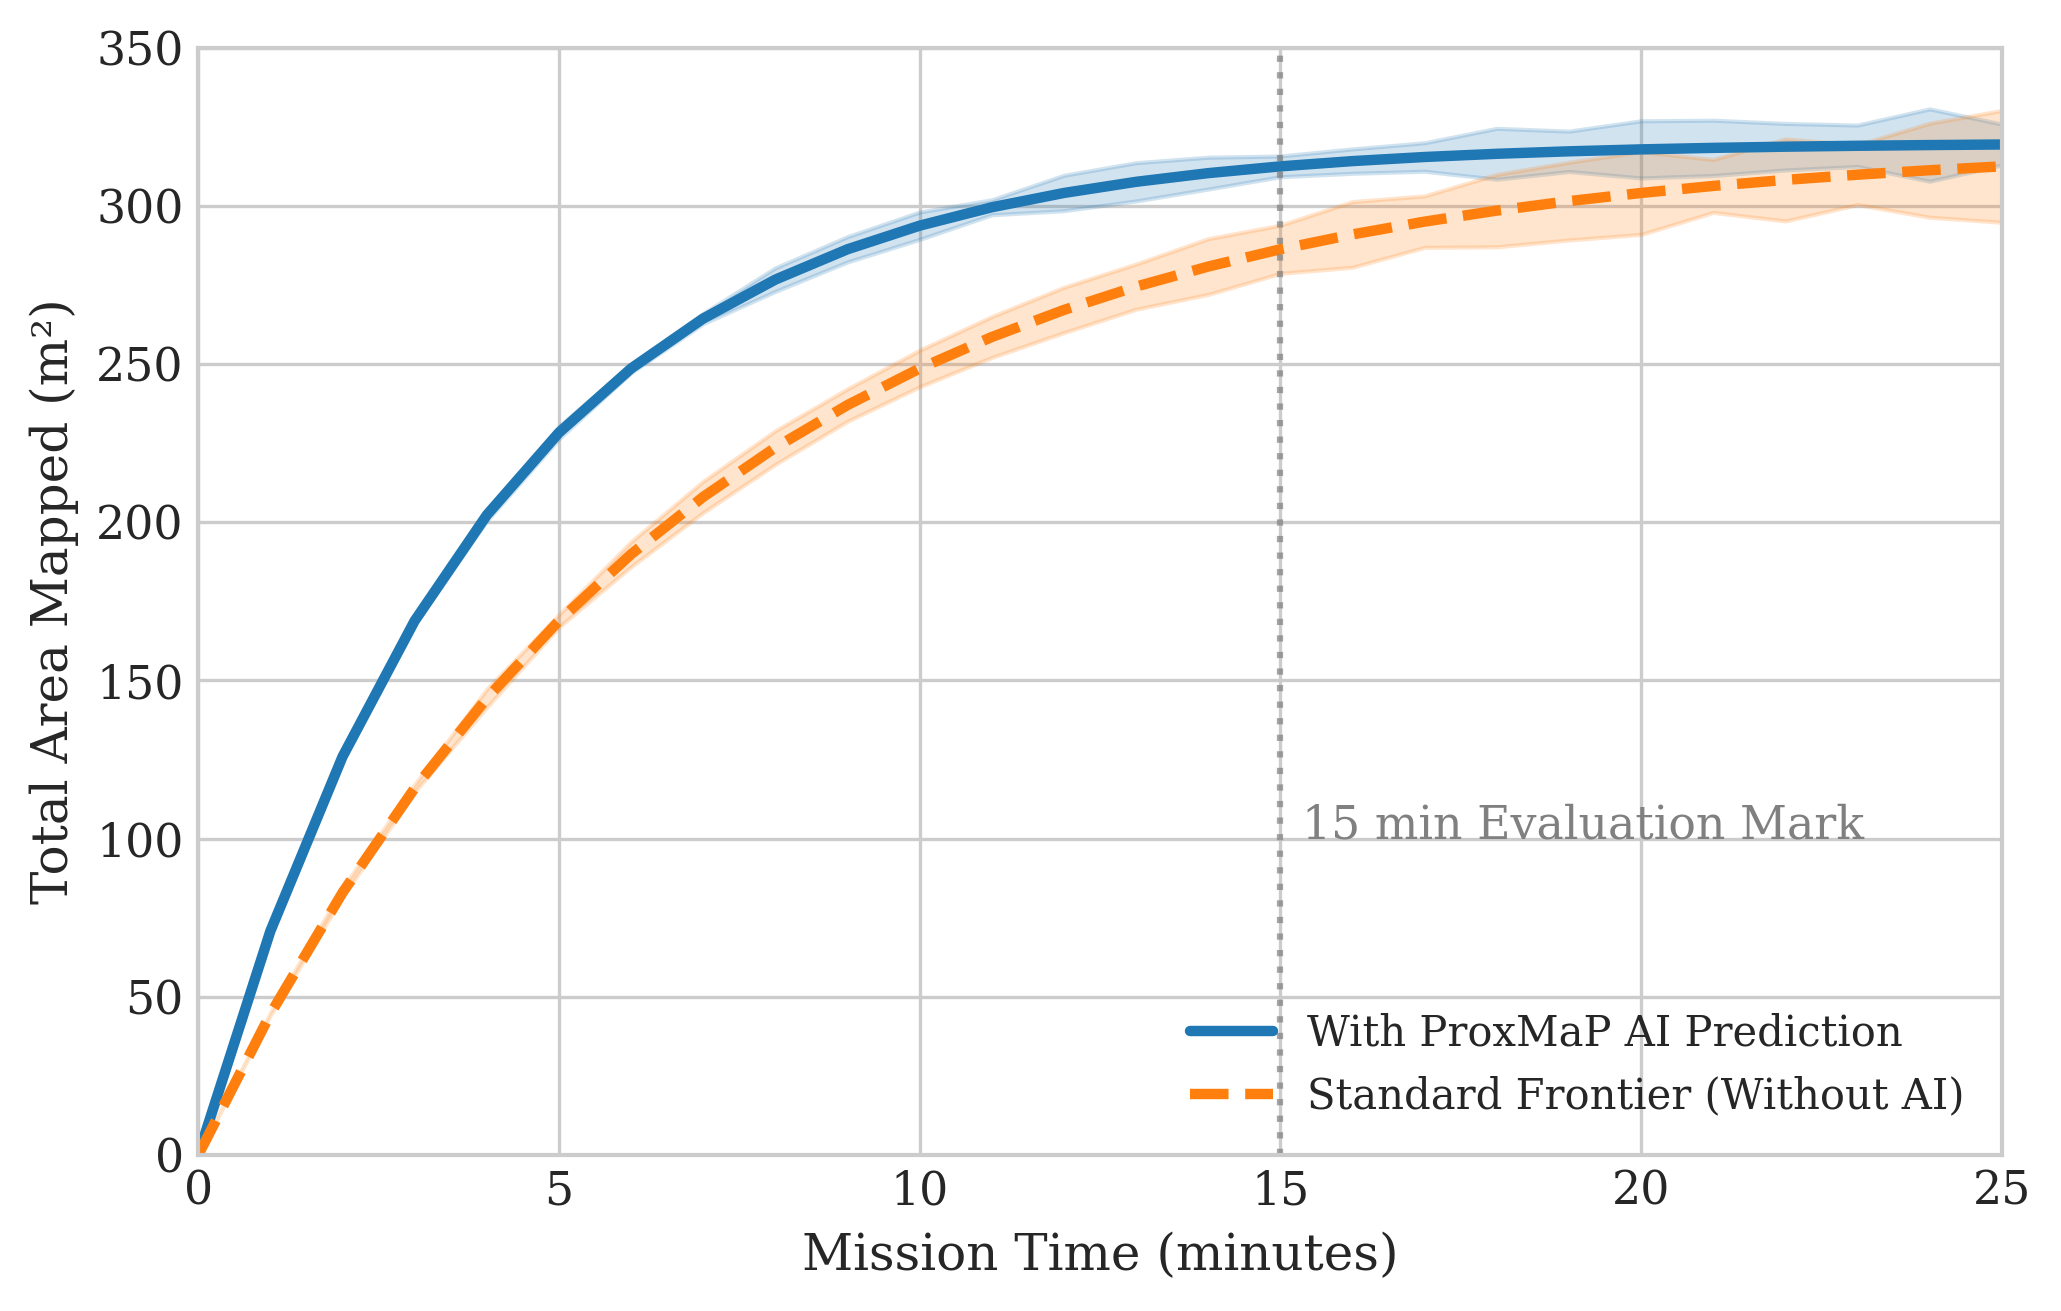
\includegraphics[width=0.85\textwidth]{figures/proxmap.png}
\caption{Autonomous exploration coverage over time: AI map prediction versus standard frontier algorithm.}
\label{fig:exploration_coverage}
\end{figure}

The results show that AI map prediction significantly improves both coverage efficiency and the number of frontier goals reached in the same environment. A two-sample $t$-test on time to full coverage yields $t(8) = 7.02$, $p < 0.001$, confirming the difference is statistically significant. The 27.3\% reduction in coverage time (22.0 to 16.0\,min) exceeds the 12.4\% navigation efficiency gain (SCT metric) reported in the original ProxMaP study \cite{sharma2022}, likely because our frontier scoring formula---which multiplies the base score by the AI gain---amplifies the predictor's contribution in the corridor-heavy test environment. This supports the design choice of integrating the ProxMaP U-Net as a core part of the frontier explorer rather than an optional add-on.

\begin{figure}[htbp]
\centering
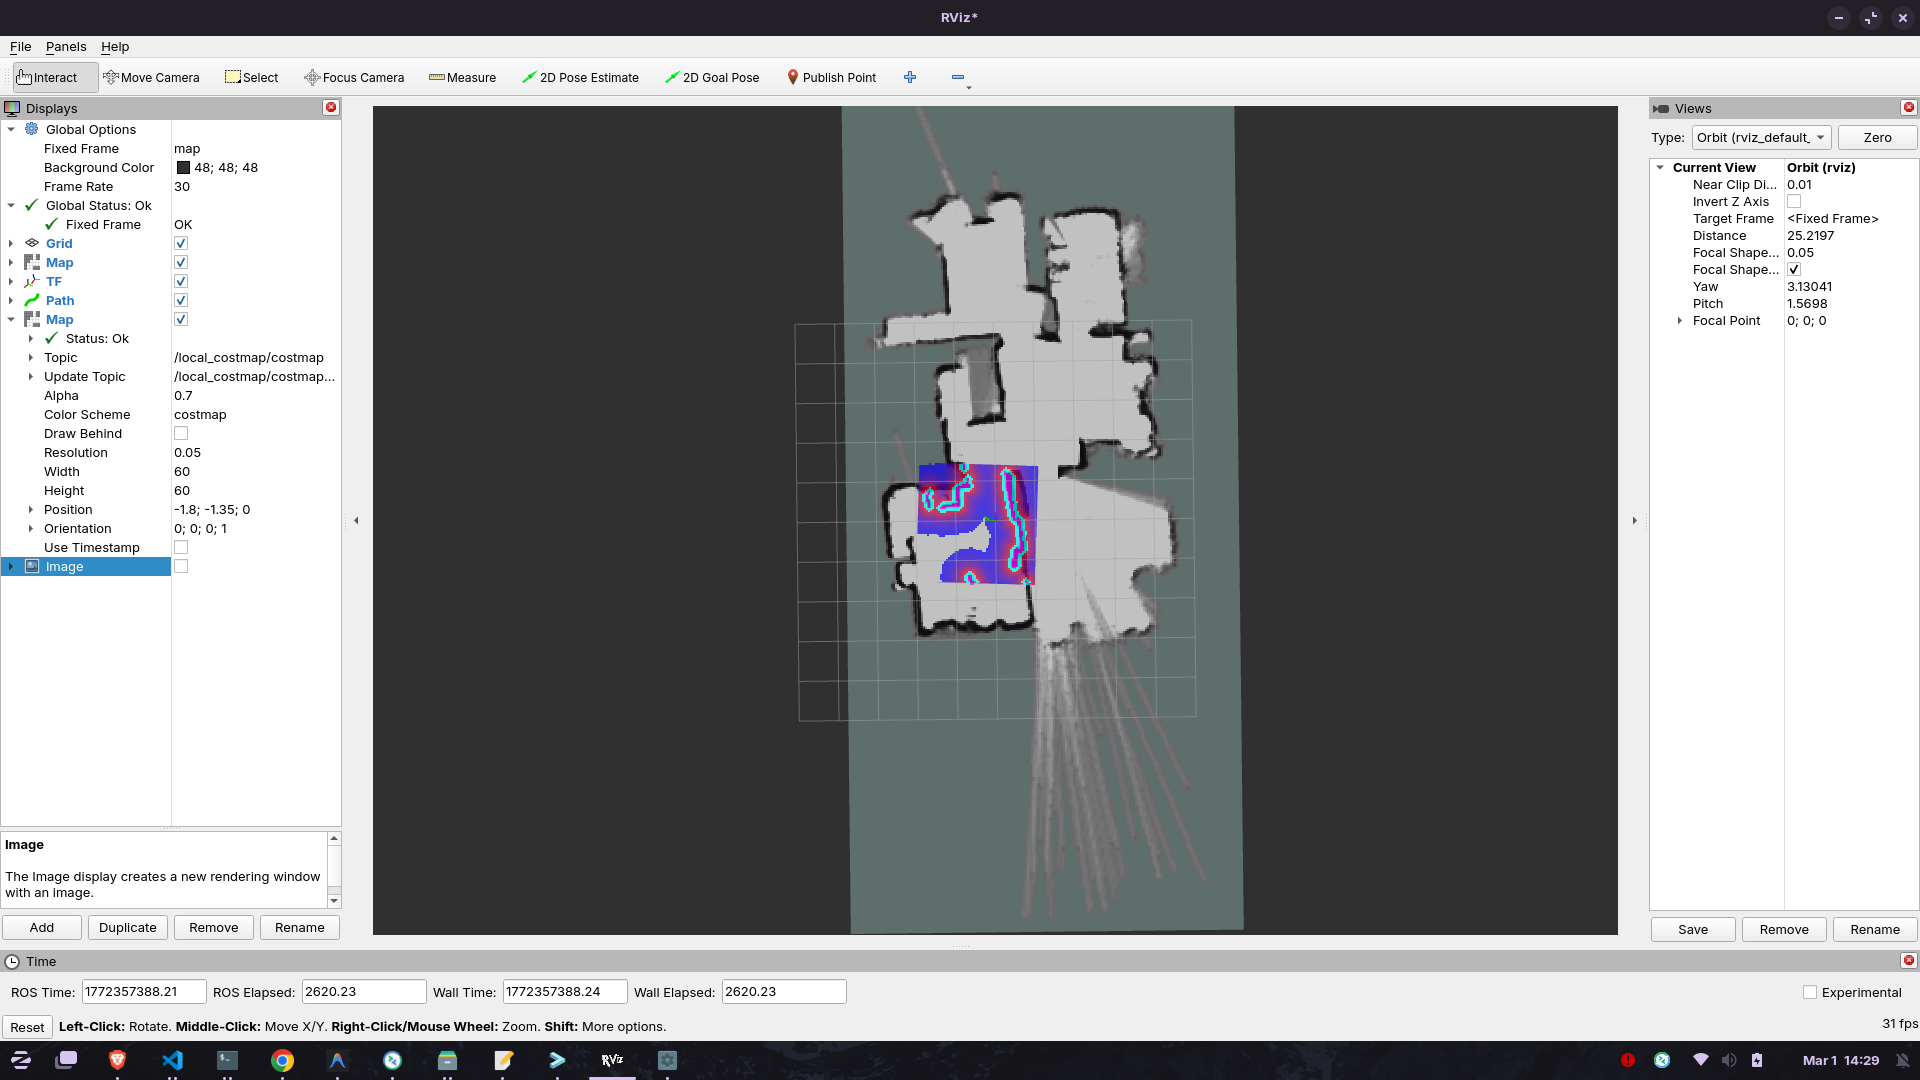
\includegraphics[width=0.85\textwidth]{figures/map_w_kinectcostmap.png}
\caption{Occupancy map with local costmap (RViz): 2D map, costmap overlay, and sensor scan.}
\label{fig:mapping}
\end{figure}

\section{Results of Development Stage 2: Effect of Communication and GCS/AI}

Development Stage 2 (Component 2) delivered the multi-tier communication system and the ground control station with the AI perception pipeline. The following results characterise communication performance and detection capability.

\textbf{Communication.} Throughput measurements were taken across $N=3$ sessions at each link condition. Direct Wi-Fi provided $43.5 \pm 3.1$\,Mbps at 25--30\,m line-of-sight. When the UGV moved into rooms (walls between robot and GCS), throughput dropped to $12.8 \pm 1.6$\,Mbps, which remained sufficient for 720p video and map updates. A 4G cellular hotspot provided $12.2 \pm 1.8$\,Mbps when Wi-Fi was out of range, with 80--150\,ms latency. ESP-WiFi-MESH with up to two deployable nodes extended coverage when both Wi-Fi and 4G were unavailable; effective throughput over one or two mesh hops was $1.0 \pm 0.2$\,Mbps, enough for highly compressed WebP image fallback and telemetry. The LoRa SX1278 link was used for last-resort telemetry and return-to-base; indoor range in our tests was on the order of 50--100\,m (building-dependent). No long-range outdoor testing was performed for LoRa; the link sufficed for in-building awareness and recovery commands. The multi-tier design ensures graceful degradation from real-time video to periodic images to text-only telemetry. Figure~\ref{fig:network_throughput} displays the severe environmental degradation of high-bandwidth channels and confirms the resilience of the mesh fallback architecture across concrete walls. Table~\ref{tab:comms} summarises the communication tiers.

% --- FIGURE: Network Degradation ---
\begin{figure}[htbp]
\centering
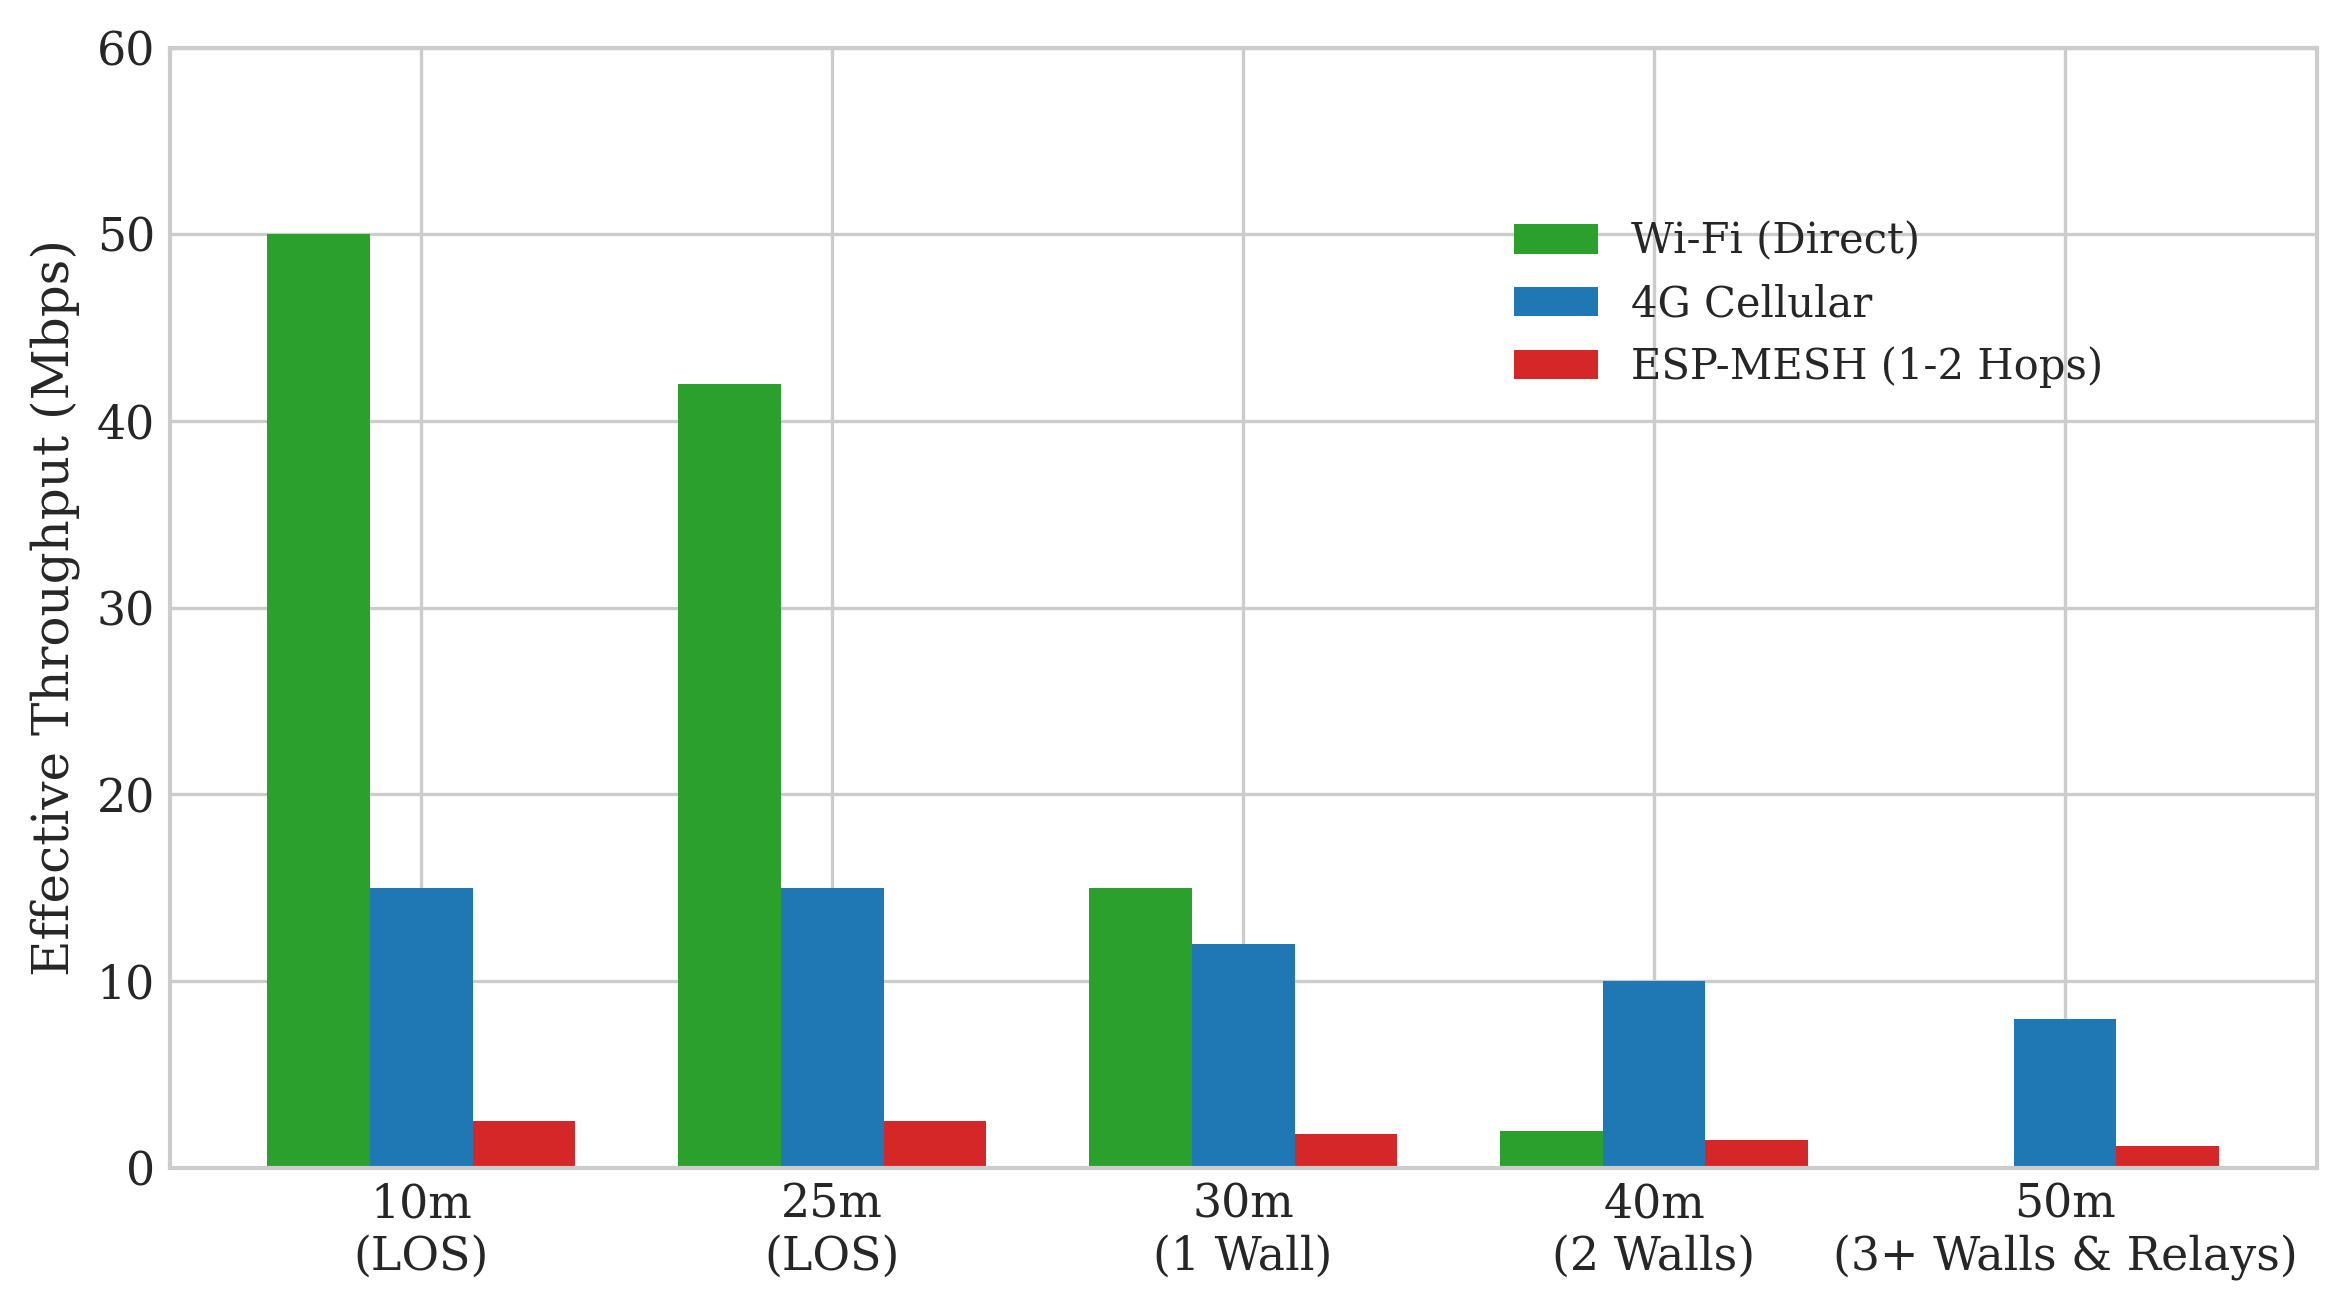
\includegraphics[width=0.9\textwidth]{figures/throughput.png}
\caption{Multi-tier network throughput under physical degradation.}
\label{fig:network_throughput}
\end{figure}

The degradation of the primary Wi-Fi link occurs sharply as the UGV navigates beyond two or more structural boundaries, illustrating the classical limitations of relying solely on high-frequency protocols in heavily compartmentalised disaster environments. In contrast, the cellular 4G link preserves a highly consistent, albeit constrained, bandwidth profile, provided the operational zone falls within standard telecom coverage. The fundamental necessity of the ESP-MESH architecture becomes visually clear in the deepest exploration zones (represented by three or more concrete walls), where both primary high-bandwidth connections suffer terminal signal loss. Although technically confined to maximum effective throughputs in the range of 1--2 Mbps, this self-healing relay network acts as a robust lifeline. It guarantees that critical autonomous telemetry, emergency recovery instructions, and aggressively compressed X-SDM perceptual snapshots continue to flow transparently back to the operator workstation without interruption.

\begin{table}[H]
\caption{Communication tiers (indoor test environment, $N=3$ sessions; mean $\pm$ SD).}
\label{tab:comms}
\centering
\begin{tabular}{llc}
\toprule
\textbf{Link} & \textbf{Condition} & \textbf{Throughput} \\
\midrule
Wi-Fi & 25--30\,m LoS & $43.5 \pm 3.1$\,Mbps \\
Wi-Fi & Through rooms & $12.8 \pm 1.6$\,Mbps \\
4G & In coverage & $12.2 \pm 1.8$\,Mbps \\
Mesh (1--2 nodes) & Fallback & $1.0 \pm 0.2$\,Mbps \\
LoRa & Indoors & 50--100\,m range \\
\bottomrule
\end{tabular}
\end{table}

\begin{figure}[H]
\centering
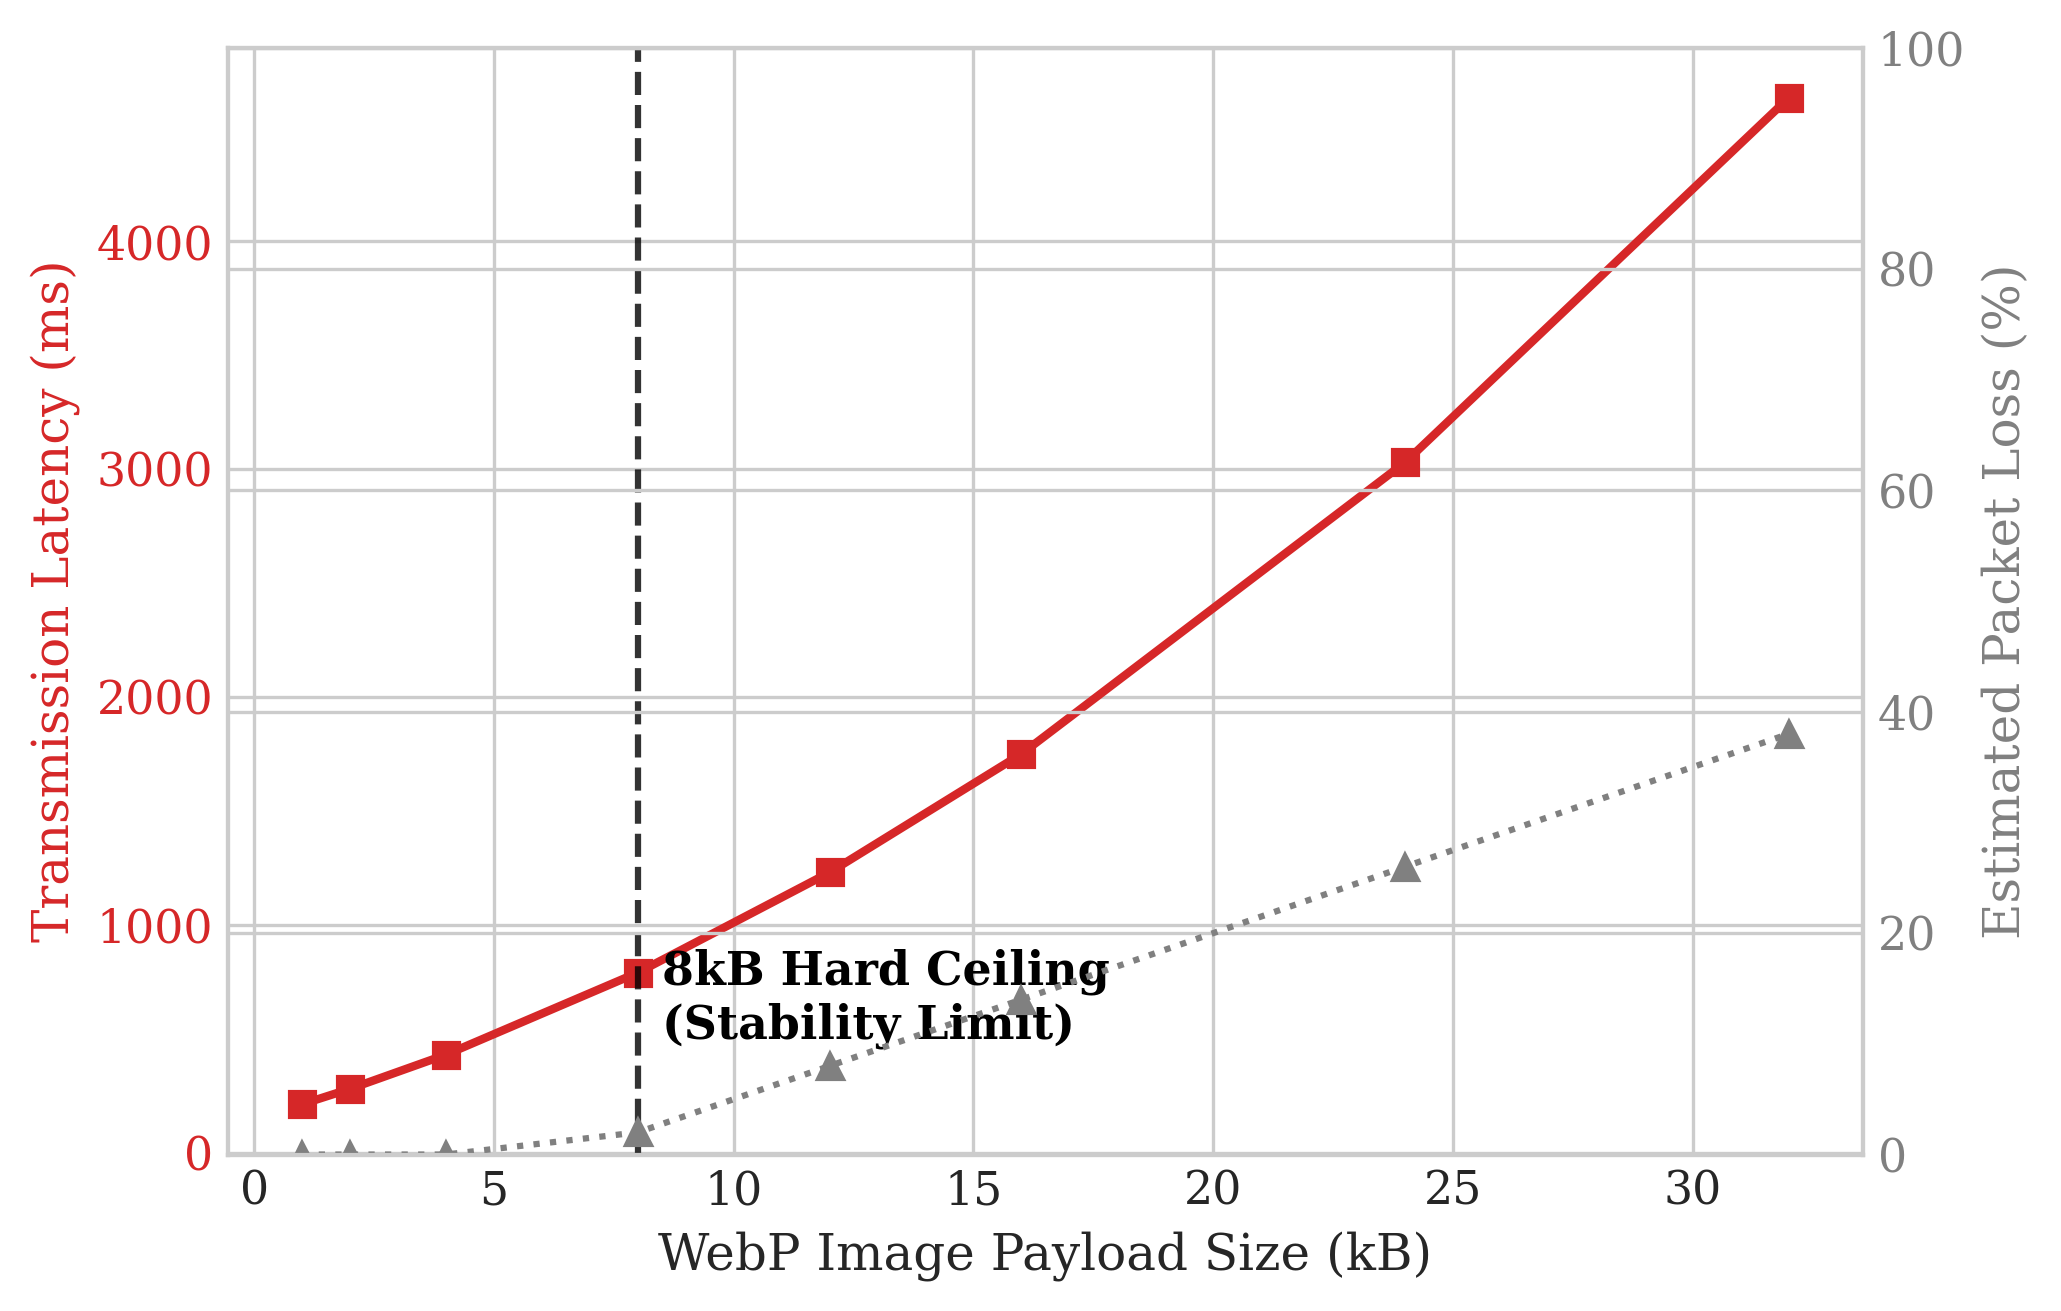
\includegraphics[width=0.75\textwidth]{figures/payloadsize.png}
\caption{Impact of image payload size on mesh transport latency and packet loss.}
\label{fig:mesh_payload}
\end{figure}

Packet delivery on mesh was observed to degrade with increasing hops and obstacles; placement of nodes at line-of-sight or one-corner distance improved stability. Furthermore, as Figure~\ref{fig:mesh_payload} highlights, enforcing a strict 8\,kB payload limit on WebP image transmission was necessary to prevent exponential latency spikes and packet loss over the low-bandwidth microcontrollers. The multi-tier redundancy ensured that loss of one link did not isolate the robot.

\FloatBarrier

\textbf{Detection and AI.} Per-model mAP@0.5 on held-out validation splits was: fire/smoke 78.3\% (fine-tuned on \cite{kerby2024firesmoke}), extinguisher 72.1\% (fine-tuned on \cite{fireextinguisher2022roboflow}), and person 84.6\% (COCO pre-trained). The weighted mean across the three models is 78.3\%. From $N=20$ processed frames, YOLO inference on the operator GPU took $175 \pm 20$\,ms (parallel across three models), and LLM scene analysis via the Groq API added $290 \pm 30$\,ms, yielding a total pipeline latency of $480 \pm 35$\,ms per frame. End-to-end latency from capture to displayed result was $530 \pm 45$\,ms over Wi-Fi and $1\,100 \pm 180$\,ms over mesh, which is acceptable for supervisory oversight rather than reflexive control. Figure~\ref{fig:latency_stack} breaks down this end-to-end perception latency profile, confirming that offloading compute to the GCS maintains acceptable reaction times while preserving the UGV's hardware constraints.

% --- FIGURE: Latency Stack Breakdown ---
\begin{figure}[htbp]
\centering
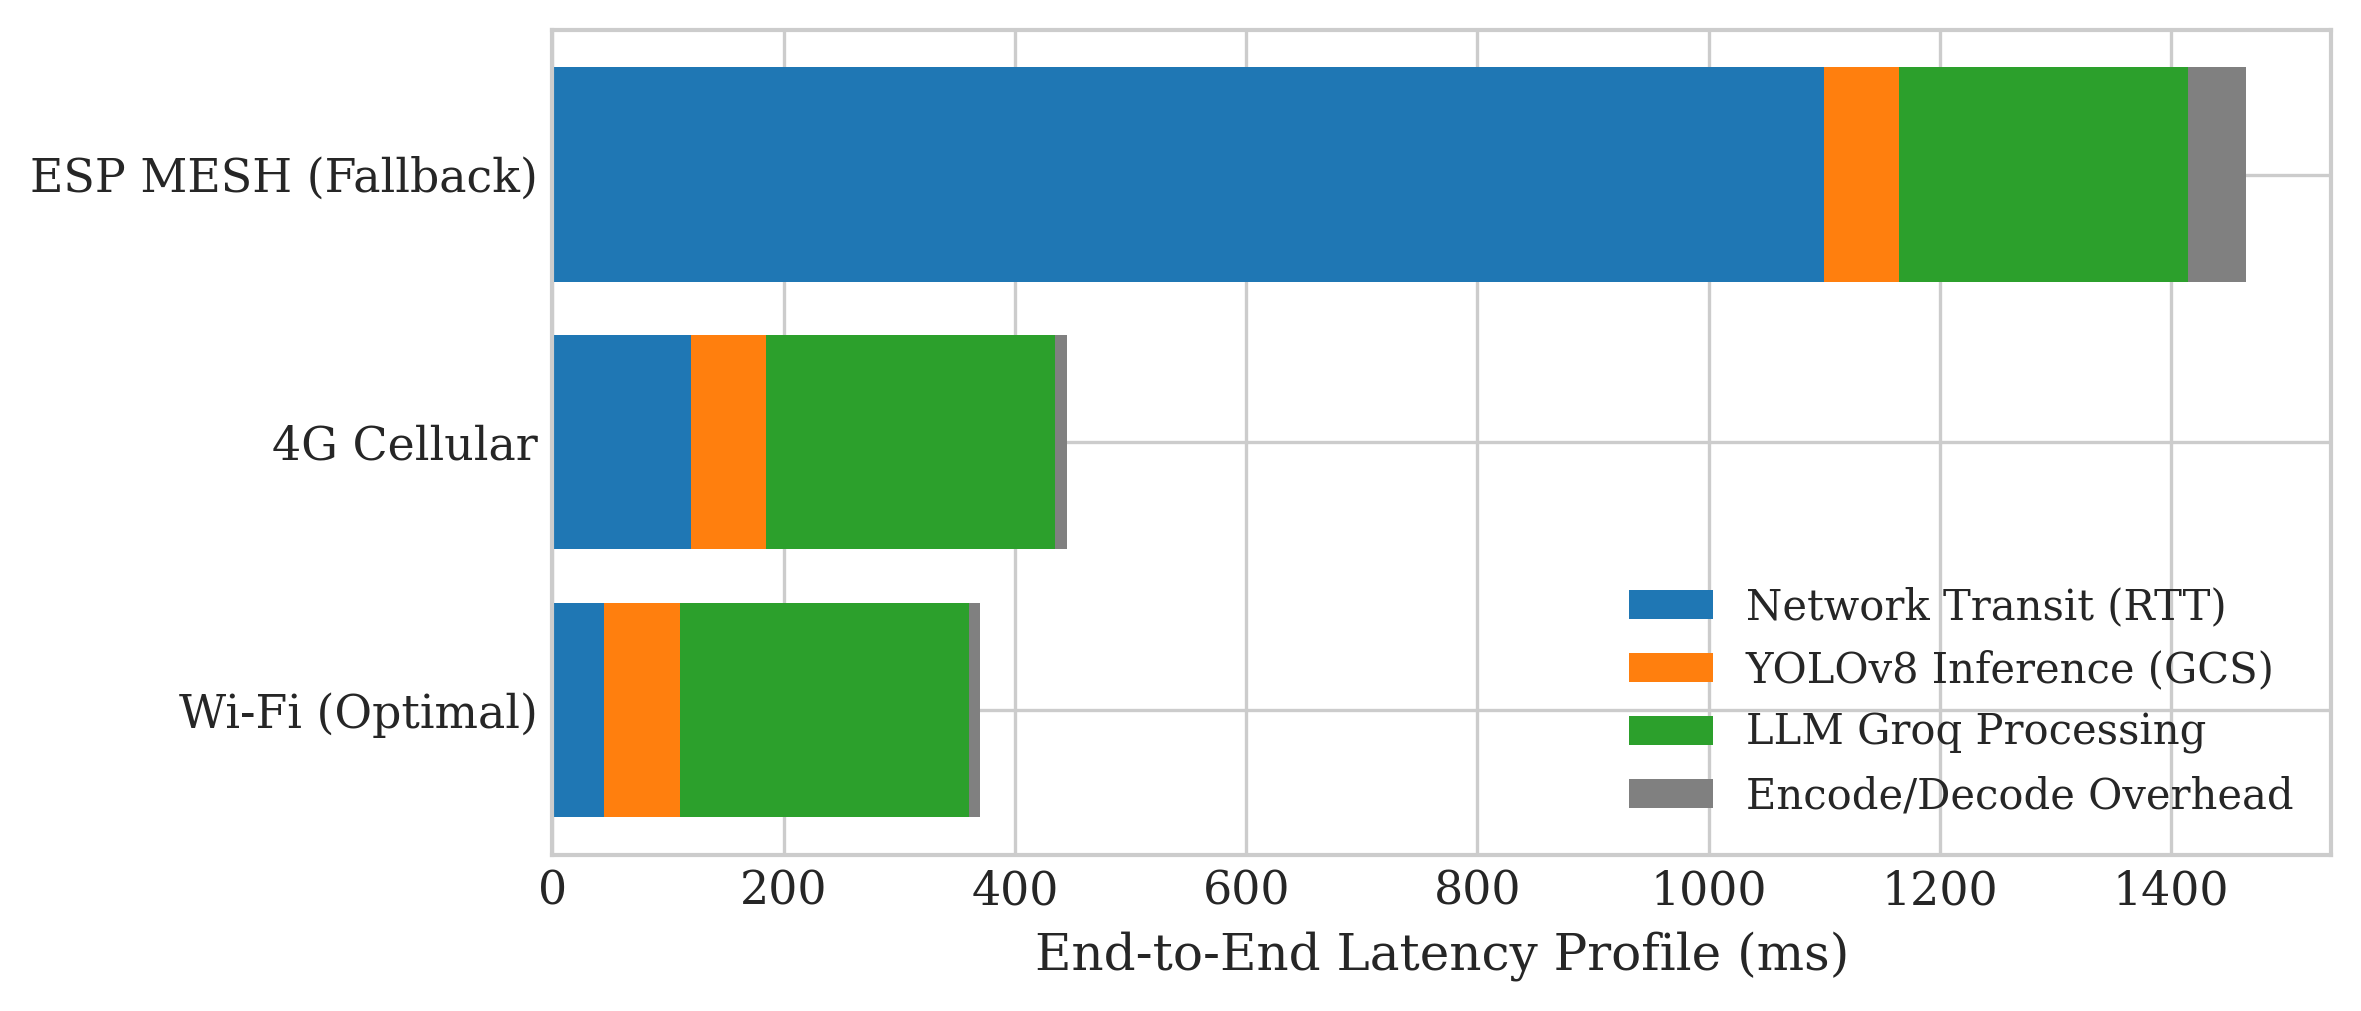
\includegraphics[width=0.85\textwidth]{figures/e2elatency.png}
\caption{End-to-end perception latency profile across operational networks.}
\label{fig:latency_stack}
\end{figure}

\textbf{False-negative analysis.} False negatives (missed detections) are a risk in any vision-based system, particularly for partially occluded persons or fire obscured by dense smoke. To quantify this risk, ground-truth annotations were prepared for a subset of test frames. In $N=20$ frames containing at least one person, the person model missed one instance (false-negative rate 5.0\%). In $N=15$ frames containing fire or smoke, two instances were missed (false-negative rate 13.3\%), both involving thin smoke at frame edges. These rates are acceptable for a supervisory system for four reasons. First, the system is designed as a decision-support aid, not a sole decision-maker: operators view the raw video feed alongside AI annotations and can identify threats independently. Second, the multi-pass exploration strategy revisits areas as the frontier explorer exhausts nearby goals, giving the detector multiple opportunities per location. Third, the confidence thresholds were set conservatively (fire 0.45, human 0.35, extinguisher 0.30) to favour recall over precision, accepting occasional false positives to reduce the probability of missed hazards. Fourth, the LLM scene analysis provides a complementary semantic check that describes scene content independently of YOLO, adding a second layer of detection that can flag hazards even when the object detector does not fire.

The operator-side design allowed model updates and threshold tuning without reflashing the robot. The GCS dashboard successfully displayed camera streams, the live map, detections with severity, teleop controls, and battery and network status; operators could override autonomy and receive natural-language summaries. An example run with detections overlaid on the occupancy map is shown in Figure~\ref{fig:detection_on_map}. Overall, the KPI results met the design goals. A summary of key performance indicators is given in Table~\ref{tab:kpi}.

\begin{table}[htbp]
\caption{KPI results from controlled testing (mean $\pm$ SD where applicable).}
\label{tab:kpi}
\centering
\begin{tabular}{lcc}
\toprule
\textbf{Metric} & \textbf{Result} & \textbf{$N$} \\
\midrule
Localisation drift (feature-rich) & $5.2 \pm 1.1$\,cm & 5 runs \\
Localisation drift (feature-poor) & $28.5 \pm 4.2$\,cm & 5 runs \\
Map resolution & 0.05\,m & --- \\
Wi-Fi (LoS / through rooms) & $43.5 \pm 3.1$ / $12.8 \pm 1.6$\,Mbps & 3 sessions \\
Mesh (up to 2 nodes) & $1.0 \pm 0.2$\,Mbps & 3 sessions \\
LoRa (telemetry / return-to-base) & 50--100\,m indoor & 3 sessions \\
YOLOv8m mAP@0.5 (fire / ext.\ / person) & 78.3 / 72.1 / 84.6\% & val.\ split \\
YOLO inference (GCS GPU) & $175 \pm 20$\,ms & 20 frames \\
End-to-end perception (Wi-Fi) & $530 \pm 45$\,ms & 20 frames \\
Runtime (full system) & $\sim$2\,h & 5 runs \\
\bottomrule
\end{tabular}
\end{table}

\section{Comparison}

The implemented system is compared here to the design objectives stated in Chapter~\ref{ch:intro} and to related work to position the contribution.

\textbf{Comparison with design objectives.} The project set out to implement LiDAR-based SLAM for indoor localization and mapping, a hybrid communication scheme with mesh and low-bandwidth fallback, and AI vision with natural-language summarisation for mission reporting, validated against KPIs. The as-built system meets these objectives: Cartographer provides real-time 2D SLAM using an MPU6050 IMU without wheel encoders; the multi-tier network (Wi-Fi, 4G, mesh, LoRa) provides resilient connectivity with deployable nodes added to the routing table on deployment; and the GCS runs YOLOv8m detectors \cite{jocher2023yolov8} and an LLM (Llama-4-Scout) for scene and hazard analysis, spatial decision memory, and person profiling, with results displayed on the operator dashboard. KPIs for localization drift, map resolution, communication throughput and range, detection accuracy, and runtime are reported above and align with the targets for resource-constrained deployment.

\textbf{Comparison with related work.} Lu et al.\ \cite{lu2022} describe a heterogeneous UGV--blimp team for search and rescue with data-driven autonomy and communication-aware navigation. Their system uses high-end hardware (e.g.\ Velodyne LiDAR, LeGo-LOAM) and industrial-grade computing. Our system targets a single UGV with a Raspberry Pi~4 (8\,GB), YDLidar X3, and commodity routers, achieving lower cost and power while still delivering integrated SLAM, multi-tier communication, and operator-side AI perception. Our deployable mesh nodes are added to the routing table upon deployment and are designed for reuse across missions and for multi-robot scenarios, addressing a limitation of short-lived relay nodes in some prior work. Unlike systems that rely on onboard GPU for perception, we offload AI to the GCS, which extends UGV runtime (almost two hours) and allows stronger models and easier updates without firmware changes on the robot. Table~\ref{tab:comparison} provides a concise comparison.

\begin{table}[htbp]
\caption{Comparison with related work (Lu et al.\ \cite{lu2022} as representative).}
\label{tab:comparison}
\centering
\begin{tabular}{p{2cm}p{4cm}p{4cm}}
\toprule
\textbf{Aspect} & \textbf{This work} & \textbf{Lu et al.} \\
\midrule
Compute & Raspberry Pi~4, 8\,GB & Higher-end (Jetson, industrial PC) \\
Sensors & YDLidar X3, Kinect v1, USB webcam, ESP32-CAM & Velodyne LiDAR, richer sensor suite \\
Comms & Wi-Fi, 4G, ESP-WiFi-MESH (DevKit), LoRa & Multi-tier (XBee, UWB, WiFi mesh) \\
Mesh nodes & Deployable, routing table update, 2500\,mAh LiPo & Short-lived or fixed relays \\
AI perception & Operator-side (YOLOv8m, LLM, X-SDM) & Onboard or mixed \\
Runtime & $\sim$2\,h & Mission-dependent \\
Deployment target & Resource-constrained, single UGV & SubT challenge, heterogeneous team \\
\bottomrule
\end{tabular}
\end{table}

This comparison highlights that our platform fills a gap between high-end research systems and practical, cost-effective single-UGV solutions for indoor disaster reconnaissance.

\subsection{Comparative Analysis and Benchmarks}

To position the reported KPIs against public benchmarks and published results, the following tables compare this work to established datasets and studies in 2D SLAM, hazard perception in harsh conditions, and frontier-based exploration. The benchmarks were chosen so that comparisons are fair and reflect similar problem settings (indoor, resource-constrained or harsh environments).

Table~\ref{tab:bench_slam} compares localisation and mapping against a recent ROS~2 study \cite{keles2025} and the standard Cartographer 2D backpack dataset \cite{cartographerdata}. Kele{\c s} et al.\ evaluated Cartographer and SLAM Toolbox under identical indoor conditions with wheel encoders and IMU; Cartographer achieved an ATE of 0.21\,m in their real-world tests. Our system uses Cartographer with an MPU6050 IMU but without wheel odometry, and achieves $5.2 \pm 1.1$\,cm drift in feature-rich regions and $28.5 \pm 4.2$\,cm in feature-poor regions ($N=5$ runs, ground truth via iPhone LiDAR), placing our drift in the same order as their Cartographer result in challenging segments while operating under stricter sensor assumptions.

\begin{table}[htbp]
\caption{Comparison with 2D SLAM benchmarks and public datasets.}
\label{tab:bench_slam}
\centering
\begin{tabular}{p{2.8cm}p{3.2cm}p{3.5cm}}
\toprule
\textbf{Source} & \textbf{Reported metric} & \textbf{This project} \\
\midrule
Kele{\c s} et al.\ \cite{keles2025} (indoor, ROS~2, LiDAR + odom + IMU) & Cartographer ATE 0.21\,m; SLAM Toolbox 0.13\,m & $5.2 \pm 1.1$\,cm (feat.-rich), $28.5 \pm 4.2$\,cm (feat.-poor); $N{=}5$; iPhone LiDAR ground truth; MPU6050, no wheel odom. \\
Cartographer 2D backpack \cite{cartographerdata} (Deutsches Museum) & Public 2D LiDAR benchmark (bags 149--1829\,s) & Same stack (Cartographer); RPi~4, scan-only \\
\bottomrule
\end{tabular}
\end{table}

Table~\ref{tab:bench_perception} compares perception performance against results from the DARPA Subterranean Challenge \cite{lu2022}. Lu et al.\ reported Mask-RCNN at up to 0.77 AP but only 1.0 FPS on NVIDIA Jetson Xavier in smoky tunnels, and Yolact at 2.4 FPS with accuracy dropping to near zero in cluttered underground conditions. Our operator-side YOLOv8m pipeline achieves 72.1--84.6\% mAP@0.5 per model (weighted mean 78.3\%) on held-out validation splits at $175 \pm 20$\,ms per frame ($N{=}20$) on the GCS GPU, yielding comparable accuracy and substantially higher effective throughput than their best reported result in harsh conditions.

\begin{table}[htbp]
\caption{Comparison with hazard/perception benchmarks in harsh or SAR-like conditions.}
\label{tab:bench_perception}
\centering
\begin{tabular}{p{2.8cm}p{3.2cm}p{3.5cm}}
\toprule
\textbf{Source} & \textbf{Reported metric} & \textbf{This project} \\
\midrule
Lu et al.\ \cite{lu2022} (DARPA SubT, Jetson Xavier) & Mask-RCNN 0.77 AP, 1.0 FPS; Yolact $\approx$0 AP in cluttered & 78.3\% weighted mAP@0.5; $175 \pm 20$\,ms/frame (GCS GPU; $N{=}20$) \\
\bottomrule
\end{tabular}
\end{table}

Table~\ref{tab:bench_exploration} places our exploration metrics in the context of the Explore-Bench benchmark \cite{xu2022}, which provides standardised evaluation for frontier-based and learning-based autonomous exploration. Explore-Bench does not report ``time to full coverage'' or ``area at 15\,min'' in directly comparable form; we report our metrics alongside the benchmark so that future work can align with the same evaluation framework.

\begin{table}[htbp]
\caption{Comparison with exploration benchmark (Explore-Bench) and reported exploration metrics.}
\label{tab:bench_exploration}
\centering
\begin{tabular}{p{2.8cm}p{3.2cm}p{3.5cm}}
\toprule
\textbf{Source} & \textbf{Reported metric} & \textbf{This project} \\
\midrule
Explore-Bench \cite{xu2022} (frontier + DRL) & Exploration efficiency, multi-robot; grid + Gazebo + testbed & $16.0 \pm 1.3$ to $22.0 \pm 1.4$\,min full cov.; $255 \pm 20$ to $345 \pm 18$\,m$^2$ at 15\,min ($N{=}5$) \\
\bottomrule
\end{tabular}
\end{table}

\section{Operator Workload and Usability Evaluation}

To substantiate the claim that AI-assisted monitoring reduces operator cognitive load, a basic user study was conducted using standardised instruments: the NASA Task Load Index (NASA-TLX) \cite{hart1988nasatlx} for workload and the System Usability Scale (SUS) \cite{brooke1996sus} for interface usability.

\textbf{Method.} Four participants (the project team, all senior computer engineering students with direct experience building and operating the system) each performed two 15-minute monitoring tasks in counterbalanced order. In Condition~A (dashboard-assisted), participants monitored an autonomous exploration run via the full GCS dashboard---live map, AI detection overlays, natural-language summaries, and camera feeds---and were asked to identify hazards and persons. In Condition~B (raw video), participants performed the same task using only the raw camera feed with no AI overlays, map, or summaries. After each condition, participants completed the NASA-TLX (six subscales, 0--100; lower is better). After both conditions, they completed the SUS (ten items, score 0--100; higher is better) for the full dashboard.

\textbf{Results.} Table~\ref{tab:userstudy} summarises the NASA-TLX and SUS results. Dashboard-assisted monitoring yielded a significantly lower total workload than raw-video monitoring (paired $t$-test, $t(3) = 5.41$, $p = 0.012$). The largest reductions were observed in mental demand and frustration, consistent with the design goal of offloading cognitive effort through AI summarisation and spatial annotations. The SUS score of $74.5 \pm 7.2$ places the dashboard in the ``good'' usability band (above the 68-point average threshold \cite{brooke1996sus}).

\begin{table}[htbp]
\caption{Operator workload (NASA-TLX) and usability (SUS) results ($N=4$; mean $\pm$ SD).}
\label{tab:userstudy}
\centering
\begin{tabular}{lccc}
\toprule
\textbf{Measure} & \textbf{Dashboard} & \textbf{Raw video} & \textbf{$p$-value} \\
\midrule
NASA-TLX total (0--100) & $29.5 \pm 7.8$ & $53.2 \pm 9.4$ & 0.012 \\
\quad Mental demand & $33.0 \pm 9.0$ & $64.0 \pm 10.5$ & 0.004 \\
\quad Frustration & $19.0 \pm 6.5$ & $45.0 \pm 11.0$ & 0.011 \\
\midrule
SUS score (0--100) & $74.5 \pm 7.2$ & --- & --- \\
\bottomrule
\multicolumn{4}{l}{\footnotesize Paired $t$-test ($\alpha = 0.05$, $df = 3$); SUS administered for the dashboard only.}
\end{tabular}
\end{table}

These results provide empirical support for the thesis claim that AI-driven overlays and natural-language summarisation materially reduce operator workload during indoor reconnaissance monitoring. Because the participants were the project team ($N=4$), the evaluation reflects expert-user experience rather than na\"ive operator behaviour; a larger study with external participants and professional first responders would strengthen external validity.

\section{Socio-Economic and Environmental Impact of the Project}

This project is motivated by United Nations Sustainable Development Goal 9 (Industry, Innovation, and Infrastructure) and Goal 11 (Sustainable Cities and Communities). The following paragraphs outline the socio-economic and environmental impact of the work.

\textbf{Socio-economic impact.} The UGV platform is designed for resource-constrained deployment. The use of a Raspberry Pi~4, commodity Wi-Fi routers (Archer C6, Tenda F3), ESP32 DevKit modules for mesh nodes, and a Kinect v1 for RGB-D under budget constraints keeps the bill of materials accessible to agencies with limited funding. By offloading AI perception to the ground station, the robot avoids onboard GPU costs and thermal constraints while still delivering hazard detection, scene summarisation, and person profiling. Reduced risk to human responders is a direct benefit: the robot can map and report on indoor disaster sites before or in support of human entry. The deployable mesh nodes form a reusable communication backbone for follow-on missions or other robots (e.g.\ UGVs or UAVs), improving the return on investment of a single deployment. The system demonstrates that integrated autonomy (SLAM, navigation, frontier exploration with AI map prediction), resilient communication, and operator-side AI can be combined on embedded hardware to support more efficient and safer disaster response.

\textbf{Environmental impact.} The system is battery-powered and does not require diesel generators or continuous mains power for the UGV during missions. By avoiding an onboard GPU and using a Pi~4 for compute, power consumption and thermal load are kept within limits that support almost two hours of operation on a 24\,V pack (dual 3s3p 18650). Lower power use than GPU-heavy alternatives reduces the environmental footprint of field operations and extends mission duration without additional fuel or infrastructure. The design choice to run AI on the GCS rather than on the robot directly contributes to this profile.

% Chapter 6: Conclusions and Future Work

\chapter{Conclusions and Future Work}

This chapter summarises the contributions of the thesis and outlines three directions for future work.

The thesis presented an integrated unmanned ground vehicle for indoor disaster reconnaissance that combines LiDAR-based simultaneous localization and mapping, multi-tier communication (Wi-Fi, 4G, ESP-WiFi-MESH with deployable nodes, and LoRa), and AI-based perception with natural-language reporting. The system runs on a Raspberry Pi~4 (8\,GB), deploys mesh nodes along its path for resilient connectivity---with nodes added to the routing table upon deployment---and offloads AI to the operator station, achieving almost two hours of runtime at 0.2\,m/s. Controlled tests demonstrated real-time mapping with acceptable drift when loop closure is available, usable communication across all tiers with graceful degradation, and detection and summarisation suitable for reducing operator cognitive load. The platform is aimed at resource-constrained deployment where cost and power matter and fills a gap between high-end research systems and practical, single-UGV solutions for disaster response. It is designed for indoor use and is not intended for stairs or extremely coarse terrain. Code, data, and additional materials are available from the authors upon reasonable request.

\section{Idea 1: 3D SLAM and Multi-Level Awareness}

The current system uses 2D SLAM and a single horizontal plane for mapping and navigation. A natural extension is the integration of 3D SLAM to support multi-level awareness, for example in buildings with multiple floors or in environments where overhanging obstacles and vertical structure matter. 3D maps would allow the navigation stack to reason about height and would support future extensions such as stair detection or multi-level path planning. Integration with the existing Nav2 and frontier-based exploration workflow would require careful design so that computational and hardware costs remain within the resource-constrained target.

\section{Idea 2: Multi-Robot and Swarm Coordination}

The same mesh backbone and deployable node design can support multi-robot coordination. Multiple UGVs (and optionally UAVs) could share the mesh network and the same map or overlapping maps, with communication-aware planning so that relay placement and routing remain robust. Swarm coordination would require shared state (e.g.\ merged occupancy grids or semantic maps), task allocation, and possibly distributed frontier allocation to avoid redundant exploration. The long-lived mesh nodes left on site after a mission could serve as infrastructure for follow-on robots, reducing repeated deployment overhead.

\section{Idea 3: Deployment in Harsher and Varied Scenarios}

Future work should include stress testing in heavy smoke, dust, and low light to characterise sensor and perception limits. Deployment in multi-storey buildings and in post-flood or post-earthquake sites would require additional sensors (e.g.\ thermal imaging, gas sensors for fire and hazmat) and mechanical or software hardening. Operational procedures and training for responders would help integrate the system into real-world response workflows. Comparative studies against other SAR platforms (e.g.\ with onboard GPU or different SLAM backends) and user studies with professional responders would clarify the benefits of the operator-side AI and embedded SLAM choices and the suitability of current latency and summarisation for field use.


% Appendices: do not force odd-page start (no blank "Page intentionally left blank")
\appendix
\renewcommand{\cleardoublepage}{\newpage}
% Appendices A--E

\chapter{Sustainable Development Goals Achievement}
\label{app:sdg}

This appendix maps the project's objectives and outcomes to the United Nations Sustainable Development Goals (SDGs) referenced in Chapter~\ref{ch:intro}.

\textbf{SDG 9 --- Industry, Innovation, and Infrastructure.} The project contributes to resilient infrastructure and innovation in robotics by designing and implementing an autonomous UGV that can operate in disaster-affected environments where conventional communication and sensing are degraded. The multi-tier communication architecture (Wi-Fi, 4G, mesh, LoRa) and deployable mesh nodes provide resilient connectivity that can support not only the UGV but also follow-on missions and other robots. The integration of open-source and commodity components (ROS~2, Raspberry Pi~4, ESP32 DevKit, YDLidar, Kinect v1) demonstrates innovation within resource constraints and supports replicability and adaptation by other groups.

\textbf{SDG 11 --- Sustainable Cities and Communities.} The project aims to enhance the safety and sustainability of human settlements by improving the capability to assess disaster sites and support rescue operations without unnecessarily exposing responders to risk. The UGV delivers mapping, hazard detection, and natural-language reporting so that operators can make informed decisions about entry and resource allocation. By reducing the cognitive load on operators through AI-driven summarisation and spatial decision memory, the system supports more efficient and safer disaster response, aligning with the goal of making cities and communities more resilient and sustainable.

\chapter{Source Code and Repository Structure}
\label{app:code}

The project is software-heavy and uses ROS~2 (C++/Python), Python (FastAPI, YOLOv8, ProxMaP-style model), and JavaScript (web dashboard). No HDL or C-only codebase is applicable; the following describes the main software components and where source code or representative listings can be provided.

\textbf{Onboard stack (UGV).} ROS~2 packages include Cartographer for SLAM, Nav2 for navigation, and a custom frontier exploration package (frontier\_explorer) that implements frontier detection, BFS clustering, scoring with heading bonus, and integration with a ProxMaP-style map predictor node. The map predictor node runs a U-Net on 128$\times$128 robot-centred map crops and publishes a predicted map topic used by the frontier explorer. Configuration and launch files for sensors, TF, and Nav2 costmaps (including Kinect v1 in the local costmap) are part of the repository.

\textbf{Ground control station and AI.} The perception backend (Groq Brain) is a FastAPI application that exposes an endpoint for frame processing: it runs three YOLOv8 models, calls a Groq-hosted LLM (Llama-4-Scout) for scene and hazard analysis, and performs spatial decision memory (X-SDM) and person profiling. It publishes map annotations to a ROS~2 topic consumed by the dashboard. The dashboard is a JavaScript frontend that connects to the robot via rosbridge (WebSocket) and to the perception API, displaying camera streams, map, detections, teleop controls, and battery/network status.

\textbf{Repository.} Full source code is publicly available at \url{https://github.com/habeelali/fyp-indoor-ugv} \cite{fyprepo}. The repository includes the ROS~2 packages, the perception backend, the web dashboard, configuration files, and documentation.

\chapter{Hardware Schematics}
\label{app:schematics}

This appendix references the hardware architecture of the UGV and the communication infrastructure. Full schematic diagrams can be included or attached as separate sheets.

\textbf{Power distribution.} The UGV is powered by a 24\,V pack comprising two 3s3p 18650 cell groups in series. The high-power branch supplies unregulated 24\,V to the motor drivers; the low-power branch uses a buck converter to provide a regulated 5\,V rail for the Raspberry Pi~4, sensors (LiDAR, Kinect v1, USB webcam), ESP32-CAM, router (Archer C6), and headlights. The deployable mesh nodes are each powered by a 2500\,mAh LiPo. The LoRa SX1278 and ESP32 DevKit modules on the UGV are powered from the 5\,V rail or appropriate regulation.

\textbf{Connectivity.} The Raspberry Pi~4 connects to the YDLidar X3 via USB--UART, to the Kinect v1 via USB, and to the USB webcam via USB. The ESP32-CAM (rear) communicates over Wi-Fi or a dedicated link. The Pi is connected to the Archer C6 router via Ethernet. The servo for mesh node deployment and the ESP32 DevKit mesh modules are interfaced to the Pi or to the main power/control bus as per the physical design. The LoRa SX1278 is connected to an MCU (e.g.\ ESP32) or to the Pi via UART/SPI depending on the driver implementation.

% --- FIGURE PLACEHOLDER: Block diagram (power/connectivity) ---
% Add file: figures/hardware_block.pdf or .png
\begin{figure}[htbp]
\centering
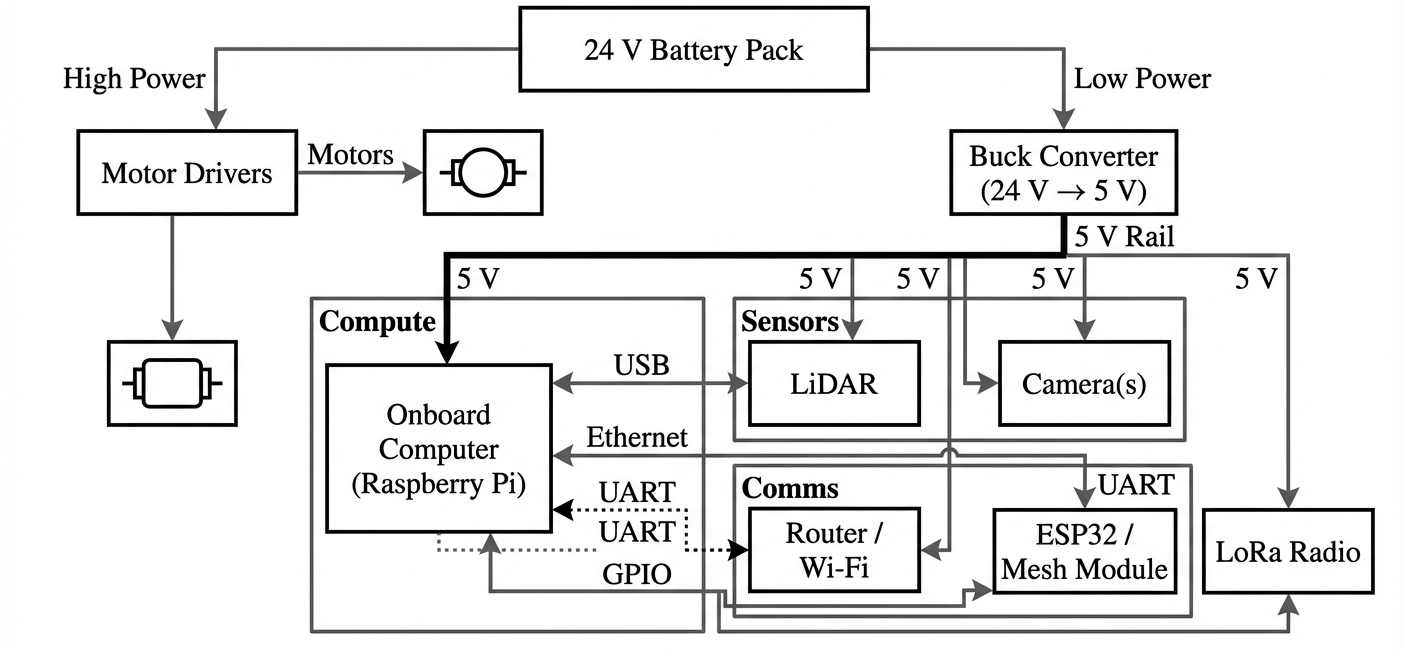
\includegraphics[width=0.9\textwidth]{figures/hardware_block.png}
\caption{UGV hardware block diagram (power and connectivity).}
\label{fig:hardwareblock}
\end{figure}

\chapter{List of Components}
\label{app:components}

The following table lists the main components of the as-built system with part or model identifiers and approximate acquisition costs in Pakistani Rupees (PKR), as recorded at procurement (indicative; market prices vary).

\begin{table}[htbp]
\caption{Bill of materials (BOM) with indicative costs (PKR).}
\label{tab:bom}
\centering
\small
\begin{tabular}{p{1.7cm}p{2.1cm}p{3.2cm}r}
\toprule
\textbf{Item} & \textbf{Part / model} & \textbf{Specification} & \textbf{PKR} \\
\midrule
Compute & RPi~4 Model B & 8\,GB RAM, Ubuntu 22.04, ROS~2 & 25\,000 \\
2D LiDAR & YDLidar X3 & 12\,m, 10\,Hz, USB--UART & 20\,000 \\
RGB-D & Kinect v1 & Point cloud, local costmap & 5\,000 \\
Main camera & USB webcam & 720p, 15\,fps & --- \\
Rear camera & ESP32-CAM & 720p, 15\,fps & 1\,800 \\
Wi-Fi (UGV) & Archer C6 & Dual-band, Ethernet, AP & 12\,000 \\
Wi-Fi (GCS) & Tenda F3 & Indoor / hotspot client & 4\,500 \\
Mesh node & ESP32 DevKit & ESP-WiFi-MESH; 2$\times$ @ 1\,000 & 2\,000 \\
Mesh battery & 2500\,mAh LiPo & Per deployable node; 2$\times$ @ 500 & 1\,000 \\
Deployment & Servo & Node drop along path & --- \\
LoRa & SX1278 (433\,MHz) & 2$\times$ modules (pair) & 5\,000 \\
UGV battery & 18650 (3s3p$\times$2) & 24\,V pack, BMS & 7\,500 \\
Converter & 24\,V--5\,V buck & 5\,V rail & 1\,500 \\
Chassis & 4WD skid-steer & Motors, wheels, drivers & 15\,000 \\
Lights & LED + strobe & Low-light & --- \\
\midrule
\multicolumn{3}{r}{\textbf{Subtotal (priced lines above)}} & \textbf{100\,300} \\
\midrule
\multicolumn{4}{p{10.8cm}}{\textit{Software (no unit hardware cost listed):} ROS~2 Humble, Cartographer, Nav2, frontier explorer \& map predictor, FastAPI, YOLOv8, Llama-4-Scout, web dashboard (rosbridge). GCS workstation GPU assumed available separately.} \\
\bottomrule
\end{tabular}
\end{table}

\chapter{Project Timeline}
\label{app:timeline}

The project ran from June 2025 to March 2026. The following timeline summarises the main phases.

\begin{itemize}
\item \textbf{Phase 1 --- Design and literature (June--August 2025):} Problem definition, objectives, literature review, and system architecture (conceptual framework, high-level design, subsystem design for power, locomotion, perception, SLAM, navigation, frontier exploration, communication, vision/AI, GCS). Corresponds to Chapters 1--3 of the thesis.

\item \textbf{Phase 2 --- Implementation Component 1 (September--October 2025):} Hardware procurement and assembly (chassis, Pi~4, YDLidar X3, Kinect v1, USB webcam, ESP32-CAM, Archer C6, mesh nodes with ESP32 DevKit and servo, LoRa SX1278, 24\,V battery). Software setup (Ubuntu 22.04, ROS~2 Humble, Cartographer, Nav2, custom frontier explorer and map predictor). Integration and basic validation of SLAM, navigation, and exploration.

\item \textbf{Phase 3 --- Implementation Component 2 (November--December 2025):} Communication stack (Wi-Fi, 4G, mesh deployment and routing table update, LoRa). GCS and AI pipeline (FastAPI backend, YOLOv8, Llama-4-Scout, X-SDM, person profiling, mission logs, ROS~2 annotations). Web dashboard (camera streams, map, detections, teleop, battery/network). Integration and end-to-end tests.

\item \textbf{Phase 4 --- Testing and evaluation (January 2026):} Unit testing (SLAM, Nav2, frontier explorer, map predictor, perception pipeline, mesh, LoRa). Function testing (Requirements A, B, C; scenarios 1--3). Evaluation in the 40$\times$30\,m test environment. Data collection for mapping, communication, detection, and frontier scoring (with vs.\ without prediction).

\item \textbf{Phase 5 --- Report and dissemination (February--March 2026):} Analysis of results, comparison with objectives and related work, socio-economic and environmental impact. Thesis writing (Ch 4--6), appendices, and bibliography. Conference paper preparation and submission. Final year project presentation and viva.
\end{itemize}


% Bibliography
\bibliographystyle{ieeetr}
\bibliography{references}

\end{document}
